%&dissertation-preformat
% --------------------------------- %
% --- Сборка текста диссертации --- %
% --------------------------------- %

% --- Служебные пакеты --- %

\RequirePackage[l2tabu, orthodox]{nag} % Вывод информации об используемых пакетах

% --- Определение класса документа --- %

\documentclass[a4paper, 14pt, oneside, openany]{memoir} % Формат А4, 14pt (ГОСТ Р 7.0.11-2011, 5.3.6)

% --- Подключение общих настроек шаблона, пакетов и команд --- %

% ------------------------------------------------------------------------------ %
% --- Файл упрощённых настроек шаблона, общих для диссертации и автореферата --- %
% ------------------------------------------------------------------------------ %

% --- Режим черновика --- %

\makeatletter
\@ifundefined{c@draft}{
	\newcounter{draft}
    \setcounter{draft}{0} % 0 -- чистовик (максимальное соблюдение ГОСТ)
                          % 1 -- черновик (отклонения от ГОСТ, но быстрая 
                          %       сборка итоговых PDF)
}{}
\makeatother

% --- Пометки в тексте --- %

\makeatletter
\@ifundefined{c@showmarkup}{
	\newcounter{showmarkup}
	\setcounter{showmarkup}{0} % 0 -- скрыть пометки
                               % 1 -- показывать пометки
}{}
\makeatother

% --- Использование в pdflatex шрифтов не по-умолчанию --- %

\makeatletter
\@ifundefined{c@usealtfont}{
  \newcounter{usealtfont}
  \setcounter{usealtfont}{2} % 0 -- шрифты на базе Computer Modern
                             % 2 -- использовать пакет XCharter, 
                             %       при наличии подходящей версии
}{}
\makeatother

% --- Вывод типов ссылок в библиографии --- %

\makeatletter
\@ifundefined{c@mediadisplay}{
	\newcounter{mediadisplay}
    \setcounter{mediadisplay}{1} % 0 -- не делать ничего; надписи [Текст] и
                                 %       [Эл. ресурс] будут выводиться только в ссылках с
                                 %       заполненным полем `media`;
                                 % 1 -- автоматически добавлять надпись [Текст] к ссылкам с
                                 %       незаполненным полем `media`; таким образом, у всех
                                 %       источников будет указан тип, что соответствует
                                 %       требованиям ГОСТ
                                 % 2 -- автоматически удалять надписи [Текст], [Эл. Ресурс] и др.;
                                 %       не соответствует ГОСТ
                                 % 3 -- автоматически удалять надпись [Текст];
                                 %       не соответствует ГОСТ
                                 % 4 -- автоматически удалять надпись [Эл. Ресурс];
                                 %       не соответствует ГОСТ
}{}
\makeatother

% --- Предкомпиляция tikz рисунков для ускорения работы --- %

\makeatletter
\@ifundefined{c@imgprecompile}{
	\newcounter{imgprecompile}
	\setcounter{imgprecompile}{0} % 0 -- без предкомпиляции;
                                  % 1 -- пользоваться предварительно
                                  %       скомпилированными pdf вместо генерации
                                  %       заново из tikz
}{}
\makeatother
    % Общие настройки шаблона
% ---------------------------------------------------------------------- %
% --- Пакеты, которые являются общими для диссертации и автореферата --- %
% ---------------------------------------------------------------------- %

% --- Логические условия --- %

\newif\ifsynopsis     % Условие, проверяющее, что документ является авторефератом
\usepackage{etoolbox}
\providebool{presentation}

% --- Комментирование текста --- %

\usepackage{comment}    

% --- Поля и разметка страницы --- %

\usepackage{pdflscape} % Для включения альбомных страниц
\usepackage{geometry}  % Для последующего задания полей

% --- Математические пакеты --- %

\usepackage{amsthm, amsmath, amscd} % Математические дополнения от AMS
\usepackage{amsfonts, amssymb}      % Математические дополнения от AMS
\usepackage{mathtools}              % Добавляет окружение multlined
\usepackage{xfrac}                  % Красивые дроби
\usepackage{upgreek}                % Русская традиция начертания греческих букв

% --- Кодировки и шрифты --- %

% Кириллица в нумерации subequations
\patchcmd{\subequations}{\def\theequation{\theparentequation\alph{equation}}}
{\def\theequation{\theparentequation\asbuk{equation}}}
{\typeout{subequations patched}}{\typeout{subequations not patched}}

% Установки для размера шрифта 14 pt
\newlength{\curtextsize}
\newlength{\bigtextsize}
\setlength{\bigtextsize}{13.9pt}
\makeatletter
\setlength{\curtextsize}{\f@size pt}
\makeatother

% Решение проблемы копирования текста в буфер кракозябрами
\ifnumequal{\value{usealtfont}}{0}{}{
    \input glyphtounicode.tex
    \input glyphtounicode-cmr.tex %from pdfx package
    \pdfgentounicode=1
}
    
% Улучшенный поиск русских слов в полученном pdf-файле
\usepackage{cmap}   
\ifnumequal{\value{usealtfont}}{2}{}{
    \defaulthyphenchar=127  % Если стоит до fontenc, то переносы
                            % не впишутся в выделяемый текст при
                            % копировании его в буфер обмена
}

% Дополнительные текстовые символы
\usepackage{textcomp}

% Языковые пакеты
\usepackage[T1, T2A]{fontenc}        % Поддержка русских букв
\usepackage[utf8]{inputenc}          % Кодировка utf8
\usepackage[english, russian]{babel} % Языки: русский, английский

% Подключение русифицированных шрифтов XCharter
\ifnumequal{\value{usealtfont}}{2}{
	\usepackage[scaled = 0.914]{XCharter} 
	%\usepackage[charter, vvarbb, scaled = 1.048]{newtxmath}
	\ifpresentation
	\else
		\setDisplayskipStretch{-0.078}
	\fi
}{}

% --- Оформление абзацев --- %

% Красная строка после заголовков типа chapter
\ifpresentation
\else
    \indentafterchapter
    \usepackage{indentfirst}
\fi

% --- Цвета --- %

\ifpresentation
\else
    \usepackage[dvipsnames, table, hyperref]{xcolor}
\fi

% --- Таблицы --- %

\usepackage{threeparttable} % Автоматическая ширина подписи таблицы
\usepackage{tabularray}     % Таблицы с гибкими настройками

% --- Общее форматирование --- %

\usepackage{soulutf8} % Поддержка переносоустойчивых подчёркиваний и зачёркиваний

% --- Оптимизация расстановки переносов и длины последней строки абзаца --- %

\usepackage[hyphenation, lastparline]{impnattypo}

% --- Работа со списками --- %

\ifpresentation
\else
	\usepackage{enumitem}
\fi

% --- Векторная графика --- %

\usepackage{stanli}   % Отрисовка конструкций
\usepackage{tikz}     % Пакет векторной изображений 
\usepackage{pgfplots} % Построение векторных графиков

% Пакеты Tikz
\usetikzlibrary{shadows}     				% Тени
\usetikzlibrary{arrows.meta} 				% Стрелки
\usetikzlibrary{positioning} 				% Позиционирование 
\usetikzlibrary{calc}        				% Расчетная библиотека
\usetikzlibrary{trees} 		 				% Построение деревьев
\usetikzlibrary{external}	 				% Компиляция изображений
\usetikzlibrary{decorations.pathreplacing}  % Изменения отображения пути
\usetikzlibrary{calligraphy}  				% Каллиграфия
\usetikzlibrary{angles}						% Отображение углов
\usetikzlibrary{patterns}					% Штриховка

% --- Гиперссылки --- %

\usepackage{color}
\usepackage{hyperref}

% --- Изображения --- %

\usepackage{graphicx}   % Подключаем пакет работы с графикой
\usepackage{caption}    % Подписи рисунков и таблиц
\usepackage{subcaption} % Подписи подрисунков и подтаблиц
\usepackage{pdfpages}   % Добавление внешних pdf файлов
\usepackage{float}      % Дополнительные опции размещения

% --- Счётчики --- %

\usepackage{aliascnt}                  % Псевдонимы счетчиков
\usepackage[figure, table]{totalcount} % Счётчик рисунков и таблиц
\usepackage{totcount}                  % Пакет создания счётчиков на основе последнего номера
                                       %  подсчитываемого элемента (может требовать дважды
                                       %  компилировать документ)
\usepackage{totpages}                  % Счётчик страниц, совместимый с hyperref (ссылается
                                       %  на номер последней страницы). Желательно ставить
                                       %  последним пакетом в преамбуле

% --- Управление групповыми ссылками --- %

\ifpresentation
\else
	\usepackage[russian]{cleveref}
\fi

% --- При работе с черновиком --- %

\ifnumequal{\value{draft}}{1}{
    \usepackage[firstpage]{draftwatermark}
    \SetWatermarkText{DRAFT}
    \SetWatermarkFontSize{14pt}
    \SetWatermarkScale{15}
    \SetWatermarkAngle{45}
}{} % Пакеты общие для диссертации и автореферата

% --- Подключение специальных настроек шаблона и пакетов --- %

\synopsisfalse                % Этот документ --- не автореферат
% ---------------------------------------------------- %
% --- Пакеты, использующиеся только в диссертации  --- %
% ---------------------------------------------------- %

% --- Пакет для расчётов параметров, например длины --- %

\usepackage{calc}

% --- Для добавления Стр. над номерами страниц в оглавлении --- %

\usepackage{afterpage}

% --- Оформление списка обозначений --- %

\usepackage[intoc]{nomencl}
\makenomenclature
\setlength{\nomitemsep}{-.8\parsep}

% --- Включение \endlasthead --- %

\usepackage{fr-longtable} % Пакеты для диссертации
% ------------------------------------------------ %
% --- Упрощенные настройки шаблона диссертации --- %
% ------------------------------------------------ %

% --- Инициализирование переменных --- %

\newcounter{intvl}
\newcounter{otstup}
\newcounter{contnumeq}
\newcounter{contnumfig}
\newcounter{contnumtab}
\newcounter{pgnum}
\newcounter{chapstyle}
\newcounter{headingdelim}
\newcounter{headingalign}
\newcounter{headingsize}

% --- Задание интервалов и отступов --- %

% Интервал между заголовками и между заголовком и текстом 
\setcounter{intvl}{2} % Коэффициент кратности к размеру шрифта равен трем интервала (ГОСТ Р 7.0.11-2011, 5.3.5)

% Отступы у заголовков в тексте 
\setcounter{otstup}{0} % 0 -- без отступа; 1 -- абзацный отступ

% --- Нумерация формул, таблиц и рисунков --- %

% Нумерация формул
\setcounter{contnumeq}{0}  % 0 -- пораздельно (во введении подряд,
                           %       без номера раздела);
                           % 1 -- сквозная нумерация по всей диссертации
% Нумерация рисунков
\setcounter{contnumfig}{0} % 0 -- пораздельно (во введении подряд,
                           %      без номера раздела);
                           % 1 -- сквозная нумерация по всей диссертации
% Нумерация таблиц
\setcounter{contnumtab}{0} % 0 -- пораздельно (во введении подряд,
                           %      без номера раздела);
                           % 1 -- сквозная нумерация по всей диссертации

% --- Оглавление --- %

\setcounter{pgnum}{1}       % 0 -- номера страниц никак не обозначены;
                            % 1 -- Стр. над номерами страниц (дважды
                            %       компилировать после изменения настройки)
\settocdepth{subsection}    % до какого уровня подразделов выносить в оглавление
\setsecnumdepth{subsection} % до какого уровня нумеровать подразделы


% --- Текст и форматирование заголовков --- %

\setcounter{chapstyle}{1}    % 0 --- разделы только под номером;
                             % 1 --- разделы с названием "Глава" перед номером
\setcounter{headingdelim}{0} % 0 --- номер отделен пропуском в 1em или \quad;
                             % 1 --- номера разделов и приложений отделены
                             %       точкой с пробелом, подразделы пропуском
                             %       без точки;
                             % 2 --- номера разделов, подразделов и приложений
                             %       отделены точкой с пробелом.

% --- Выравнивание заголовков в тексте --- %

\setcounter{headingalign}{0} % 0 --- по центру;
                             % 1 --- по левому краю

% --- Размеры заголовков в тексте --- %

\setcounter{headingsize}{0} % 0 --- по ГОСТ, все всегда 14 пт;
                            % 1 --- пропорционально изменяющийся размер
                            %       в зависимости от базового шрифта

% --- Подпись таблиц --- %

% Смещение строк подписи после первой строки
\newcommand{\tabindent}{0cm}

% Тип форматирования заголовка таблицы:
% plain --- название и текст в одной строке
% split --- название и текст в разных строках
\newcommand{\tabformat}{plain}

% Выравнивание по центру подписи, состоящей из одной строки:
% true  --- выравнивать
% false --- не выравнивать
\newcommand{\tabsinglecenter}{false}

% Выравнивание подписи таблиц
% justified   --- выравнивать как обычный текст
% centering   --- выравнивать по центру
% centerlast  --- выравнивать по центру только последнюю строку
% centerfirst --- выравнивать по центру только первую строку
% raggedleft  --- выравнивать по правому краю
% raggedright --- выравнивать по левому краю
\newcommand{\tabjust}{justified}

% Разделитель записи «Таблица #» и названия таблицы
\newcommand{\tablabelsep}{~\cyrdash\ }

% --- Подпись рисунков --- %

% Разделитель записи «Рисунок #» и названия рисунка
\newcommand{\figlabelsep}{~\cyrdash\ }

% --- Задание цветов гиперссылок --- %

\definecolor{linkcolor}{rgb}{0.9, 0, 0}
\definecolor{citecolor}{rgb}{0, 0.6, 0}
\definecolor{urlcolor}{rgb}{0, 0, 1}    % Упрощённые настройки шаблона

% --- Подключение общих новых переменных, данных и стилей --- %

% -------------------------------- %
% --- Задание новых переменных --- %
% -------------------------------- %

% --- Общая характеристика работы --- %

\newcommand{\actualityTXT}{Актуальность темы.}
\newcommand{\progressTXT}{Степень разработанности темы.}
\newcommand{\aimTXT}{Целью}
\newcommand{\tasksTXT}{задачи}
\newcommand{\noveltyTXT}{Научная новизна:}
\newcommand{\influenceTXT}{Практическая значимость}
\newcommand{\methodsTXT}{Методология и методы исследования.}
\newcommand{\defpositionsTXT}{Основные положения, выносимые на~защиту:}
\newcommand{\reliabilityTXT}{Достоверность}
\newcommand{\probationTXT}{Апробация работы.}
\newcommand{\contributionTXT}{Личный вклад.}
\newcommand{\publicationsTXT}{Публикации.}

% --- Заголовки библиографии --- %

% Для автореферата
\newcommand{\bibtitleauthor}{Публикации автора по теме диссертации}

% Для стиля библиографии `\insertbiblioauthorgrouped`
\newcommand{\bibtitleauthorvak}{В изданиях из списка ВАК РФ}
\newcommand{\bibtitleauthorscopus}{В изданиях, входящих в международную базу цитирования Scopus}
\newcommand{\bibtitleauthorwos}{В изданиях, входящих в международную базу цитирования Web of Science}
\newcommand{\bibtitleauthorother}{В прочих изданиях}
\newcommand{\bibtitleauthorconf}{В сборниках трудов конференций}
\newcommand{\bibtitleauthorpatent}{Зарегистрированные патенты}
\newcommand{\bibtitleauthorprogram}{Зарегистрированные программы для ЭВМ}

% Для стиля библиографии `\insertbiblioauthorimportant`
\newcommand{\bibtitleauthorimportant}{Наиболее значимые \protect\MakeLowercase\bibtitleauthor}

% Для списка литературы в диссертации и списка чужих работ в автореферате
\newcommand{\bibtitlefull}{Список литературы} % (ГОСТ Р 7.0.11-2011, 4)
 % Новые переменные
% --------------------------------------- %
% --- Основные сведения о диссертации --- %
% --------------------------------------- %

% --- Данные автора --- %

\newcommand{\thesisAuthorLastName}{Лакиза}
\newcommand{\thesisAuthorOtherNames}{Павел Анатольевич}
\newcommand{\thesisAuthorInitials}{П.\,А.}
\newcommand{\thesisAuthor}             
{%
	\texorpdfstring{
        \thesisAuthorLastName~\thesisAuthorOtherNames  % Так будет отображаться на титульном листе или в тексте, где будет использоваться переменная
    }{%
        \thesisAuthorLastName, \thesisAuthorOtherNames % Эта запись для свойств pdf-файла. В таком виде, если pdf будет обработан программами для сбора библиографических сведений, будет правильно представлена фамилия.
    }
}
\newcommand{\thesisAuthorShort}{\thesisAuthorInitials~\thesisAuthorLastName}

% --- Данные диссертации --- %

\newcommand{\thesisTitle}{Коррекция расчетных моделей летательных аппаратов по результатам модальных испытаний}
\newcommand{\thesisTitleShort}{Коррекция расчетных моделей ЛА по результатам модальных испытаний}
\newcommand{\thesisSpecialtyNumber}{2.5.14}
\newcommand{\thesisSpecialtyTitle}{Прочность и тепловые режимы летательных аппаратов}
\newcommand{\thesisDegree}{кандидата технических наук}
\newcommand{\thesisDegreeShort}{канд.~тех.~наук}
\newcommand{\thesisCity}{Новосибирск}
\newcommand{\thesisYear}{2023}

% --- Данные первой организации --- %

\newcommand{\thesisFirstOrganization}{Федеральное автономное учреждение <<Сибирский научно-исследовательский институт авиации им.~С.\,А.~Чаплыгина>>}
\newcommand{\thesisInFirstOrganization}{Федеральном автономном учреждении <<Сибирский научно-исследовательский институт авиации им.~С.\,А.~Чаплыгина>>}
\newcommand{\thesisFirstOrganizationShort}{СибНИА~им.~С.\,А.~Чаплыгина}

% --- Данные второй организации --- %

\newcommand{\thesisSecondOrganization}{Федеральное государственное бюджетное образовательное учреждение высшего образования <<Новосибирский государственный технический университет>>}
\newcommand{\thesisInSecondOrganization}{Федеральном государственном бюджетном образовательном учреждении высшего образования <<Новосибирский государственный технический университет>>}
\newcommand{\thesisSecondOrganizationShort}{НГТУ}

% --- Данные научного руководителя --- %

\newcommand{\supervisorFio}{Бернс Владимир Андреевич}
\newcommand{\supervisorRegalia}{доктор технических наук,~профессор}
\newcommand{\supervisorFioShort}{В.\,А.~Бернс}
\newcommand{\supervisorRegaliaShort}{д-р техн.~наук,~проф.}

% --- Данные первого оппонента --- %

\newcommand{\opponentOneFio}{Щеглов Георгий Александрович}
\newcommand{\opponentOneRegalia}{доктор технических наук, профессор}
\newcommand{\opponentOneJobPlace}{Федеральное государственное бюджетное образовательное учреждение
высшего образования <<Московский государственный технический университет имени Н.\,Э.~Баумана (национальный исследовательский университет)>>}
\newcommand{\opponentOneJobPost}{кафедра <<Аэрокосмические системы>>, профессор}

% --- Данные второго оппонента --- %

\newcommand{\opponentTwoFio}{Иголкин Александр Алексеевич}
\newcommand{\opponentTwoRegalia}{доктор технических наук, доцент}
\newcommand{\opponentTwoJobPlace}{Федеральное государственное автономное образовательное учреждение высшего образования <<Самарский национальный исследовательский университет имени академика С.\,П.~Королева>>}
\newcommand{\opponentTwoJobPost}{кафедра <<Автоматические системы энергетических установок>>, профессор}

% --- Данные о ведущей организации --- %

\newcommand{\leadingOrganizationTitle}{Федеральное автономное учреждение <<Центральный аэрогидродинамический институт имени профессора Н.\,Е.~Жуковского>>, г.~Жуковский}

% --- Данные о защите --- %

\newcommand{\defenseDate}{15 июня 2023~года~в~$ \text{14}\mspace{1mu} ^ \text{\underline{00}} $ часов}

% --- Данные диссертационного совета --- %

\newcommand{\defenseCouncilNumber}{24.2.347.03}
\newcommand{\defenseCouncilTitle}{Федерального государственного бюджетного образовательного учреждения высшего образования <<Новосибирский государственный технический университет>>}
\newcommand{\defenseCouncilAddress}{630073, г.~Новосибирск, проспект~К.~Маркса, 20, I корпус, конференц-зал}
\newcommand{\defenseCouncilPhone}{+7~(383)~346-06-12}
\newcommand{\defenseSecretaryFio}{Тюрин Андрей Геннадиевич}
\newcommand{\defenseSecretaryRegalia}{канд.~техн.~наук, доцент}

% --- Данные автореферата --- %

\newcommand{\synopsisSource}{в библиотеке Новосибирского государственного технического университета, а также на официальном сайте: \\ \href{https://www.nstu.ru/science/dissertation_sov/dissertations/view?id=19641}{\nolinkurl{www.nstu.ru/science/dissertation_sov/dissertations/view?id=19641}}}
\newcommand{\synopsisDate}{<<\underline{\hspace{2em}}>> апреля 2023~года}

% --- Ключевые слова для метаданных PDF диссертации и автореферата --- %

\providecommand{\keywords}{Летательный аппарат, коррекция расчетной динамической модели, конечно-элементная модель, экспериментальный модальный анализ, собственные колебания, обобщенные модальные характеристики, диагностирование дефектов, аэроупругая устойчивость}
     % Основные сведения
% --------------------------------------------------------------------- %
% --- Стили, которые являются общими для диссертации и автореферата --- %
% --------------------------------------------------------------------- %

% --- Шаблон --- %

\DeclareRobustCommand{\fixme}{\textcolor{red}}
\AtBeginDocument{
    \setlength{\parindent}{2.5em} % Абзацный отступ. Должен быть одинаковым по всему тексту
    							  %  и равен пяти знакам (ГОСТ Р 7.0.11-2011, 5.3.7)
}

% --- Форматирование стандартных таблиц --- %

\DeclareCaptionLabelSeparator{tabsep}{\tablabelsep} 

\captionsetup[table]{
    format = \tabformat,                % Формат подписи (plain|hang)
    font = normal,                      % Нормальные размер, цвет, стиль шрифта
    skip = .0pt,                        % Отбивка под подписью
    parskip = .0pt,                     % Отбивка между параграфами подписи
    position = above,                   % Положение подписи
    justification = \tabjust,           % Центровка
    indent = \tabindent,                % Смещение строк после первой
    labelsep = tabsep,                  % Разделитель
    singlelinecheck = \tabsinglecenter, % Не выравнивать по центру, если умещается в одну строку
}

% --- Форматирование таблиц с гибкими настройками --- %

% Стиль
\UseTblrLibrary{varwidth}

\captionsetup[longtblr]{
    format = \tabformat,                % Формат подписи (plain|hang)
    font = normal,                      % Нормальные размер, цвет, стиль шрифта
    skip = .0pt,                        % Отбивка под подписью
    parskip = .0pt,                     % Отбивка между параграфами подписи
    position = above,                   % Положение подписи
    justification = \tabjust,           % Центровка
    indent = \tabindent,                % Смещение строк после первой
    singlelinecheck = \tabsinglecenter, % Не выравнивать по центру, если умещается в одну строку
}

% Настройки заголовка первого блока таблиц
\DefTblrTemplate{caption-sep}{default}{}
\DefTblrTemplate{caption}{default}{
	\UseTblrTemplate{caption-tag}{default}
	\UseTblrTemplate{caption-sep}{default}---\,
	\UseTblrTemplate{caption-text}{default} 
}

% Настройки перенесенного заголовка
\DefTblrTemplate{contfoot-text}{default}{}
\DefTblrTemplate{conthead-text}{default}{\textit{Продолжение таблицы\hspace{0.25em}\thetable}}
\DefTblrTemplate{capcont}{default}{
	\UseTblrTemplate{conthead-text}{default}
}

% --- Форматирование рисунков --- %

\DeclareCaptionLabelSeparator{figsep}{\figlabelsep}
\DeclareCaptionJustification{figjust}{\hyphenpenalty=10000\centering}

\captionsetup[figure]{
    format = plain,             % Формат подписи (plain|hang)
    font = normal,              % Нормальные размер, цвет, стиль шрифта
    skip = .0pt,                % Отбивка под подписью
    parskip = .0pt,             % Отбивка между параграфами подписи
    position = below,           % Положение подписи
    singlelinecheck = true,     % Выравнивание по центру, если умещается в одну строку
    justification = figjust,    % Центровка
    labelsep = figsep,          % Разделитель
}

% Предкомпиляция рисунков
\ifnumequal{\value{imgprecompile}}{1}{
	\tikzexternalize
}{}

% --- Форматирование подрисунков --- %

% Нумерация
\DeclareCaptionSubType{figure}
\renewcommand\thesubfigure{\asbuk{subfigure}} 

% Выбор размера шрифта в зависимости от типа документа
\DeclareCaptionFont{norm}{\fontsize{14pt}{16pt}\selectfont}
\newcommand{\subfigureskip}{0.pt}

% Стиль
\captionsetup[subfloat]{
    labelfont = norm,          % Нормальный размер подписей подрисунков
    textfont = norm,           % Нормальные размер, цвет, стиль шрифта
    labelsep = space,          % Разделитель
    labelformat = brace,       % Одна скобка справа от номера
    justification = centering, % Центровка
    singlelinecheck = true,    % Выравнивание по центру, если умещается в одну строку
    skip = \subfigureskip,     % Отбивка над подписью
    parskip = .0pt,            % Отбивка между параграфами подписи
    position = below,          % Положение подписи
}

% --- Настройки ссылок на рисунки, таблицы и др. --- %

% * Команды \cref...format отвечают за форматирование при помощи команды \cref
% * Команды \labelcref...format отвечают за форматирование при помощи команды \labelcref
% Формат
\crefdefaultlabelformat{#2#1#3}

% Уравнение
\crefformat{equation}{(#2#1#3)}                                                 % Одиночная ссылка с приставкой
\labelcrefformat{equation}{(#2#1#3)}                                            % Одиночная ссылка без приставки
\crefrangeformat{equation}{(#3#1#4) \cyrdash~(#5#2#6)}                          % Диапазон ссылок с приставкой
\labelcrefrangeformat{equation}{(#3#1#4) \cyrdash~(#5#2#6)}                     % Диапазон ссылок без приставки
\crefmultiformat{equation}{(#2#1#3)}{ и~(#2#1#3)}{, (#2#1#3)}{ и~(#2#1#3)}      % Перечисление ссылок с приставкой
\labelcrefmultiformat{equation}{(#2#1#3)}{ и~(#2#1#3)}{, (#2#1#3)}{ и~(#2#1#3)} % Перечисление без приставки

% Подуравнение
\crefformat{subequation}{(#2#1#3)}                                                 % Одиночная ссылка с приставкой
\labelcrefformat{subequation}{(#2#1#3)}                                            % Одиночная ссылка без приставки
\crefrangeformat{subequation}{(#3#1#4) \cyrdash~(#5#2#6)}                          % Диапазон ссылок с приставкой
\labelcrefrangeformat{subequation}{(#3#1#4) \cyrdash~(#5#2#6)}                     % Диапазон ссылок без приставки
\crefmultiformat{subequation}{(#2#1#3)}{ и~(#2#1#3)}{, (#2#1#3)}{ и~(#2#1#3)} 	   % Перечисление ссылок с приставкой
\labelcrefmultiformat{subequation}{(#2#1#3)}{ и~(#2#1#3)}{, (#2#1#3)}{ и~(#2#1#3)} % Перечисление без приставки

% Глава
\crefformat{chapter}{#2#1#3}                                           % Одиночная ссылка с приставкой
\labelcrefformat{chapter}{#2#1#3}                                      % Одиночная ссылка без приставки
\crefrangeformat{chapter}{#3#1#4 \cyrdash~#5#2#6}                      % Диапазон ссылок с приставкой
\labelcrefrangeformat{chapter}{#3#1#4 \cyrdash~#5#2#6}                 % Диапазон ссылок без приставки
\crefmultiformat{chapter}{#2#1#3}{ и~#2#1#3}{, #2#1#3}{ и~#2#1#3}      % Перечисление ссылок с приставкой
\labelcrefmultiformat{chapter}{#2#1#3}{ и~#2#1#3}{, #2#1#3}{ и~#2#1#3} % Перечисление без приставки

% Параграф
\crefformat{section}{#2#1#3}                                           % Одиночная ссылка с приставкой
\labelcrefformat{section}{#2#1#3}                                      % Одиночная ссылка без приставки
\crefrangeformat{section}{#3#1#4 \cyrdash~#5#2#6}                      % Диапазон ссылок с приставкой
\labelcrefrangeformat{section}{#3#1#4 \cyrdash~#5#2#6}                 % Диапазон ссылок без приставки
\crefmultiformat{section}{#2#1#3}{ и~#2#1#3}{, #2#1#3}{ и~#2#1#3}      % Перечисление ссылок с приставкой
\labelcrefmultiformat{section}{#2#1#3}{ и~#2#1#3}{, #2#1#3}{ и~#2#1#3} % Перечисление без приставки

% Приложение
\crefformat{appendix}{#2#1#3}                                           % Одиночная ссылка с приставкой
\labelcrefformat{appendix}{#2#1#3}                                      % Одиночная ссылка без приставки
\crefrangeformat{appendix}{#3#1#4 \cyrdash~#5#2#6}                      % Диапазон ссылок с приставкой
\labelcrefrangeformat{appendix}{#3#1#4 \cyrdash~#5#2#6}                 % Диапазон ссылок без приставки
\crefmultiformat{appendix}{#2#1#3}{ и~#2#1#3}{, #2#1#3}{ и~#2#1#3}      % Перечисление ссылок с приставкой
\labelcrefmultiformat{appendix}{#2#1#3}{ и~#2#1#3}{, #2#1#3}{ и~#2#1#3} % Перечисление без приставки

% Рисунок
\crefformat{figure}{#2#1#3}                                           % Одиночная ссылка с приставкой
\labelcrefformat{figure}{#2#1#3}                                      % Одиночная ссылка без приставки
\crefrangeformat{figure}{#3#1#4 \cyrdash~#5#2#6}                      % Диапазон ссылок с приставкой
\labelcrefrangeformat{figure}{#3#1#4 \cyrdash~#5#2#6}                 % Диапазон ссылок без приставки
\crefmultiformat{figure}{#2#1#3}{ и~#2#1#3}{, #2#1#3}{ и~#2#1#3}      % Перечисление ссылок с приставкой
\labelcrefmultiformat{figure}{#2#1#3}{ и~#2#1#3}{, #2#1#3}{ и~#2#1#3} % Перечисление без приставки

% Таблица
\crefformat{table}{#2#1#3}                                           % Одиночная ссылка с приставкой
\labelcrefformat{table}{#2#1#3}                                      % Одиночная ссылка без приставки
\crefrangeformat{table}{#3#1#4 \cyrdash~#5#2#6}                      % Диапазон ссылок с приставкой
\labelcrefrangeformat{table}{#3#1#4 \cyrdash~#5#2#6}                 % Диапазон ссылок без приставки
\crefmultiformat{table}{#2#1#3}{ и~#2#1#3}{, #2#1#3}{ и~#2#1#3}      % Перечисление ссылок с приставкой
\labelcrefmultiformat{table}{#2#1#3}{ и~#2#1#3}{, #2#1#3}{ и~#2#1#3} % Перечисление без приставки

% Листинг
\crefformat{lstlisting}{#2#1#3}                                           % Одиночная ссылка с приставкой
\labelcrefformat{lstlisting}{#2#1#3}                                      % Одиночная ссылка без приставки
\crefrangeformat{lstlisting}{#3#1#4 \cyrdash~#5#2#6}                      % Диапазон ссылок с приставкой
\labelcrefrangeformat{lstlisting}{#3#1#4 \cyrdash~#5#2#6}                 % Диапазон ссылок без приставки
\crefmultiformat{lstlisting}{#2#1#3}{ и~#2#1#3}{, #2#1#3}{ и~#2#1#3}      % Перечисление ссылок с приставкой
\labelcrefmultiformat{lstlisting}{#2#1#3}{ и~#2#1#3}{, #2#1#3}{ и~#2#1#3} % Перечисление без приставки

% Листинг
\crefformat{ListingEnv}{#2#1#3}                                           % Одиночная ссылка с приставкой
\labelcrefformat{ListingEnv}{#2#1#3}                                      % Одиночная ссылка без приставки
\crefrangeformat{ListingEnv}{#3#1#4 \cyrdash~#5#2#6}                      % Диапазон ссылок с приставкой
\labelcrefrangeformat{ListingEnv}{#3#1#4 \cyrdash~#5#2#6}                 % Диапазон ссылок без приставки
\crefmultiformat{ListingEnv}{#2#1#3}{ и~#2#1#3}{, #2#1#3}{ и~#2#1#3}      % Перечисление ссылок с приставкой
\labelcrefmultiformat{ListingEnv}{#2#1#3}{ и~#2#1#3}{, #2#1#3}{ и~#2#1#3} % Перечисление без приставки

% --- Графические стили --- %

\tikzstyle{dim<->} = [thick, latex-latex]              % Двусторонний размер
\tikzstyle{dim->} = [-latex]                           % Односторонний размер
\tikzstyle{axis} = [thick, -latex', color = black]     % Линия оси координат
\tikzstyle{symLine} = [thick, dash dot, color = black] % Линия симметрии
\tikzstyle{vector} = [very thick, -latex]              % Вектор

% --- Графические виды --- %

\tikzstyle{isometric} = [x = {(0.710cm, -0.410cm)}, y = {(0cm, 0.820cm)}, z = {(-0.710cm, -0.410cm)}]
\tikzstyle{dimetric} = [x = {(0.935cm, -0.118cm)}, y = {(0cm, 0.943cm)}, z = {(-0.354cm, -0.312cm)}]
\tikzstyle{dimetric2} = [x = {(0.935cm, -0.118cm)}, z = {(0cm, 0.943cm)}, y = {(0.354cm, 0.312cm)}]
\tikzstyle{trimetric} = [x = {(0.926cm, -0.207cm)}, y = {(0cm, 0.837cm)}, z = {(-0.378cm, -0.507cm)}]

% --- Настройки гиперссылок --- %

\hypersetup{
    linktocpage = true,                                            % Ссылки с номера страницы в оглавлении, списке таблиц и рисунков
    plainpages  = false,                                           % Требовать представления в арабской форме
    colorlinks  = true,                                            % Ссылки отображаются раскрашенным текстом
    linkcolor   = blue,                                            % Цвет ссылок типа ref, eqref и подобных
    filecolor   = magenta,                                         % Цвет ссылки на файл    
    urlcolor    = black,                                           % Цвет ссылки на сайт
    citecolor   = teal,                                            % Цвет ссылки на цитату
    pdftitle    = {\thesisTitle},                                  % Заголовок
    pdfauthor   = {\thesisAuthor},                                 % Автор
    pdfsubject  = {\thesisSpecialtyNumber\ \thesisSpecialtyTitle}, % Тема
    pdfkeywords = {\keywords},                                     % Ключевые слова
    pdflang     = {ru},
}

% Подключение настроек черновика
\ifnumequal{\value{draft}}{1}{
    \hypersetup{
        draft,
    }
}{}

% --- Параметры графиков --- %

\pgfplotsset{compat = 1.18}

% --- Списки --- %

% Используем короткое тире (endash) для ненумерованных списков
% (ГОСТ 2.105-95, пункт 4.1.7, требует дефиса, но так лучше смотрится)
\renewcommand{\labelitemi}{\normalfont\bfseries{--}}

% Перечисление строчными буквами русского алфавита (ГОСТ 2.105-95, 4.1.7)
\makeatletter
\AddEnumerateCounter{\asbuk}{\russian@alph}{щ} % Управляем списками/перечислениями через пакет enumitem, а он 'не знает' про asbuk, потому 'учим' его
\makeatother
%\renewcommand{\theenumi}{\asbuk{enumi}}     % Первый уровень нумерации
%\renewcommand{\labelenumi}{\theenumi)}      % Первый уровень нумерации
\renewcommand{\theenumii}{\asbuk{enumii}}    % Второй уровень нумерации
\renewcommand{\labelenumii}{\theenumii)}     % Второй уровень нумерации
\renewcommand{\theenumiii}{\arabic{enumiii}} % Третий уровень нумерации
\renewcommand{\labelenumiii}{\theenumiii)}   % Третий уровень нумерации

\setlist{nosep,%                             % Единый стиль для всех списков (пакет enumitem), без дополнительных интервалов.
    labelindent=\parindent,leftmargin=*%     % Каждый пункт, подпункт и перечисление записывают с абзацного отступа (ГОСТ 2.105-95, 4.1.8)
}

% --- Правильная нумерация приложений, рисунков и формул --- %

\makeatletter
\if@uni@ode
  \def\russian@Alph#1{\ifcase#1\or
    А\or Б\or В\or Г\or Д\or Е\or Ж\or
    И\or К\or Л\or М\or Н\or
    П\or Р\or С\or Т\or У\or Ф\or Х\or
    Ц\or Ш\or Щ\or Э\or Ю\or Я\else\@ctrerr\fi}
\else
  \def\russian@Alph#1{\ifcase#1\or
    \CYRA\or\CYRB\or\CYRV\or\CYRG\or\CYRD\or\CYRE\or\CYRZH\or
    \CYRI\or\CYRK\or\CYRL\or\CYRM\or\CYRN\or
    \CYRP\or\CYRR\or\CYRS\or\CYRT\or\CYRU\or\CYRF\or\CYRH\or
    \CYRC\or\CYRSH\or\CYRSHCH\or\CYREREV\or\CYRYU\or
    \CYRYA\else\@ctrerr\fi}
\fi
\if@uni@ode
  \def\russian@alph#1{\ifcase#1\or
    а\or б\or в\or г\or д\or е\or ж\or
    и\or к\or л\or м\or н\or
    п\or р\or с\or т\or у\or ф\or х\or
    ц\or ш\or щ\or э\or ю\or я\else\@ctrerr\fi}
\else
  \def\russian@alph#1{\ifcase#1\or
    \cyra\or\cyrb\or\cyrv\or\cyrg\or\cyrd\or\cyre\or\cyrzh\or
    \cyri\or\cyrk\or\cyrl\or\cyrm\or\cyrn\or
    \cyrp\or\cyrr\or\cyrs\or\cyrt\or\cyru\or\cyrf\or\cyrh\or
    \cyrc\or\cyrsh\or\cyrshch\or\cyrerev\or\cyryu\or
    \cyrya\else\@ctrerr\fi}
\fi
\makeatother

% --- Выбор правильной формы существительного при числительном --- %

\makeatletter
\def\formtotal#1#2#3#4#5{%
    \newcount\@c
    \@c\totvalue{#1}\relax
    \newcount\@last
    \newcount\@pnul
    \@last\@c\relax
    \divide\@last 10
    \@pnul\@last\relax
    \divide\@pnul 10
    \multiply\@pnul-10
    \advance\@pnul\@last
    \multiply\@last-10
    \advance\@last\@c
    #2%
    \ifnum\@pnul=1#5\else%
    \ifcase\@last#5\or#3\or#4\or#4\or#4\else#5\fi
    \fi
}
\makeatother

\newcommand{\formbytotal}[5]{\total{#1}~\formtotal{#1}{#2}{#3}{#4}{#5}}   % Стили общие для диссертации и автореферата

% --- Подключение специальные стилей для диссертации --- %

% --------------------------------- %
% --- Задание стиля диссертации --- %
% --------------------------------- %

% --- Путь к изображениям --- %

\graphicspath{{images/general/}{images/partModalAnalysis/}{images/partModelUpdating/}{images/partAprobation/}{images/appendix/}}

% --- Интервалы --- %

% Для исправления интервала в таблицах ставится *
\OnehalfSpacing* % Полуторный интервал (ГОСТ Р 7.0.11-201)

% --- Макет страницы (ГОСТ 7.0.11-2011, 5.3.7) --- %

% Выставляем значения полей 
\geometry{a4paper, top = 2cm, bottom = 2cm, left = 2.5cm, right = 1cm, nofoot, nomarginpar} 
\setlength{\topskip}{0pt}     % Размер дополнительного верхнего поля
\setlength{\footskip}{12.3pt} % Снимет warning, согласно https://tex.stackexchange.com/a/334346

% --- Выравнивание и переносы --- %

\tolerance 1414
\hbadness 1414
\emergencystretch 1.5em % В случае проблем регулировать в первую очередь
\hfuzz 0.3pt
\vfuzz \hfuzz
%\raggedbottom
%\sloppy                % Избавляемся от переполнений
\clubpenalty=10000      % Запрещаем разрыв страницы после первой строки абзаца
\widowpenalty=10000     % Запрещаем разрыв страницы после последней строки абзаца
\brokenpenalty=4991     % Ограничение на разрыв страницы, если строка заканчивается переносом

% --- Блок управления параметрами для выравнивания заголовков в тексте --- %

\newlength{\otstuplen}
\setlength{\otstuplen}{\theotstup\parindent}

% Выравнивание заголовков в тексте (ГОСТ Р 7.0.11-2011, 5.3.5)
\ifnumequal{\value{headingalign}}{0}{
    \newcommand{\hdngalign}{\centering} % По центру
    \newcommand{\hdngaligni}{}
    \setlength{\otstuplen}{0pt}
}{
    \newcommand{\hdngalign}{} % По левому краю
    \newcommand{\hdngaligni}{\hspace{\otstuplen}}
} 

% --- Оглавление --- %

% Задание заполнителя между названием и нумерацией
\renewcommand{\cftchapterdotsep}{\cftdotsep} 

% Запрет переноса заголовков в оглавлении (ГОСТ Р 7.0.11-2011, 5.3.5)
\setrmarg{2.55em plus1fil}

% Текстовое выделение
\renewcommand{\cftchapterpagefont}{\normalfont}                  % Нежирные номера страниц у глав в оглавлении
\renewcommand{\cftchapterleader}{\cftdotfill{\cftchapterdotsep}} % Нежирные точки до номеров страниц 
																 %  у глав в оглавлении
%\renewcommand{\cftchapterfont}{}                                % Нежирные названия глав в оглавлении

% Определение разделителей
% Точка с пробелом в номере раздела
\ifnumgreater{\value{headingdelim}}{0}{
    \renewcommand\cftchapteraftersnum{.\space} 
}{}
% Точка с пробелом в номерах подразделов и их производных
\ifnumgreater{\value{headingdelim}}{1}{
    \renewcommand\cftsectionaftersnum{.\space}   
    \renewcommand\cftsubsectionaftersnum{.\space} 
    \renewcommand\cftsubsubsectionaftersnum{.\space}
    \setsecnumformat{\csname the#1\endcsname.\space}
}{}

% Включение приложения в оглавление
\renewcommand*{\cftappendixname}{\appendixname\space}

% --- Колонтитулы --- %

% Порядковый номер страницы печатают на середине верхнего поля страницы (ГОСТ Р 7.0.11-2011, 5.3.8)
\makeevenhead{plain}{}{--~\rmfamily\thepage~--}{}
\makeoddhead{plain}{}{--~\rmfamily\thepage~--}{}
\makeevenfoot{plain}{}{}{}
\makeoddfoot{plain}{}{}{}
\pagestyle{plain}

% Добавить Стр. над номерами страниц в оглавлении
\newif\ifendTOC

\newcommand*{\tocheader}{
\ifnumequal{\value{pgnum}}{1}{
	\ifendTOC\else\hbox to \linewidth%
      {\noindent{}~\hfill{Стр.}}\par%
      \ifnumless{\value{page}}{3}{}{%
        \vspace{0.5\onelineskip}
      }
      \afterpage{\tocheader}
    \fi
}{}
}

% --- Оформление заголовков глав, разделов, подразделов --- %

% Работа должна быть выполнена ... размером шрифта 12-14 пунктов (ГОСТ Р 7.0.11-2011, 5.3.8). То есть не должно быть надписей шрифтом более 14. Так и поставим.
% Эти установки будут давать одинаковый результат независимо от выбора базовым шрифтом 12 пт или 14 пт
\newcommand{\basegostsectionfont}{\fontsize{14pt}{16pt}\selectfont\bfseries}

\makechapterstyle{thesisgost}{
    \chapterstyle{default}
    \setlength{\beforechapskip}{0pt}
    \setlength{\midchapskip}{0pt}
    \setlength{\afterchapskip}{\theintvl\curtextsize}
    \renewcommand*{\chapnamefont}{\basegostsectionfont\large}
    \renewcommand*{\chapnumfont}{\basegostsectionfont\large}
    \renewcommand*{\chaptitlefont}{\basegostsectionfont\itshape\large}
    \renewcommand*{\chapterheadstart}{}
    \ifnumgreater{\value{headingdelim}}{0}{
        \renewcommand*{\afterchapternum}{.\space} % Добавляет точку с пробелом после номера главы
    }{
        \renewcommand*{\afterchapternum}{\quad}   % Добавляет \quad после номера главы
    }
    \renewcommand*{\printchapternum}{\hdngaligni\hdngalign\chapnumfont \thechapter}
    \renewcommand*{\printchaptername}{}
    \renewcommand*{\printchapternonum}{\hdngaligni\hdngalign}
}

\makeatletter
\makechapterstyle{thesisgostchapname}{
    \chapterstyle{thesisgost}
    \renewcommand*{\printchapternum}{\chapnumfont \thechapter}
    \renewcommand*{\printchaptername}{\hdngaligni\hdngalign\chapnamefont \@chapapp}
}
\makeatother

% Выбор стиля глав
\chapterstyle{thesisgost}

% Задание отступов всех разделов и их производных
\setsecheadstyle{\basegostsectionfont\hdngalign}
\setsecindent{\otstuplen}

\setsubsecheadstyle{\basegostsectionfont\hdngalign}
\setsubsecindent{\otstuplen}

\setsubsubsecheadstyle{\basegostsectionfont\hdngalign}
\setsubsubsecindent{\otstuplen}

% Центрирование заголовков с учетом номера
\sethangfrom{\noindent #1} 

% Написание слова "Глава" перед каждым номером раздела в оглавлении
\ifnumequal{\value{chapstyle}}{1}{
    \chapterstyle{thesisgostchapname}
    \renewcommand*{\cftchaptername}{\chaptername\space}
}{}

% --- Интервалы до и после заголовков (ГОСТ Р 7.0.11-2011, 5.3.5) --- %

% Отделение от текста до и после заголовков интервалами
\setbeforesecskip{\theintvl\curtextsize}
\setaftersecskip{\theintvl\curtextsize}
\setbeforesubsecskip{\theintvl\curtextsize}
\setaftersubsecskip{\theintvl\curtextsize}
\setbeforesubsubsecskip{\theintvl\curtextsize}
\setaftersubsubsecskip{\theintvl\curtextsize}

% --- Дополнительное задание размеров заголовков --- %

% Пропорциональные заголовки и базовый шрифт 14 пт
\ifnumequal{\value{headingsize}}{1}{
    \renewcommand{\basegostsectionfont}{\bfseries}
    \renewcommand*{\chapnamefont}{\large\bfseries}
    \renewcommand*{\chapnumfont}{\large\bfseries}
    \renewcommand*{\chaptitlefont}{\large\itshape\bfseries}
}{}

% --- Счётчики --- %

% Упрощённые настройки шаблона диссертации: нумерация формул, таблиц, рисунков
% * Убираем связанность номера формулы с номером главы/раздела
\ifnumequal{\value{contnumeq}}{1}{
    \counterwithout{equation}{chapter} 
}{}
\ifnumequal{\value{contnumfig}}{1}{
    \counterwithout{figure}{chapter}
}{}
\ifnumequal{\value{contnumtab}}{1}{
    \counterwithout{table}{chapter}
}{}

% --- Регистрация счётчиков в системе totcounter --- %

\AfterEndPreamble{
    \regtotcounter{totalcount@figure}
    \regtotcounter{totalcount@table}  % Если иным способом поставить в преамбуле то ошибка в числе таблиц
    \regtotcounter{TotPages}          % Если иным способом поставить в преамбуле то ошибка в числе страниц
    \newtotcounter{totalappendix}
    \newtotcounter{totalchapter}
}
 
% --- Подключение библиографии --- %

% --------------------------------------------------------- %
% --- Настройки библиографии посредством движка bibtex8 --- %
% --------------------------------------------------------- %

% --- Пакеты --- %

\usepackage{cite} % Ссылки на литературу

% --- Стили --- %

% Оформляем библиографию по ГОСТ 7.1 (ГОСТ Р 7.0.11-2011, 5.6.7)
\bibliographystyle{biblio/ugost2008cust} 

% Заменяем библиографию с квадратных скобок на точку
\makeatletter
\renewcommand{\@biblabel}[1]{#1.}   
\makeatother

% --- Цитирование --- %

% Разделение ; при перечислении ссылок (ГОСТ Р 7.0.5-2008)
\renewcommand\citepunct{;\penalty\citepunctpenalty\hskip.13emplus.1emminus.1em\relax} 

% Чтобы примеры цитирования, рассчитанные на biblatex, не вызывали ошибок при компиляции в bibtex
\newcommand*{\autocite}[1]{}  

% --- Создание команд для вывода списка литературы --- %

\newcommand*{\insertbibliofull}{\bibliography{biblio/external, biblio/author}}
\newcommand*{\insertbiblioauthor}{\bibliography{biblio/author}}
\newcommand*{\insertbiblioexternal}{\bibliography{biblio/external}}

% Счётчик использованных ссылок на литературу, обрабатывающий с учётом неоднократных ссылок
\newtotcounter{citenum}
\def\oldcite{}
\let\oldcite=\bibcite
\def\bibcite{\stepcounter{citenum}\oldcite}


% --- Метка окончания предкомпиляции --- %

\csname endofdump\endcsname

% --- Вывод отладочной информации --- %

\typeout{Selected options:}
\typeout{Draft mode: \arabic{draft}}
\typeout{AltFont: \arabic{usealtfont}}
\typeout{Precompile images: \arabic{imgprecompile}}
\listfiles

% --- Формирование документа --- %

%\includeonly{dissertation/title}
%\includeonly{dissertation/introduction}
%\includeonly{dissertation/partReview, dissertation/references}
%\includeonly{dissertation/partModelUpdating, dissertation/references}
%\includeonly{dissertation/partModalAnalysis, dissertation/references}
%\includeonly{dissertation/partAprobation, dissertation/references}
%\includeonly{dissertation/conclusion}
%\includeonly{dissertation/appendix}

\begin{document}

	% Переопределение именований типовых разделов --- %
	\gappto\captionsrussian{% ---------------------------------- %
% --- Переопределение переменных --- %
% ---------------------------------- %
% --- Переопределение именований --- %
\renewcommand{\contentsname}{Оглавление}        % (ГОСТ Р 7.0.11-2011, 4)
\renewcommand{\figurename}{Рисунок}             % (ГОСТ Р 7.0.11-2011, 5.3.9)
\renewcommand{\tablename}{Таблица}              % (ГОСТ Р 7.0.11-2011, 5.3.10)
\renewcommand{\listfigurename}{Список рисунков} 
\renewcommand{\listtablename}{Список таблиц} 
\renewcommand{\bibname}{\bibtitlefull} 
% --- Переопределения названий для nomencl, так как опция russian не для utf8 --- %
\renewcommand{\nomname}{Список сокращений и условных обозначений}
\renewcommand{\eqdeclaration}[1]{, см.~(#1)}
\renewcommand{\pagedeclaration}[1]{, стр.~#1}
\renewcommand{\nomAname}{Латинские буквы}
\renewcommand{\nomGname}{Греческие буквы}
\renewcommand{\nomXname}{Верхние индексы}
\renewcommand{\nomZname}{Индексы}\unskip} 
	% ---------------------------------- %
% --- Переопределение переменных --- %
% ---------------------------------- %
% --- Переопределение именований --- %
\renewcommand{\contentsname}{Оглавление}        % (ГОСТ Р 7.0.11-2011, 4)
\renewcommand{\figurename}{Рисунок}             % (ГОСТ Р 7.0.11-2011, 5.3.9)
\renewcommand{\tablename}{Таблица}              % (ГОСТ Р 7.0.11-2011, 5.3.10)
\renewcommand{\listfigurename}{Список рисунков} 
\renewcommand{\listtablename}{Список таблиц} 
\renewcommand{\bibname}{\bibtitlefull} 
% --- Переопределения названий для nomencl, так как опция russian не для utf8 --- %
\renewcommand{\nomname}{Список сокращений и условных обозначений}
\renewcommand{\eqdeclaration}[1]{, см.~(#1)}
\renewcommand{\pagedeclaration}[1]{, стр.~#1}
\renewcommand{\nomAname}{Латинские буквы}
\renewcommand{\nomGname}{Греческие буквы}
\renewcommand{\nomXname}{Верхние индексы}
\renewcommand{\nomZname}{Индексы}

	% Титульный лист
	% ------------------------------------------------ %
% --- Титульный лист (ГОСТ Р 7.0.11-2001, 5.1) --- %
% ------------------------------------------------ %

% --- Название организации --- %

\thispagestyle{empty}
\begin{center}
	\thesisFirstOrganization
		
	\ifdefined\thesisSecondOrganization
		\thesisSecondOrganization
	\fi
		
	\rule{\linewidth}{1pt}
\end{center}

% --- Подпись --- %

% * Число перед fill = кратность относительно некоторого расстояния fill, кусками которого заполнены пустые места
\vspace{0pt plus4fill} 
\begin{flushright}
	\begin{tabular}{@{}c@{}}
		На правах рукописи \\
		\includegraphics[width = 3cm]{personal-signature}
	\end{tabular}
\end{flushright}

% --- Данные автора --- %

\vspace{0pt plus2fill} 
\begin{center}
	{\large \thesisAuthor}
\end{center}

% --- Данные диссертации --- %

\vspace{0pt plus1fill} 
\begin{center}
	\textbf {\large \MakeUppercase \thesisTitle}
	
	\vspace{0pt plus2fill} 
	Специальность \thesisSpecialtyNumber\ "--- <<\thesisSpecialtyTitle>>
	
	\vspace{0pt plus2fill} 
	Диссертация на соискание учёной степени
	
	\thesisDegree
\end{center}

% --- Данные научного руководителя --- %

\vspace{0pt plus4fill} 
\begin{flushright}
	Научный руководитель:

	\supervisorRegalia

	\ifdefined\supervisorDead
		\framebox{\supervisorFio}
	\else
		\supervisorFio
	\fi
\end{flushright}

% --- Данные о защите --- %

\vspace{0pt plus4fill} 
{\centering\thesisCity~---~\thesisYear\par}

	
	% Оглавление
	% -------------------------------------------------------- %
% --- Оглавление диссертации (ГОСТ Р 7.0.11-2011, 5.2) --- %
% -------------------------------------------------------- %

\ifdefmacro{\microtypesetup}{\microtypesetup{protrusion=false}}{}
\tableofcontents*
\addtocontents{toc}{\protect\tocheader}
\endTOCtrue
\ifdefmacro{\microtypesetup}{\microtypesetup{protrusion=true}}{}
	\ifnumequal{\value{contnumfig}}{1}{}{\counterwithout{figure}{chapter}}
	\ifnumequal{\value{contnumtab}}{1}{}{\counterwithout{table}{chapter}}
	
	% Введение
	
\chapter*{Введение}                         
\addcontentsline{toc}{chapter}{Введение}    

\newcommand{\actuality}{\textbf{\actualityTXT}}
\newcommand{\progress}{\textbf{\progressTXT}}
\newcommand{\aim}{{\textbf\aimTXT}}
\newcommand{\tasks}{\textbf{\tasksTXT}}
\newcommand{\novelty}{\textbf{\noveltyTXT}}
\newcommand{\influence}{\textbf{\influenceTXT}}
\newcommand{\methods}{\textbf{\methodsTXT}}
\newcommand{\defpositions}{\textbf{\defpositionsTXT}}
\newcommand{\reliability}{\textbf{\reliabilityTXT}}
\newcommand{\probation}{\textbf{\probationTXT}}
\newcommand{\contribution}{\textbf{\contributionTXT}}
\newcommand{\pasport}{\textbf{\pasportTXT}}
\newcommand{\publications}{\textbf{\publicationsTXT}}


{\actuality} 

Решение проблемы безопасной и эффективной эксплуатации авиационной и космической техники начинается на этапе проектирования. Для этой цели разрабатываются различные расчетные модели летательных аппаратов (ЛА). Так, например, динамические расчетные модели используются для обеспечения аэроупругой устойчивости самолетов и управляемости космических аппаратов, определении реакции ЛА на динамическое воздействие. Расчетные модели, построенные по технической документации изделий, позволяют сделать первоначальную оценку динамических характеристик ЛА. 

Целью модальных испытаний ЛА является определение характеристик собственных тонов (мод) колебаний конструкций (собственных частот и форм, обобщенных масс и демпфирования). Они проводятся на всех этапах создания ЛА. Испытаниям подвергаются динамически подобные модели ЛА, опытные и серийные образцы авиационной и космической техники. Этап экспериментальных исследований динамических характеристик предполагает испытания не только ЛА в целом, но и их составных частей. Скорректированные по результатам испытаний расчетные модели позволяют повысить эффективность работ по доводке изделий исходя из требований их безопасной и эффективной эксплуатации. 

Расчетные модели широко используются для исследования статической и динамической прочности конструкций, используемых во многих областях современной техники. Однако такие модели в ряде случаев содержат неизбежные погрешности моделирования, обусловленные дискретизацией модели, неточностью задания свойств материалов, геометрических характеристик и граничных условий. Невозможность в полной мере учесть в расчетах особенности реальной конструкции приводит к необходимости экспериментального определения модальных параметров ЛА с последующей коррекцией расчетных моделей, поэтому разработка методов коррекции моделей по результатам модальных испытаний является актуальной задачей. 

{\progress}

Известные методы коррекции могут быть разделены на две категории: стохастические и детерминированные. В основе стохастических методов лежит представление о том, что экспериментальные данные являются случайными и содержат неизбежные ошибки измерения, обусловленные как объективными, так и субъективными факторами. В зависимости от типов ошибок измерения в работах Beck~J.\,L., Katafygiotis~L.\,S., Boulkaibet~I., Vanik~M.\,W., Goller~B., Schueller~G.\,I., Au~S.\,K., Marwala~T., Yuen~K.\,V., Worden~K., Hensman~J.\,J., Cheung~S.\,H., Mthembu~L., Yan~W.\,J. и др. были разработаны различные методы коррекции. Детерминированные методы коррекции обычно сводятся к итерационной процедуре минимизации целевой функции, равной сумме квадратов разностей между измеренными в эксперименте данными и соответствующими данными, полученными с помощью расчетной модели (Bakir~P.\,G., Friswell~M.\,I., Baruch~M., Mottershead~J.\,E., Ewins~D.\,J, Berman~E.\,G., Allen~M.\,S., Link~M., Park~D.\,C., Caesar~B., Min~C.\,H., Sipple~J.\,D., Gupta~A. и др.).

Практическая реализация методов коррекции нередко приводит к тому, что результирующая система уравнений оказывается плохо обусловленной. Для борьбы с этой проблемой существуют техники регуляризации, наиболее часто используемые исследователями: Ahmadian~H., Fregolent~A., Natke~H.\,G., Visser~W.\,J., Titurus~B., Imregun~M., D'Ambrogio~W., Gladwell~G.\,M.\,L., Ismail~F., Hansen~P.\,C., Bartilson~D.\,T, Smyth~A.\,W.

Теоретическое обоснование методов модальных испытаний и вопросы их практического применения изложены, например, в работах Резника~А.\,Л., Смыслова~В.\,И., Микишева~Г.\,Н., Рабиновича~Б.\,И., Бернса~В.\,А., Dat~R., Clerc~D., Kennedy~C.\,C., Pancu~C.\,D.\,P., Heylen~W., Lammens~S., Sas~P и др.

По результатам анализа публикаций отмечено, что известные методы коррекции расчетных моделей не являются универсальными и не учитывают в полной мере особенностей конструкций ЛА и модальных испытаний авиационной и космической техники. В основу разработанной в диссертации методики положен детерминированный подход. Целевой функцией является сумма квадратов разностей между целевыми (найденными экспериментально) и расчетными собственными частотами ЛА. Методика не имеет ограничений по числу степеней свободы КЭ-моделей и не изменяет портреты и симметрию матриц этих моделей.

{\aim} диссертационной работы: разработка методики коррекции расчетных моделей летательных аппаратов по результатам модальных испытаний. 

{\tasks}
\begin{enumerate}[beginpenalty = 10000] 
	\item Разработать методику коррекции расчетных динамических моделей ЛА по экспериментально определенным модальным характеристикам.
	\item Изучить методы классического модального анализа. Создать программную платформу для обработки и представления результатов модального анализа непосредственно в процессе испытаний. 
	\item Изучить методы операционного модального анализа. Разработать программное обеспечение для определения модальных характеристик ЛА по результатам акустических испытаний и полетов в неспокойной атмосфере.
	\item Изучить методы вибродиагностики конструкций. Разработать программное обеспечение для контроля технологических дефектов в конструкциях ЛА в процессе модальных испытаний. 
	\item Оценить сходимость и чувствительность методики коррекции к погрешностям в результатах модальных испытаний. 
	\item Решить практические задачи коррекции расчетных моделей конструкций аэрокосмического и гражданского назначения.
\end{enumerate}

{\novelty}
\begin{enumerate}[beginpenalty = 10000] 
	\item Разработан новый подход к коррекции расчетных динамических моделей путем добавления корректирующих конечных элементов, параметры которых определяются из решения задачи оптимизации по целевым модальным характеристикам.
	\item Развита методика синтеза достоверной расчетной модели ЛА из полноразмерных моделей составных частей, скорректированных по результатам модальных испытаний.
	\item Получены новые результаты применения методов коррекции, синтеза, идентификации и диагностирования дефектов к конструкциям аэрокосмического и гражданского назначения.
\end{enumerate}

{\influence} состоит в разработке и применении методик для повышения достоверности расчетных моделей ЛА и, как следствие, снижения объема работ по доводке их конструкций, обеспечения безопасности и эффективности эксплуатации. Разработанная программная платформа позволяет повысить информативность и расширить область использования результатов классического и операционного модального анализа ЛА.

Результаты проведенных в диссертации исследований использованы в конструкторско-технологической доводке самолётов Су-30, Як-130, Як-152, МС-21, изделий Су-57 и С-70, а также при проектировании гирдеров для модульных секций накопителя ЦКП <<СКИФ>>, о чём имеются акты внедрения (приложение В).

{\methods}

При построении расчетных моделей использовался метод конечных элементов. Целевые данные для коррекции расчетных моделей получены методами классического и операционного модального анализа. При оценки чувствительности методики коррекции к погрешностям эксперимента использовался метод статистического моделирования. Для постановки и решения задачи коррекции применялись методы теоретической механики и численной оптимизации. 

{\defpositions}
\begin{enumerate}[beginpenalty = 10000] 
	\item Методика коррекции расчетных динамических моделей путем добавления корректирующих конечных элементов, параметры которых определяются из решения задачи оптимизации по целевым модальным характеристикам.
	\item Методика синтеза достоверной расчетной модели ЛА из полноразмерных моделей составных частей, скорректированных по результатам модальных испытаний.
	\item Программная платформа для обработки и представления результатов классического и операционного модального анализа, коррекции и синтеза расчетных моделей ЛА.
	\item Результаты исследования сходимости алгоритма и чувствительности методики коррекции расчетных моделей к погрешностям эксперимента. 
	\item Результаты применения методов коррекции, синтеза, идентификации и диагностирования дефектов к конструкциям аэрокосмического и гражданского назначения.
\end{enumerate}

{\reliability} 

Достоверность и обоснованность результатов работы определяется применением основных положений механики, анализом погрешностей определяемых параметров, оценкой чувствительности разрабатываемой методики и исследованиями сходимости ее алгоритма. Результаты экспериментальных исследований получены с использованием апробированных методик и современного прецизионного оборудования.

Основные положения и результаты работы докладывались и обсуждались на XXIV Международном симпозиуме <<Динамические и технологические проблемы механики конструкций и сплошных сред>> имени А.~Г.~Горшкова (г.~Москва, 2018), Международной научно-практической конференции <<Решетнёвские чтения>> (г.~Красноярск, XXII (2018), XXIII (2019), XXV (2021), XXVI (2022)), 17-ой Российско-Китайской научно-технической конференции <<Фундаментальные задачи аэродинамики, динамики, прочности и безопасности полетов ЛА>> (г.~Жуковский, 2021); Юбилейной научно-технической конференция, посвящённой 80-летнему юбилею СибНИА (г.~Новосибирск, 2021), школе-семинаре <<Проблемы прочности авиационных конструкций и материалов>> (г.~Новосибирск, 2016, 2017, 2021), 58-ой Международной научной студенческой конференции МНСК (г.~Новосибирск, 2020), 6-ой Международной научно-технической конференции <<Динамика и виброакустика машин>> (г.~Самара, 2022), научно-технической конференции <<Прочность конструкций летательных аппаратов>> (г.~Жуковский, 2018 и 2022). 

{\contribution} заключается в создании методик коррекции и синтеза расчетных моделей конструкций, разработке программных решений, проведении расчетных и экспериментальных исследований и анализе их результатов, формулировке выводов.

{\pasport}

Тема и содержание диссертационной работы соответствуют паспорту научной специальности 2.5.14~---~<<Прочность и тепловые режимы летательных аппаратов>> в части пункта 2: <<Обеспечение прочности объектов авиационной, ракетной и космической техники на основе современных аналитических и численных методов, методов натурного и полунатурного моделирования в условиях стационарных и нестационарных внешних воздействий>>.

{\publications} 

Основные результаты по теме диссертации изложены в~29~печатных изданиях, 7 из которых изданы в журналах, рекомендованных ВАК, 3~---~в~периодических научных журналах, индексируемых Web of~Science и Scopus, 22 "--- в~тезисах докладов. Зарегистрирован патент на изобретение. Получены 4 свидетельства о государственной регистрации программ для ЭВМ

 

\textbf{Структура и объем работы} 

Диссертационная работа состоит из~введения, \formbytotal{totalchapter}{глав}{ы}{}{}, заключения и \formbytotal{totalappendix}{приложен}{ия}{ий}{}. Текст работы изложен на~\formbytotal{TotPages}{страниц}{е}{ах}{ах}, включая~\formbytotal{totalcount@figure}{рисун}{ок}{ка}{ков} и~\formbytotal{totalcount@table}{таблиц}{у}{ы}{}. Список литературы содержит~\formbytotal{citenum}{наименован}{ие}{ия}{ий}.    
	\ifnumequal{\value{contnumfig}}{1}{\counterwithout{figure}{chapter}}{\counterwithin{figure}{chapter}}
	\ifnumequal{\value{contnumtab}}{1}{\counterwithout{table}{chapter}}{\counterwithin{table}{chapter}}
	
	% Основное содержание
	\chapter{Проблемы создания расчетных динамических моделей конструкций по результатам модальных испытаний}

\section{Методы коррекции} 

Конечно-элементные (КЭ) модели широко используются для проведения статических и динамических расчетов во многих областях техники. Однако такие модели содержат неизбежные погрешности моделирования, обусловленные дискретизацией модели, неточностью задания свойств материалов, геометрических характеристик и граничных условий \cite{lib:modelUpdating:Bartilson}. Для устранения погрешностей моделирования были разработаны различные методы коррекции КЭ-моделей применительно к разным конструкциям: топливным бакам ракет-носителей \cite{lib:modelUpdating:Li&Tian}, соплу ракетного двигателя \cite{lib:modelUpdating:Yan&Li}, композитному самолёту \cite{lib:modelUpdating:Zhao&Gupta}, архитектурным сооружениям \cite{lib:modelUpdating:Girardi&Padovani}, пластинчатым теплообменникам \cite{lib:modelUpdating:Guo&Wang}. В основе этих методов лежит минимизация разницы между ключевыми характеристиками реальной конструкции и параметрами КЭ-модели. В качестве таких параметров могут выступать, например, частоты собственных колебаний и отклик конструкции на динамическое воздействие \cite{lib:modelUpdating:Petersen&Oiseth}. Кроме того, методы коррекции нередко используются для оценки поврежденностей различных конструкций: дамб \cite{lib:modelUpdating:Bayraktar&Sevim}, мостов \cite{lib:modelUpdating:Cong&Thoi, lib:modelUpdating:Polanco}, контейнеров для хранения радиоактивных отходов \cite{lib:modelUpdating:Eiras}. Обзор подходов к решению проблемы мониторинга поврежденности приведен в \cite{lib:modelUpdating:Simoen}. 

Следует отметить, что погрешность описания механических свойств реальной конструкции методом конечных элементов зачастую обусловлена особенностями моделирования узлов сопряжения, например, болтовых и заклепочных соединений. Однако описание нелинейного поведения таких узлов посредством построения нелинейной КЭ-модели в ряде случаев может оказаться вычислительно затратным. Во избежание этого такие узлы сопряжения могут быть заменены специальными элементами с эквивалентными жесткостными и диссипативными характеристиками. Так, в работах \cite{lib:modelUpdating:Lacayo, lib:modelUpdating:Yuan} болтовые узлы сопряжения двухбалочной модели были заменены гистерезисными элементами Iwan’a, параметры которых были определены методом коррекции. 

Известные методы коррекции могут быть разделены на две категории: стохастические и детерминированные. В основе стохастических методов лежит представление о том, что экспериментальные данные являются случайными и содержат неизбежные ошибки измерения, обусловленные как объективными факторами (температура, влажность, вибрации, оборудование), так и субъективными (опыт проведения экспериментов) \cite{lib:modelUpdating:Huang}. В зависимости от типов ошибок измерения были разработаны различные методы коррекции: метод Монте-Карло симуляции \cite{lib:modelUpdating:Bao, lib:modelUpdating:Boulkaibet}, методы пертурбаций \cite{lib:modelUpdating:Wang&He, lib:modelUpdating:Deng}, методы случайных поверхностей отклика \cite{lib:modelUpdating:Zhai&Fei, lib:modelUpdating:Fang} и Байесовcкие методы \cite{lib:modelUpdating:Xin&Hao, lib:modelUpdating:Lam}. Однако, стохастические методы коррекции на несколько порядков вычислительно затратнее детерминированных методов. Заметим, что вопрос выбора параметров коррекции для стохастических методов не является однозначным \cite{lib:modelUpdating:Yuan&Liang}.

Детерминированные методы коррекции обычно сводятся к итерационной процедуре коррекции параметров КЭ-модели. Среди итерационных методов наиболее популярным и интуитивно понятным является подход, основанный на создании матрицы чувствительности \cite{lib:modelUpdating:Mottershead, lib:modelUpdating:Bakir, lib:modelUpdating:Min, lib:modelUpdating:Hernandez}. В основе этого метода лежит проблема минимизации целевой функции, равной сумме квадратов разностей между измеренными в эксперименте данными и соответствующими данными, полученными с помощью модели. Удобство такого подхода заключается в том, что в целевой функции одновременно могут фигурировать разнородные параметры, такие, как собственные частоты и отклики конструкций на динамическое воздействие. Чтобы уравновесить вклад этих данных в результирующую функцию авторы работы \cite{lib:modelUpdating:Chen&Guo} вводят весовые коэффициенты, значения которых определят методом анализа иерархий.
 
Нередко применение методов коррекции приводит к тому, что результирующая система уравнений является плохо обусловленной \cite{lib:modelUpdating:Hua}. Для борьбы с этой проблемой две техники регуляризации наиболее часто используются исследователями: регуляризация Тихонова~\cite{lib:modelUpdating:Li&Law, lib:modelUpdating:Reumers} и сингулярное разложение~\cite{lib:modelUpdating:Mantilla-Gaviria}. Особенности применения обоих подходов на примере модели бетонного сооружения показаны в работе~\cite{lib:modelUpdating:Weber}.

Известен метод коррекции расчетной динамической модели композитной конструкции~\cite{lib:modelUpdating:CN107357992A}, основанный на кластерном анализе. Создается исходная конечно-элементная модель конструкции. Экспериментальная частота и форма собственных колебаний определяются в модальных испытаниях. Строится матрица чувствительности для корректируемых параметров. Алгоритм кластеризации по слоям используется для группировки параметров коррекции. Среди всех кластеров для коррекции выбирается тот, которому соответствует наибольшее значение матрицы чувствительности. Решается проблема собственных значений для расчетной модели. Разности между расчетными и экспериментальными собственными частотами и формами закладываются в целевую функцию, для которой решается задача оптимизации.

Недостатками метода являются: 
\begin{itemize}
	\item ограниченная область применимости (конструкции, изготовленные из слоистых материалов); 
	\item в целевой функции одновременно присутствуют два параметра (собственная частота и собственная форма колебаний), погрешности экспериментального определения которых различаются на порядок; 
	\item характеристики демпфирования колебаний не корректируются и не определяются. 
\end{itemize}

Кузнецовым~О.\,А. и Смысловым~В.\,И.~\cite{lib:modelUpdating:Kuznetsov} изложен опыт коррекции расчетной динамической модели. В частотных испытаниях одновременно с измерением характеристик вынужденных колебаний производится тензометрирование системы, с помощью чего оцениваются нагрузки на элементы конструкции. Для уточнения параметров расчетной схемы используется минимизация различий экспериментальных и расчетных собственных частот и обобщенных масс.

Известен метод коррекции нелинейной конечно-элементной модели конструкции~\cite{lib:modelUpdating:CN109885896A}, основанный на создании комплексной матрицы чувствительности. На первом шаге предлагаемого метода создается нелинейная конечно-элементная модель. Затем методом пертурбаций с комплексным шагом изменяются параметры коррекции с целью вычисления матрицы чувствительности нелинейного динамического отклика конструкции. Измеряется отклик реальной конструкции в процессе испытаний, создается целевая функция для нелинейной коррекции КЭ-модели. Наконец, решается задача среднеквадратичной минимизации целевой функции, описывающей отличие расчетного динамического отклика от экспериментального. 

Недостатками метода являются: 
\begin{itemize}
	\item не указана область применимости метода (виды нелинейных конструкций); 
	\item метод не позволяет непосредственное определение резонансных частот колебаний конструкции. 
\end{itemize}

В работе Feiner~D. и Griffin~J.~\cite{lib:modelUpdating:WO2019209410A1} описывается метод коррекции полноразмерной конечно-элементной модели исходя из условий близости параметров модели соответствующим параметрам реальной конструкции. В зависимости от цели исследования предлагаются две вариации метода применительно к лопаткам двигателя. В одной из них параметрами коррекции является массовые плотности лопаток, а в другой~---~упругие свойства материала. По результатам коррекции сопоставляются динамические отклики скорректированной КЭ-модели и реальной конструкции и вычисляются относительные коэффициенты разбалансировки лопаток. Область применимости метода ограничена малоразмерными конструкциями, изготовленными из однородного материала. 

Известен метод коррекции расчетных моделей конструкций~\cite{lib:modelUpdating:CN106529055A}, основанный на вычислении критериев модального соответствия между экспериментальными и расчетными формами собственных колебаний. Создается конечно-элементная модель, с использованием которой проводится модальный анализ для определения форм собственных колебаний конструкции. Эти формы определяются и в модальных испытаниях. Вычисляются критерии модального соответствия между расчетными и экспериментальными формами. В дальнейшем осуществляется выбор форм колебаний по критерию модального соответствия и назначение параметров коррекции по пороговому значению чувствительности. В качестве параметров коррекции выступают как геометрические характеристики конструкции, так и характеристики материалов, из которых она изготовлена. Область применимости метода ограничена достаточно простыми малоразмерными конструкциями.
 
Guanglie~Z.~\cite{lib:modelUpdating:CN107687872A} разработал метод мониторинга поврежденности большепролетного моста, основанный на коррекции характеристик его конечно-элементной модели. Мониторинг осуществляется в несколько этапов. Сначала экспериментально определяются частоты собственных колебаний, которые закладываются в уравнения колебаний моста. Затем производится коррекция расчетной модели конструкции Байесовским методом. Величины параметров коррекции определяются по пикам распределения вероятностей. Оценивается разность между текущими параметрами коррекции и параметрами коррекции, соответствующими обучающей выборке. Результирующие значения оцениваются и положения дефектов локализуются. 

Недостатком метода является то, что его реализация связана с большим объемом вычислений. Кроме того, параметры дефекта являются локальными (дифференциальными) характеристиками конструкции, а собственные частоты~---~интегральными. Поэтому однозначность решения задачи мониторинга поврежденности моста требует дополнительного контроля. 

\section{Методы ассемблирования}

При работе со сложными динамическими системами возникает необходимость в их декомпозиции на составные части (подконструкции), которые проще анализировать. Модели подконструкций, как правило, уточняются независимо друг от друга, а затем используются для формирования глобальной математической модели, которая позволяет определить динамические характеристики сложной системы более достоверно.

Динамический анализ конструкций обычно выполняется в двух областях: временной \cite{lib:coupling:Dong&Shuo, lib:coupling:Gram-Schmidt} и частотной \cite{lib:coupling:Peeters}. В общем случае мы можем утверждать, что любая подконструкция во временной области может быть связана с любой другой подконструкцией во временной области, а любая подконструкция в частотной области может быть связана с любой другой подконструкцией в частотной области \cite{lib:coupling:Valk}. 

Независимо от того, моделируются ли подконструкции во временной или частотной области, при стыковке подконструкций должны выполняться следующие условия:
\begin{enumerate}[noitemsep]
	\item совместность перемещений стыковочных степеней свободы;
	\item уравнения равновесия. 
\end{enumerate}

Наиболее распространенными методами ассемблирования, которые удовлетворяют описанным условиям, на текущий момент являются:
\begin{itemize}
	\item \name{Primal assembly}. Выбор уникального набора степеней свободы при котором обе подконструкции имеют одинаковый набор интерфейсных узлов, что приводит к автоматическому выполнению уравнений совместности перемещений и равновесия~\cite{lib:coupling:Fregolent}.
	\item \name{Dual assembly}. Выбор такой комбинации степеней свободы при которой уравнения равновесия  могут быть удовлетворены априори~\cite{lib:coupling:DAmbrogio}.
\end{itemize}

Отметим, что стыковка во временной области предполагает собой ассемблирование матриц, описывающих свойства конструкций, по соответствующим степеням свободы. Выбранные степени свободы должны однозначно определять поведение результирующей конструкции~(Maximum Rank Coordinate Choice)~\cite{lib:coupling:Allen&Mayes}. Учет физических свойств закрепления конструкций может быть достигнут с использованием весовых функций соединения узлов (Modal constraints for fixture and subsystem)~\cite{lib:coupling:Allen}. 

Рассмотрим модель динамической системы, состоящей из~$ n $ связанных подконструкций. Представим уравнения движения составных частей системы в виде~\cite{lib:coupling:Klerk, lib:coupling:Brunetti}:
\begin{equation}
	\mat{M} ^ {(r)} \ddot{\mat{u}}(t) ^ {(r)} + \mat{C} ^ {(r)} \dot{\mat{u}}(t) ^ {(r)} + \mat{K} ^ {(r)} \mat{u}(t) ^ {(r)} = \mat{f}(t) ^ {(r)} + \mat{g}(t) ^ {(r)}, \, r = 1 \hdots n, \label{eq:motionSubstructure}
\end{equation}
где каждая подконструкция описывается:
\begin{itemize}
	\item $ \mat{M} ^ {(r)} $, $ \mat{C} ^ {(r)} $, $ \mat{K} ^ {(r)} $~---~матрицами масс, демпфирования и жесткости;
	\item $ \mat{u}(t) ^ {(r)} $~---~вектором узловых перемещений; 
	\item $ \mat{f}(t) ^ {(r)} $~---~вектором внешних сил; 
	\item $ \mat{g}(t) ^ {(r)} $~---~вектором сил, приходящих от других подконструкций. 
\end{itemize}

После объединения матриц подконструкций в выражении~\eqref{eq:motionSubstructure}, уравнение движения системы может быть записано в блочно-диагональной форме~\cite{lib:coupling:Klerk}:
\begin{equation}
	\mat{M} \ddot{\mat{u}}(t) + \mat{C} \dot{\mat{u}}(t) + \mat{K} \mat{u}(t) = \mat{f}(t) + \mat{g}(t), \label{eq:motionAssembly}
\end{equation} 
где 
\begin{equation*}
	\begin{gathered}
		\mat{M} = \operatorname{diag} \rbrackets{\mat{M} ^ {(1)} \hdots \mat{M} ^ {(n)}}, \,
		\mat{C} = \operatorname{diag} \rbrackets{\mat{C} ^ {(1)} \hdots \mat{C} ^ {(n)}}, \,
		\mat{K} = \operatorname{diag} \rbrackets{\mat{K} ^ {(1)} \hdots \mat{K} ^ {(n)}}, \\
		\mat{u}(t) = 
		\begin{Bmatrix}
			\mat{u}(t) ^ {(1)} \\
			\hdots \\
			\mat{u}(t) ^ {(n)}
		\end{Bmatrix}, \,
		\mat{f}(t) = 
		\begin{Bmatrix}
			\mat{f}(t) ^ {(1)} \\
			\hdots \\
			\mat{f}(t) ^ {(n)}
		\end{Bmatrix}, \,
		\mat{g}(t) = 
		\begin{Bmatrix}
			\mat{g}(t) ^ {(1)} \\
			\hdots \\
			\mat{g}(t) ^ {(n)}
		\end{Bmatrix}.
	\end{gathered}
\end{equation*}

Уравнения совместности обеспечивают равенство перемещений ассемблируемых подконструкций по всем степеням свободы в каждый момент времени $ t $ ~\cite{lib:coupling:Klerk}:
\begin{equation}
	\mat{B}(t) \mat{u}(t) = 0, \label{eq:compatibilityCoupling}
\end{equation}
где каждая строка матрицы $ \mat{B}(t) $ соответствует паре степеней свободы, которые объединяются в момент времени $ t $. Заметим, что $ \mat{B}(t) $ в большинстве случаев является булевой матрицей, представимой в виде~\cite{lib:coupling:Brunetti}:
\begin{equation}
	\mat{B}(t) = 
	\begin{bmatrix}
		\mat{B}(t) ^ {(1)} & \hdots & \mat{B}(t) ^ {(n)}
	\end{bmatrix}.
\end{equation}

Уравнения равновесия для пары подконструкций $ r $ и $ l $ предполагают равенство нулю суммы сил, действующих в сопрягаемых степенях свободы $ l $ и $ m $ в каждый момент времени $ t $: $ g_l(t)^{(r)} + g_m(t)^{(s)} = 0 $. В случае, если связи между подконструкциями отсутствуют, то $ g_l(t)^{(r)} = g_m(t)^{(s)} = 0 $. Обобщая сказанное, уравнения равновесия запишутся в матричном виде~\cite{lib:coupling:Klerk}:
\begin{equation}
	\mat{L}(t) \mat{g} (t) = 0, \label{eq:equlibriumCoupling}
\end{equation}
где $ \mat{L}(t) $~---~булева матрица связей.

Таким образом, система уравнений \eqref{eq:motionAssembly}, \eqref{eq:compatibilityCoupling} и \eqref{eq:equlibriumCoupling} описывает совместные движения всех подконструкций во временной области.

Ассемблирование с использованием частотных откликов конструкций (\name{FRF}) зачастую осуществляется следующим образом~\cite{lib:coupling:Gialamas1996}:
\begin{equation}
	\mat{H}_{Cij} = \lfloor \mat{H}_\mat{A} \rfloor_{is} ([\mat{H}_\mat{A}]_{ss} + [\mat{H}_\mat{B}]_{ss})^{-1} \{ \mat{H}_\mat{B} \}_{sj},
\end{equation}
где $\mat{A}, \mat{B}$~---~ассемблируемые подконструкции; $\mat{C}$~---~результат стыковки подконструкций; $\mat{H}$~---~\name{FRF} матрица; $\lfloor \mat{H} \rfloor$~---~строка \name{FRF} матрицы; $\{ \mat{H} \}$~---~столбец \name{FRF} матрицы; $ i, j $~---~внеинтерфейсные степени свободы; $ s $~---~интерфейсные степени свободы.

Однако, если матрицы являются плохо обусловленными и/или содержат шум, могут возникнуть проблемы с вычислением обратной матрицы~\cite{lib:coupling:Gialamas2001}. В этом случае возможно вычислением псевдообратной матрицы с использованием сингулярного разложения матриц (Singular Value Decomposition~---~\name{SVD}). В соответствии с этой теорией $ (n \times m) $ комплексная матрица $ [\mat{G}] $ представляется в виде~\cite{lib:coupling:Gialamas2001}:
\begin{equation}
	[\mat{G}] = [\mat{U}][\mat{\Sigma}][\mat{V}] ^ \mat{H},
\end{equation}
где 
\begin{itemize}
	\item $ [\mat{U}] $~---~Унитарная $(n \times n)$ матрица (т.е $ [\mat{U}][\mat{U}] ^ \mat{H} = [\mat{U}] ^ \mat{H}[\mat{U}] = [\mat{I}] $). Столбцы этой матрицы носят название левых сингулярных векторов.
	\item $[\mat{\Sigma}]$~---~Действительная $(n \times m)$ псевдодиагональная матрица. Её элементы носят название сингулярных значений, которые расположены в убывающем порядке.
	\item $[\mat{V}]$~---~Унитарная ${(n \times n)}$ матрица. Столбцы этой матрицы называют правыми сингулярными векторами. 
\end{itemize}

Результирующая псевдообратная матрица находится из следующего соотношения~\cite{lib:coupling:Gialamas2001}:
\begin{equation}
	[\mat{G}]^{+} = [\mat{V}]_r [\mat{\Sigma}]_r ^ {-1} [\mat{U}]_r ^ \mat{H},
\end{equation}
где индекс $ r $ означает срез по ненулевым сингулярным числам.

Амплитудно-частотные отклики конструкций также могут быть использованы для определения их упругих и массовых характеристик~\cite{lib:coupling:Almeida, lib:coupling:Xi, lib:coupling:Malekjafarian}.

\section{Классический модальный анализ}

Основным методом наземных модальных испытаний ЛА является классический модальный анализ при многоточечном возбуждении и измерении колебаний~\cite{lib:ema:Karklje:GVT}. Теоретическое обоснование методов многоточечного возбуждения и способы подбора сил изложены в работах~\cite{lib:ema:Dat, lib:ema:Dat&Tretout&Lafont, lib:ema:Mikishev, lib:ema:Smyslov, lib:ema:Heilen, lib:ema:Berns:identification}. Монография~\cite{lib:ema:Heilen} содержит также обзор современных подходов к модальным испытаниям, примеры реализации которых изложены в~\cite{lib:ema:Boswald, lib:ema:Brillhart, lib:ema:Peres, lib:ema:Peter, lib:ema:Pickrel}. Оценки погрешностей определения параметров собственных тонов колебаний приведены в работах~\cite{lib:ema:Smyslov, lib:ema:Vasiliev, lib:ema:Zharov, lib:ema:Ushkalov}. Отмечается, что наиболее чувствительными к случайным ошибкам в экспериментальных данных являются способы определения обобщенных масс. В~\cite{lib:ema:Berns:estimate} методом статистического моделирования сделаны оценки точности определения собственных частот, обобщенных масс и обобщенных коэффициентов демпфирования при наличии случайных ошибок в измерениях колебаний. Так же, как и в работах других авторов, отмечается, что повышенной чувствительностью к погрешностям эксперимента обладают способы определения обобщенных масс. Показано, в частности, что при использовании метода введения квадратурной составляющей возбуждения математическое ожидание случайных величин обобщенной массы является смещенной оценкой. В работе~\cite{lib:ema:Berns:errors} изучено взаимное влияние тонов с близкими собственными частотами, а в~\cite{lib:ema:Berns:support} представлены результаты исследований влияния системы упругого вывешивания ЛА на точность определения модальных параметров. 

Одной из первых работ, посвященных использованию результатов модальных испытаний для коррекции расчетных моделей конструкций, является статья~\cite{lib:ema:Baruch}, а более обширная библиография представлена в~\cite{lib:ema:Heilen}. Пример применения модальных испытаний для верификации конечно-элементных моделей описан в~\cite{lib:ema:Mezhin}.

\section{Операционный модальный анализ} \label{struct:reviewOMA}

Методы операционного модального анализа используются для оценки модальных характеристик конструкций. В ряде случаев схема многоточечного возбуждения не может быть реализована в силу значительных размеров конструкций и/или воздействие не может быть напрямую измерено. В этих случаях в качестве исходных данных используются только сигналы откликов. 

Принципиальные допущения, лежащие в основе методов операционного модального анализа~\cite{lib:oma:Brincker}:
\begin{enumerate}[noitemsep]
	\item Воздействие представляет собой стационарный белый шум.
	\item Система является стационарной.
	\item Система является наблюдаемой: расположение датчиков на конструкции позволяет определить все тона колебаний, лежащие в интересующем частотном диапазоне. 
\end{enumerate}

Методы операционного модального анализа делятся на две категории: частотные и временные методы~\cite{lib:oma:Magalhaes, lib:oma:Overshee}. При проведении анализа во временной области импульсные характеристики аппроксимируются как корреляционные функции. Основной недостаток таких методов~---~импульсная характеристика с отдельно взятого датчика является суперпозицией колебаний по всем тонам совместно. Методы анализа в частотной области основываются на предположении о том, что спектральное разложение процесса происходит по частотам собственных колебаний конструкций~\cite{lib:oma:Brincker}. 

\subsection{Методы идентификации в частотной области}

Методы идентификации в частотной области делятся на непараметрические и параметрические~\figref{fig:schemeFrequencyDomainOMA}.

\begin{figure}[H]
	\centering
	% Стили
	\tikzstyle{baseBlock}=[rectangle, draw = black, rounded corners, text width = 14em, text centered, minimum height = 1.5em, drop shadow]
	\tikzstyle{edge from parent}=[draw, very thick, color=black!90, -latex']
	% Дерево
	\begin{tikzpicture}
	[
		scale = 1,
		edge from parent fork down,
		level 1/.style = {baseBlock, sibling distance = 18em, level distance = 4em},
		level 2/.style = {baseBlock, sibling distance = 12em, level distance = 5em},
	]
	    \node {\underline{Частотная область (FD)}}
			child { node {Непараметрические}
				child { node {Frequency domain decomposition (FDD)} } }
			child { node {Параметрические}
				child { node {Maximum likelihood estimator (MLE)} }
				child { node {Least squares complex frequency (LSCF) estimator}
				child { node [yshift = -0.3em] {Poly-reference least squares complex frequency estimator (p-LSCF)} } }
			};
	\end{tikzpicture}
	\caption{Методы идентификации в частотной области~\cite{lib:oma:Nilsson}} \label{fig:schemeFrequencyDomainOMA}
\end{figure}

В рамках параметрических методов используются оптимизационные алгоритмы для минимизации невязки между идентифицируемой моделью и измеренными откликами. Применение методов возможно только при наличии достаточной информации о типе вероятностного распределения исследуемых сигналов. В случае, когда такая информация не может быть получена априори, описание откликов имеет непараметрический вид~\cite{lib:oma:Peeters&Roeck}. 

При использовании непараметрического метода~\name{FDD} устанавливаются взаимосвязи между спектральными плотностями мощности измеренных сигналов откликов и возбуждений. Матрица, построенная на основе выстроенных связей, подвергается спектральному разложению и представляется в виде набора функций автоспектральной плотности мощности, соответствующих каждой степени свободы системы~\cite{lib:oma:Cardenas}. Однако, метод~\name{FDD} позволяет оценивать только формы колебаний, исключая возможность определения частот и декрементов колебаний.

Идея метода оценки максимального правдоподобия~\name{MLE} состоит в решении переопределенной системы уравнений, построенной на основе матрицы спектральной плотности мощности. Недостатками метода являются неустойчивая сходимость и существенная зависимость от начального приближения~\cite{lib:oma:Hermans}. Для устранения описанных недостатков разработан метод~\name{LSCF}. По результатам проведенных исследований была отмечена высокая вычислительная эффективность разрабатываемого метода по сравнению c~\name{MLE}, что привело к его широкому распространению и дальнейшему развитию~\cite{lib:oma:Verboven}.

Наиболее обширное применение для динамического анализа конструкций нашел параметрический метод~\name{p-LSCF} \cite{lib:oma:Guillaume}. Недостатком этого метода является невозможность идентификации близких тонов колебаний. Описанного недостатка лишен метод \name{PolyMAX}, который представляет собой развитие~\name{p-LSCF} и используется в коммерческих продуктах, распространяемых компанией \name{LMS}. Подробное описание метода приведено в~\cite{lib:oma:Peeters&Auweraer}.

\subsection{Методы идентификации во временной области}

Вследствие ограничения частотного разрешения, а также эффекта растекания спектра, нередко используют методы идентификации во временной области~\figref{fig:schemeTimeDomainOMA}. Их дополнительным преимуществом является отсутствие необходимости определения передаточных функций системы~---~используются только данных откликов.

\begin{figure}[!htb]
	\centering
	% Стили
	\tikzstyle{baseBlock}=[rectangle, draw = black, rounded corners, text width = 10em, text centered, minimum height = 1.5em, drop shadow]
	\tikzstyle{edge from parent}=[draw, very thick, color=black!90, -latex']
	% Дерево
	\begin{tikzpicture}
	[
		scale = 1,
		edge from parent fork down,
		style = {baseBlock}
	]
	    \node {\underline{Временная область (TD)}}[sibling distance = 9.5em, level distance = 7em]
	    	child { node {Eigensystem realization algorithm (ERA)} }
			child { node {Autoregressive moving-average (ARMA)} }
			child { node {Stochastic subspace identification (SSI) }
				child { node [yshift = -0.7em] {Covariance-driven stochastic subspace identification (SSI-COV)} } 
				child { node {Data-driven stochastic subspace identification (SSI-DD)} } }
			child { node {Least squares \\ complex estimator (LSCE)} };

	\end{tikzpicture}
	\caption{Методы идентификации во временной области~\cite{lib:oma:Nilsson}}\label{fig:schemeTimeDomainOMA}
\end{figure}

Метод комплексной среднеквадратической оценки~\name{LSCE} является аналогом метода~\name{LSCF} во временной области. Подробное описание метода представлено в книге~\cite{lib:oma:Rainieri}.

\subsubsection{Модель авторегрессии~---~скользящего среднего (ARMA)}

Авторегрессионные модели являются стохастическими разностными моделями, которые описывают временные данные в параметрической форме. Запишем векторную авторегрессионую модель порядка $ q $ для ускорений $ \ddot{\mat{u}}(k) $ в дискретный момент времени $ k $~\cite{lib:oma:Chen}:
\begin{equation}
	\ddot{\mat{u}}(k) = \sum_{j\,=\,1} ^ q \mat{L}_j^{(q)} \ddot{\mat{u}}(k - j) + \mat{v}(k),
\end{equation}
где $ \mat{L}_j^{(q)} $~---~матрица коэффициентов для лага $ j $ и вектора ошибок гауссовского шума $ \mat{v}(k) $. 

Параметры авторегрессионной модели находятся посредством минимизации невязок между временными данными и их параметрическим представлением. Для нахождения модальных параметров векторная авторегрессионная модель преобразуется к модели в пространстве состояний~\cite{lib:oma:Pandit}:
\begin{equation}
	\ddot{\mat{U}}_q(k) = \mat{R}_q \ddot{\mat{U}}_q(k - 1) + \mat{Y}(k),
\end{equation} 
где 
\begingroup
\allowdisplaybreaks
\begin{gather}
	\ddot{\mat{U}}_q(k) = \begin{Bmatrix} \ddot{\mat{u}}(k) & \ddot{\mat{u}}(k - 1) & \dots & \ddot{\mat{u}}(k - q + 1) \end{Bmatrix}, \\
	\mat{R}_q = 
	\begin{pmatrix}
		\mat{L}_1^{(q)} & \mat{L}_1^{(q)} & \dots & \mat{L}_{q-1}^{(q)} & \mat{L}_q^{(q)} \\
		\mat{I}_p & \mat{0} & \dots & \mat{0} & \mat{0} \\ 
		\mat{0} & \mat{I}_p & \dots & \mat{0} & \mat{0} \\ 
		\vdots & \vdots & \vdots & \ddots & \vdots \\ 
		\mat{0} & \mat{0} & \dots & \mat{I}_p & \mat{0} 
	\end{pmatrix}, \\
	\mat{Y}(k) = \begin{Bmatrix} \mat{v}(k) ^ T & \mat{0}_{1 \times p} & \dots & \mat{0}_{1 \times p} \end{Bmatrix}.
\end{gather}
\endgroup

Матрица $ \mat{R}_q $ описывает динамические свойства колеблющийся конструкции. Модальные параметры находятся из решения проблемы собственных значений~\cite{lib:oma:Maia}:
\begin{equation}
	\mat{R}_q = \psi_q \mat{\Lambda}_q \psi_q^{-1},
\end{equation}
где $ \mat{\Lambda}_q = \operatorname{diag} \cbrackets{\lambda_j} $; $ \mat{\psi}_q $~---~матрица, составленная из собственных векторов $ \mat{R}_q $.

Частота $ \omega_j $ и относительный коэффициент демпфирования $ \xi_j $ определяются на основании собственного значения каждого тона колебаний~\cite{lib:oma:Nafid}:
\begin{equation}
	\begin{gathered}
		\omega_j = \frac{|\log(\lambda_j)|}{\Delta t}, \:
		\xi_j = \frac{\real(\log(\lambda_j))}{|\log(\lambda_j)|},
	\end{gathered}
\end{equation}
где $ \Delta t $~---~шаг дискретизации по времени.

Существенными недостатками рассматриваемого метода являются неустойчивая сходимость и высокие вычислительные затраты, необходимые для определения модальных параметров.

\subsubsection{Методы идентификации стохастической модели в пространстве состояний~(SSI)}

Методы идентификации стохастической модели в пространстве состояний широко используются для анализа динамических параметров механических систем. Существует две разновидности этого подхода: на основе ковариационной (корреляционной) матрицы \name{SSI-COV} и на основе построения проекций исходных сигналов \name{SSI-DD} \cite{lib:oma:Rainieri}. 

Как показано в работе \cite{lib:oma:Peeters}, эти подходы являются тесно связанными. Однако, метод \name{SSI-COV} основывается на более простых предположениях и позволяет быстрее обрабатывать данные откликов, тогда как \name{SSI-DD} позволяет проводить расширенную постобработку получаемых результатов, например, оценивать вклад каждого тона колебаний.

Стохастическая модель в пространстве состояний строится на основе уравнений движения системы в модальных координатах~\cite{lib:oma:Reynders}:
\begin{equation}
	\mat{M} \ddot{\mat{\eta}}(t) + \mat{C}_2 \dot{\mat{\eta}}(t) + \mat{K} \eta(t) = \mat{u}(t),
\end{equation}
где $ \mat{M} $, $ \mat{C}_2 $, $ \mat{K} $~---~матрицы масс, демпфирования и жесткости соответственно; $ \mat{u}(t) $~---~ вектор неизвестных воздействий. 

Вектор отклика $ \mat{y}(t) $ запишется~\cite{lib:oma:Nilsson}:
\begin{equation}
	\mat{y}(t) = \mat{L}_a \ddot{\mat{\eta}}(t) + \mat{L}_v \dot{\mat{\eta}}(t) + \mat{L}_d \eta(t) + \mat{v}(t),
\end{equation}
где $ \mat{L}_a $, $ \mat{L}_v $ и $ \mat{L}_d $~---~это матрицы, описывающие связь модальных функций с ускорениями, скоростями и перемещениями; $ \mat{v}(t) $~---~вектор, описывающие шумовую составляющую системы. 

Таким образом, стохастическая модель в пространстве состояний запишется~\cite{lib:oma:Juang}:
\begin{equation}
	\dot{\mat{s}}(t) = \mat{P}_c \mat{s}(t) + \mat{B}_c \mat{u}(t), \label{eq:stochasticModelSSI}
\end{equation}
где 
\begin{equation}
	\begin{gathered}
		\mat{s}(t) = 
		\begin{Bmatrix} 
			\dot{\mat{\eta}}(t) \\ 
			\mat{\eta}(t) 
		\end{Bmatrix}, \:
		\mat{P}_c =
		\begin{pmatrix}
			-\mat{M} ^ {-1} \mat{C}_2 & -\mat{M} ^ {-1} \mat{K} \\
			 \mat{I} & \mat{0}
		\end{pmatrix}, \:
		\mat{B}_c = 
		\begin{bmatrix}
			\mat{M} ^ {-1} &
			\mat{0}	
		\end{bmatrix}.
	\end{gathered}
\end{equation}

Система может быть записана в дискретном виде $ t = k \Delta t $ на основании того, что шум в отклике $ \mat{v}(t) $ и возбуждении $ \mat{u}(t) $ является белым~\cite{lib:oma:Nilsson}:
\begin{equation}
	\begin{cases}
		\mat{s}(k + 1) = \mat{P} \mat{s}(k) + \mat{w}_1(k), \\
		\mat{y}(k) = \mat{C} \mat{s}(k) + \mat{w}_2(k),
	\end{cases}
\end{equation}
где $ \mat{w}_1(k) $ и $ \mat{w}_2(k) $~---~это независимые шумовые слагаемые. 

Матрицы $ \mat{P} $ и $ \mat{C} $ задаются как~\cite{lib:oma:Nilsson}:
\begin{gather}
	\mat{P} = e ^ {\mat{P}_c \Delta t}, \\
	\mat{C} = 
	\begin{bmatrix} 
		\mat{L}_v & -\mat{L}_a \mat{M} ^ {-1} \mat{C}_2 & \mat{L}_d - \mat{L}_a \mat{M} ^ {-1} \mat{K}
	\end{bmatrix}.
\end{gather}

Целью модальной идентификации является нахождение собственных значений $ \chi_n $ и векторов $ \mat{\phi}_n $ через которые определяются собственные частоты $ f_n $, формы колебаний $ \mat{a}_n $ и относительные коэффициенты демпфирования~\cite{lib:oma:Nilsson}:
\begin{equation}
	\mu_n = \frac{\ln(\chi_n)}{\Delta t}, \ f_n = \frac{|\mu_n|}{2 \pi}, \ \zeta = -\frac{\real(\mu_n)}{|\mu_n|}, \ a_n = \mat{C} \mat{\phi}_n.
\end{equation}

\subsubsection{Алгоритм построения реализации по собственным колебаниям в пространстве состояний~(ERA)}

По аналогии с \eqref{eq:stochasticModelSSI} стохастическая модель в пространстве состояний запишется~\cite{lib:oma:Juang&Pappa}:
\begin{equation}
	\begin{gathered}
		\mat{x}(k + 1) = \mat{A} \mat{x}(k) + \mat{M} \mat{y}(k), \\
		\mat{y}(k) = \mat{C} \mat{x}(k) + \mat{v}(k),
	\end{gathered}
\end{equation}
где расчетному шагу $ k $ соответствуют: $ \mat{x} $~---~вектор состояния системы; $ \mat{u} $~---~вектор воздействий, оказываемых на систему; $ \mat{y} $~---~вектор откликов системы; $ \mat{A} $, $ \mat{B} $, $ \mat{C} $, $ \mat{D} $~---~дискретные матрицы в методе пространства состояний.

Для получения импульсных характеристик по откликам на случайное воздействие, к временным сигналам применяется метод \name{Natural Excitation Technique} (NExT)~\cite{lib:oma:Lin}. В этом случае матрицы $ \mat{B} $ и $ \mat{D} $ не могут быть определены вследствие того, что воздействие является неизвестным. Тем не менее, модальные параметры системы могут быть рассчитаны по матрицам $ \mat{A} $ и $ \mat{B} $. 

Первым шагом расчетного алгоритма является построение блочной обобщенной ганкелевой матрицы $ (r \times s) $~\cite{lib:oma:Caicedo}:
\begin{equation}
	\mat{H}_{rs}(k - 1) = 
	\begin{pmatrix}
		\mat{y}(k) & \mat{y}(k + t_1) & \dots & \mat{y}(k + t_{s - 1}) \\
		\mat{y}(j_1 + k) & \mat{y}(j_1 + k + t_1) & \dots & \mat{y}(j_1 + k + t_{s - 1}) \\
		\vdots & \vdots & \ddots & \vdots \\
		\mat{y}(j_{r - 1} + k) & \mat{y}(j_{r - 1} + k + t_1) & \dots & \mat{y}(j_{r - 1} + k + t_{s - 1})
	\end{pmatrix}, \label{eq:matrixHankel}
\end{equation}
где $ r $ и $ s $~---~число строк и столбцов матрицы; $ j_i \in \sbrackets{1, r - 1} $, $ t_i \in \sbrackets{1, s - 1} $~---~случайные целые числа.

Для системы $ n $-го порядка, используя сингулярное разложение матрицы~\eqref{eq:matrixHankel}, найдем матрицы $ \mat{P} $ и $ \mat{Q} $ такие, что~\cite{lib:oma:Caicedo}:
\begin{equation}
	\mat{H}_{rs}(0) = \mat{P} \mat{\Sigma} \trans{\mat{Q}}.
\end{equation}

Тогда собственные значения $ \mat{z} $ и векторы $ \mat{\psi} $ находятся в результате решения обобщенной проблемы собственных значений~\cite{lib:oma:Juang&Pappa}:
\begin{equation}
	\mat{\psi} ^ {-1} \left[ \mat{\Sigma} ^ {-\frac{1}{2}} \trans{\mat{P}} \mat{H}_{rs}(k) \mat{Q} \mat{\Sigma} ^ {-\frac{1}{2}} \right] \psi = \mat{z},
\end{equation}
где $ \mat{\Sigma} $~---~диагональная матрица, состоящая из ненулевых сингулярных чисел ганкелевой матрицы.

\section*{Выводы по главе \thechapter}
\addcontentsline{toc}{section}{Выводы по главе \thechapter}

На основании выполненного литературного обзора можно сделать вывод о том, что известные методы не всегда могут быть использованы для коррекции расчетных моделей конструкций летательных аппаратов, а во многих случаях не позволяют получить достоверные результаты. Это заключение объясняется тем, что:
\begin{itemize}
	\item при использовании стохастических методов коррекции информация о типе распределения экспериментальных погрешностей не может быть априори получена, а выбор параметров коррекции не является однозначным;
	\item при использовании детерминированных методов коррекции в целевой функции фигурируют, как правило, два параметра: собственные частоты и формы колебаний, погрешности экспериментального определения которых существенно различаются;
	\item для установления меры соответствия расчетной модели реальной конструкции не проводится диагностирование дефектов. 
\end{itemize}
	\chapter{Коррекция и синтез расчетных динамических моделей конструкций}

Расчетные динамические модели разрабатываются на этапе проектирования летательных аппаратов. Они используются в оценках эксплуатационной нагруженности, обеспечении прочности, управляемости и аэроупругой устойчивости. По завершению расчетного этапа изготавливается динамически-подобные модели и проблема аэроупругой устойчивости решается экспериментально~\cite{lib:modelUpdating:Karklje:force}. Затем строится опытное изделие, а за ним и серийные. Расчетные динамические модели сопровождают экспериментальные исследования, опытную и серийную эксплуатацию летательных аппаратов. При этом расчетные модели корректируются по результатам экспериментального модального анализа, которым подвергаются динамически-подобные модели, опытные и выборочно серийные летательные аппараты \cite{lib:modelUpdating:Karklje:force, lib:modelUpdating:Berns:monophase}.

Важно отметить, что расчетной моделью летательного аппарата является модель свободной динамической системы. В то же время для модальных испытаний авиационная техника либо устанавливается на шасси, либо помещается на специальную систему упругого вывешивания, а космические конструкции~---~на систему обезвешивания. Системы упругого вывешивания и обезвешивания, влияние которых на свободную конструкцию строго регламентировано, являются сложными и дорогостоящими техническими сооружениями. Кроме того, известные методы коррекции математических моделей конструкций не предполагают использование моделей для граничных условий, отличных от тех, что были реализованы в эксперименте~\cite{lib:modelUpdating:Kuznecov, lib:modelUpdating:Luo, lib:modelUpdating:Jang, lib:modelUpdating:Asgarieh, lib:modelUpdating:Sanayei, lib:modelUpdating:Wang}.

В данной главе формулируется математическая постановка задач коррекции, освобождения и синтеза. На основе идеи метода статистического моделирования оценивается устойчивость алгоритма коррекции к погрешностям в целевых значениях динамических параметров. Проводится тестирование разрабатываемых методик на модельных задачах. Кратко описываются особенности созданного программного комплекса.

\section{Коррекция упругих характеристик} \label{struct:updating}

Пусть задана конечно-элементная модель исследуемого объекта в виде матриц жесткости $ \mat{K} $ и масс $ \mat{M} $, тогда собственные числа $ \lambda = 2 \pi \nu $ (где $ \nu $~---~частота собственных колебаний) и формы колебаний $ \mat{Y} $ определяются из решения обобщённой проблемы собственных значений:
\begin{equation}
	\rbrackets{\mat{K} - \lambda \mat{M}} \mat{Y} = 0
\end{equation}

Для изменения динамических свойств КЭ-модели дополним её корректирующей моделью. Структура вводимой модели представлена внутренними и внешними корректирующими элементами. Первые определяют изменение характеристик самой модели, а вторые ответственны за коррекцию параметров внешних связей, накладываемых на модель. Корректирующие элементы строятся на узлах исходной модели. 

Обладая конструкторской документацией и результатами взвешивания конструкции, инерционные характеристики модели могут быть определены достаточно точно. Однако уточнение упругих характеристик модели не столь однозначно в силу совокупного объема факторов, обуславливающих погрешности моделирования: дискретизация модели, неточность задания упругих свойств материалов и граничных условий. Поэтому будем вносить изменения только в матрицу жесткости путем добавления к исходной матрице $ \mat{K} $ матрицы жесткости корректирующей КЭ-модели $ \Delta \mat{K} $, полагая матрицу масс определенной точно. При этом корректирующая матрица жесткости записывается в виде:
\begin{equation}
	\Delta \mat{K} = \Delta \internal{\mat{K}} + \Delta \external{\mat{K}}, \label{eq:stiffMatrixDecomposition}
\end{equation}
где $ \Delta \internal{\mat{K}} $ и $ \Delta \external{\mat{K}} $~---~матрицы жесткости внутренних и внешних корректирующих элементов.

Матрица жесткости внутреннего корректирующего элемента в общем случае имеет вид:
\begin{equation}
	\Delta \internal{\mat{K}}_j = \sum\limits_{p\,=\,1}^{q} \internal{c}_{j+p-1} \mat{G}_j^{(p)}, \ j = 1 \hdots e, \label{eq:updatingStiffnessMatrix}
\end{equation}
где $ \internal{c}_{j+p-1} $~---~неизвестная внутренняя корректирующая жесткость; $ q $~---~число внутренних корректирующих жесткостей, описывающих элемент; $ \mat{G}_j^{(p)} $~---~парциальная матрица жесткости внутреннего коррректирующего элемента; $ e $~---~число внутренних корректирующих элементов. Матрица~\eqref{eq:updatingStiffnessMatrix} симметричная, поэтому не нарушает симметрию матрицы жесткости корректируемой модели при суммировании с ней.

Число корректирующих жесткостей $ q $ зависит от числа физических параметров, которыми описывается добавляемый элемент. В случае, если динамические свойства модели существенно зависят от изгибных и крутильных жесткостей её балочных или оболочечных элементов, предлагается использовать корректирующую КЭ-модель из балочных элементов ($ q = 4 $). Тогда парциальные матрицы корректирующего элемента примут вид:
\begin{equation*}
	\mat{G}_j^{(1)} =
	\begin{pmatrix}
		\mat{D}_1 & \mat{0} & -\mat{D}_1 & \mat{0} \\
		\mat{0} & \mat{0} & \mat{0} & \mat{0} \\
		-\mat{D}_1 & \mat{0} & \mat{D}_1 & \mat{0} \\
		\mat{0} & \mat{0} & \mat{0} & \mat{0} \\
	\end{pmatrix},
	\mat{G}_j^{(2)} =
	\begin{pmatrix}
		6 \mat{D}_2 & 3 \ell \mat{D}_4 & -6 \mat{D}_2 & 3 \ell \mat{D}_4 \\
		3 \ell \trans{\mat{D}}_4 & 2 \ell ^ 2 \mat{D}_3 & -3 \ell \trans{\mat{D}}_4 & \ell ^ 2 \mat{D}_3 \\
		-6 \trans{\mat{D}}_2 & -3 \ell \mat{D}_4 & 6 \mat{D}_2 & -3 \ell \mat{D}_4 \\
		3 \ell \trans{\mat{D}}_4 & \ell ^ 2 \trans{\mat{D}}_3 & -3 \ell \trans{\mat{D}}_4 & 2 \ell ^ 2 \mat{D}_3
	\end{pmatrix},
\end{equation*}

\begin{equation*}
	\mat{G}_j^{(3)} =
	\begin{pmatrix}
		6 \mat{D}_3 & -3 \ell \trans{\mat{D}}_4 & -6 \mat{D}_3 & -3 \ell \trans{\mat{D}}_4 \\
		-3 \ell \mat{D}_4 & 2 \ell ^ 2 \mat{D}_2 & 3 \ell \mat{D}_4 & \ell ^ 2 \mat{D}_2 \\
		-6 \trans{\mat{D}}_3 & 3 \ell \trans{\mat{D}}_4 & 6 \mat{D}_3 & 3 \ell \trans{\mat{D}}_4 \\
		-3 \ell \mat{D}_4 & \ell ^ 2 \trans{\mat{D}}_2 & 3 \ell \mat{D}_4 & 2 \ell ^ 2 \mat{D}_2
	\end{pmatrix},
	\mat{G}_j^{(4)} =
	\begin{pmatrix}
		\mat{0} & \mat{0} & \mat{0} & \mat{0} \\
		\mat{0} & \mat{D}_1 & \mat{0} & -\mat{D}_1 \\
		\mat{0} & \mat{0} & \mat{0} & \mat{0} \\
		\mat{0} & -\mat{D}_1 & \mat{0} & \mat{D}_1 \\
	\end{pmatrix},
\end{equation*}
где $ \ell $~---~длина корректирующего балочного элемента; $ \mat{D}_1, \mat{D}_2, \mat{D}_3, \mat{D}_4 $~---~матрицы, состоящие из направляющих косинусов:
\begin{gather*}
	\mat{D}_k = 
	\begin{pmatrix}
		d_{k, 1}^2 & d_{k, 1} d_{k, 2} & d_{k, 1} d_{k, 3} \\
		d_{k, 2} d_{k, 1} & d_{k, 2} ^ 2 & d_{k, 2} d_{k, 3} \\
		d_{k, 3} d_{k, 1} & d_{k, 3} d_{k, 2} & d_{k, 3} ^ 2
	\end{pmatrix}, \ k = 1 \hdots 3, \\
	\mat{D}_4 = 
	\begin{pmatrix}
		d_{2, 1} d_{3, 1} & d_{2, 1} d_{3, 2} & d_{2, 1} d_{3, 3} \\
		d_{2, 2} d_{3, 1} & d_{2, 2} d_{3, 2} & d_{2, 2} d_{3, 3} \\
		d_{2, 3} d_{3, 1} & d_{2, 3} d_{3, 2} & d_{2, 3} d_{3, 3}
	\end{pmatrix}.
\end{gather*}

Для коррекции модели, составленной из объемных элементов, в качестве корректирующей КЭ-модели используется ферменная конструкция ($ q = 1 $). 

В качестве внешних корректирующих элементов предлагается использовать пружинные опоры, прикрепленные к неподвижному основанию. Тогда матрица $ \Delta \external{\mat{K}} $ имеет следующий вид:
\begin{equation}
	\Delta \external{\mat{K}} = \operatorname{diag} \cbrackets{\external{c}_1, \external{c}_2, \hdots, \external{c}_N},
\end{equation}
где $ N $~---~размерность КЭ-модели, $ \external{\mat{c}} $~---~неизвестные внешние корректирующие жесткости. 

Заметим, что жесткости корректирующих элементов могут быть отрицательными для изменения упругости конструкции в сторону уменьшения. При этом жесткости каждого вводимого элемента являются параметрами коррекции, которые подлежат определению из решения задачи безусловной минимизации целевой функции. Полный вектор разыскиваемых параметров записывается по всем жесткостям внутренних и внешних корректирующих элементов: $ \mat{c} = \rbrackets{\internal{\mat{c}}, \external{\mat{c}}} $.

На рисунке \ref{fig:principalSchemeUpdating} приведена принципиальная схема, иллюстрирующая физическую сторону предлагаемого метода на примере простой модели летательного аппарата. В данном случае модель составлена из объемных и оболочечных элементов, поэтому для изменения её динамических свойств вводятся как балочные, так и ферменные корректирующие элементы. Кроме того, для описания модели упругого основания, вводятся пружинные элементы. Таким образом, корректирующая модель образует <<каркасную>> структуру над исходной моделью.

\begin{figure}[!htb]
	\centerfloat
	\begin{tikzpicture}[scale = 1]
		\pgfmathsetmacro{\nodeDist}{0.2}
		\pgfmathsetmacro{\shiftText}{0.0}
		% Исходная модель
		\node[inner sep = 0pt] (initial) at (0, 0) {\includegraphics[width = 0.4\textwidth]{simple-model-initial}};
		\node[inner sep = 0pt, below = \shiftText of initial.south] (textInitial) {Исходная модель};
		% Знак
		\node [below = \nodeDist of textInitial.south, color = blue] (sumSign) {\Huge \bfseries +};
		% Коррректирующие элементы
		\node[inner sep = 0pt, below = -\nodeDist of sumSign.south] (elements) {\includegraphics[width = 0.4\textwidth]{simple-model-elements}};
		\node[inner sep = 0pt, below = \shiftText of elements.south] (textElements) {Корректирующие элементы};
		% Скорректированная модель
		\draw [-{Latex[length = 4mm]}, color = red, ultra thick](sumSign.east) ++ (3, 0) --++ (1, 0) node [right] (updated) {\includegraphics[width = 0.5\textwidth]{simple-model-updated}};
		\node[inner sep = 0pt, below = \shiftText of updated.south] (textUpdated) {Скорректированная модель};
	\end{tikzpicture}
	\caption{Принципиальная схема коррекции} \label{fig:principalSchemeUpdating}
\end{figure}

Для автоматического формирования набора внутренних корректирующих элементов используется портрет матрицы жесткости корректируемой конструкции. Так, если в матрице линейные степени свободы двух узлов <<связаны>> между собой внедиагональными элементами, то добавляется корректирующий элемент между этими узлами. В общем случае число таких корректирующих элементов определяется количеством связей между узлами в матрице, но оно может быть уменьшено посредством выбора областей коррекции, например, элементов конструкции с наибольшей неопределенностью физических и геометрических характеристик. Кроме того, число независимых корректирующих жесткостей может быть уменьшено посредством введения зависимостей между элементами. Например, могут быть учтены геометрические особенности конструкции: наличие плоскостей симметрии и конструктивно идентичных элементов. Дополнительно могут быть назначены узлы для введения внешних корректирующих элементов, описывающих линейные и вращательные упругие связи. Кроме того, можно проводить поэтапную коррекцию, в ходе которой в качестве целевых принимаются различные группы частот.

В зависимости от геометрии модели и типов конечных элементов может получиться так, что при добавлении \eqref{eq:updatingStiffnessMatrix} к матрице жесткости исходной конструкции появятся новые ненулевые элементы (изменится портрет разреженной матрицы). Такая ситуация возникает, например, когда есть геометрическая симметрия относительно некоторого узла и в исходном портрете соответствующие элементы при ассемблировании матрицы жесткости в сумме дают ноль и не попадают в портрет. Поэтому перед началом процедуры коррекции портрет матрицы жесткости дополняется портретом корректирующей матрицы.

Рассмотрим алгоритм метода коррекции на примере одного целевого значения для упрощения индексных обозначений, а затем обобщим формулы для случая коррекции по нескольким значениям собственных частот. Пусть в результате коррекции необходимо достигнуть целевого значения $ \lambda ^ \ast $. Необходимо найти такую $ \Delta \mat{K} ^ \ast $, чтобы достигнуть значения $ \lambda ^ \ast $ при решении следующей обобщенной проблемы:
\begin{equation}
	\sbrackets{\rbrackets{\mat{K} + \Delta \mat{K} ^ \ast} - \lambda ^ \ast \mat{M}} \mat{Y} ^ \ast = 0
	\label{eq:targetEigProblem}
\end{equation}

Так как в \eqref{eq:targetEigProblem} собственный вектор $ \mat{Y} ^ \ast $ зависит от матрицы $ \Delta \mat{K} ^ \ast $, то использовать \eqref{eq:targetEigProblem} напрямую как нелинейное матричное уравнение для поиска корректирующих жесткостей слишком затратно с вычислительной точки зрения: придется многократно решать обобщенную проблему. Поэтому для поиска корректирующей матрицы $ \Delta \mat{K} ^ \ast $ предлагается следующий итерационный алгоритм.

Пусть решена обобщенная проблема для исходной модели
\begin{equation}
	\rbrackets{\mat{K} - \lambda ^ {(0)} \mat{M}} \mat{Y} ^ {(0)} = 0,
	\label{eq:initEigProblem}
\end{equation}
то есть найдены $ \lambda ^ {(0)} $ и $ \mat{Y} ^ {(0)} $. Здесь и далее верхний индекс в круглых скобках обозначает номер итерации. На первой итерации ищем такое $ \Delta \mat{K} ^ {(1)} $, чтобы удовлетворить следующему уравнению:
\begin{equation}
	\sbrackets{\rbrackets{\mat{K} + \Delta \mat{K} ^ {(1)}} - \lambda ^ \ast \mat{M}} \mat{Y} ^ {(0)} = 0.
	\label{eq:firstUpdatingIteration}
\end{equation}

Здесь необходимо отметить, что $ \Delta \mat{K} ^ {(1)} $ является функцией от корректирующих жесткостей $ c_1, c_2, \hdots, c_m $. 

Число корректирующих жесткостей $ m $ в общем случае равняется $ q \cdot e + N $, а следовательно, больше числа уравнений в \eqref{eq:firstUpdatingIteration}. Поэтому для решения \eqref{eq:firstUpdatingIteration} устремим к нулю следующую скалярную величину (невязку):
\begin{equation}
	f ^ {(1)} = \trans{\rbrackets{\mat{Y} ^ {(0)}}} \sbrackets{\Delta \mat{K} ^ {(1)} - \Delta \lambda ^ {(1) \ast} \mat{M}} \mat{Y} ^ {(0)},
	\label{eq:firstResidualUpdating}
\end{equation}
где $ \Delta \lambda ^ {(1) \ast} = \lambda ^ \ast - \lambda ^ {(0)} $.

В результате минимизации невязки \eqref{eq:firstResidualUpdating} получим $ \Delta \mat{K} ^ {(1)} $ и, решив новую обобщённую проблему
\begin{equation}
	\sbrackets{\rbrackets{\mat{K} + \Delta \mat{K} ^ {(1)}} - \lambda ^ {(1)} \mat{M}} \mat{Y} ^ {(1)} = 0,
\end{equation}
найдем $ \lambda ^ {(1)} $ и $ \mat{Y} ^ {(1)} $. Это первая итерация метода. Аналогично \eqref{eq:firstUpdatingIteration} составим следующее уравнение для поиска $ \Delta \mat{K} ^ {(2)} $:
\begin{equation}
	\sbrackets{\rbrackets{\mat{K} + \Delta \mat{K} ^ {(1)} + \Delta \mat{K} ^ {(2)}} - \lambda ^ \ast \mat{M}} \mat{Y} ^ {(1)} = 0,
	\label{eq:secondUpdatingIteration}
\end{equation}
представим $ \lambda ^ \ast = \rbrackets{\lambda ^ {(1)} + \Delta \lambda ^ {(2) \ast}} $, тогда \eqref{eq:secondUpdatingIteration} перепишется в следующем виде:
\begin{equation}
	\begin{matrix}
		\sbrackets{\rbrackets{\mat{K} + \Delta \mat{K} ^ {(1)} + \Delta \mat{K} ^ {(2)}} - \rbrackets{\lambda ^ {(1)} + \Delta \lambda ^ {(2) \ast}} \mat{M}} \mat{Y} ^ {(1)} = 0; \\
		\sbrackets{\Delta \mat{K} ^ {(2)} - \Delta \lambda ^ {(2) \ast} \mat{M}} \mat{Y} ^ {(1)} = 0,
	\end{matrix}
\end{equation}
где $ \Delta \lambda ^ {(2) \ast} = \lambda ^ \ast - \lambda ^ {(1)} $. Аналогично \eqref{eq:firstResidualUpdating} устремим к нулю невязку
\begin{equation}
	f ^ {(2)} = \trans{\rbrackets{\mat{Y} ^ {(1)}}} \sbrackets{\Delta \mat{K} ^ {(2)} - \Delta \lambda ^ {(2) \ast} \mat{M}} \mat{Y} ^ {(1)}.
\end{equation}

Это была вторая итерация метода коррекции. Обобщим формулы на случай нескольких целевых собственных значений. Пусть их число равно $ s $. Таким образом, на каждой итерации метода коррекции минимизируется следующая целевая функция:
\begin{gather}
	F ^ {(j + 1)}(c_1, c_2, \hdots, c_m) = \sum\limits_{i\,=\,1}^s w_i \sbrackets{f_i ^ {(j + 1)}} ^ 2 = \nonumber \\
	= \sum\limits_{i = 1} ^ s w_i \sbrackets{\trans{\rbrackets{\mat{Y}_i ^ {(j)}}} \Delta \mat{K} ^ {(j + 1)} \mat{Y}_i ^ {(j)} - \Delta \lambda_i ^ {(j + 1) \ast} \trans{\rbrackets{\mat{Y}_i ^ {(j)}}} \mat{M} \mat{Y}_i ^ {(j)}} \rightarrow \min,
	\label{eq:objFunUpdating}
\end{gather}
где $ j $~---~номер итерации, $ w_i $~---~весовой коэффициент $ i $-го тона.

Для минимизации \eqref{eq:objFunUpdating} предлагается использовать метод сопряженных градиентов. С вычислительной точки зрения важно найти аналитические выражения для вектора-градиента целевой функции. Для этого найдем производные от целевой функции по неизвестным корректирующим жесткостям (здесь и далее опустим номер итерации в круглых скобках):
\begin{equation}
	\partDer{F}{c_p}{} = 2 \sum\limits_{i\,=\,1} ^ s w_i f_i \partDer{f_i}{c_p}{}, \ p = 1 \hdots m.
	\label{eq:derObjFunUpdating}
\end{equation}

Пусть $ y_i ^ {(r)} $, $ i = 1 \hdots N $, $ r = 1 \hdots s $~---~компоненты вектора собственной формы $ \mat{Y}_r $, тогда частные производные $ \partDer{f_i}{c_p}{} $ из~\eqref{eq:derObjFunUpdating} примут вид
\begin{equation}
	\partDer{f_i}{c_p}{} = \partDer{}{c_p}{} \rbrackets{\trans{\mat{Y}_r} \Delta \mat{K} \mat{Y}_r} =
	\begin{cases}
		\sum\limits_{j\,=\,1} ^ N y_j ^ {(r)} \sum \limits_{i\,=\,1} ^ N \partDer{\Delta \internal{k}_{i, j}}{c_p}{} y_i ^{(r)},\ p \leq e, \\
		\sbrackets{y_p ^ {(r)}} ^ 2,\ p > e.
	\end{cases}
	\label{eq:derResidualUpdating}
\end{equation}

На примере ферменного корректирующего элемента покажем, что для вычисления \eqref{eq:derResidualUpdating} нет необходимости <<прокручивать>> два цикла (суммы), так как ненулевыми компонентами $ \partDer{\Delta \internal{k}_{i, j}}{c_p}{} $ в общем случае без учета симметрии являются максимум 36 элементов в \eqref{eq:updatingStiffnessMatrix}, поэтому \eqref{eq:derResidualUpdating} можно заменить на циклы по элементам \eqref{eq:updatingStiffnessMatrix}. Рассмотрим такую замену в случае одного внутреннего корректирующего элемента. Для удобства изложения обозначим произведения направляющих косинусов $ \beta_{i, j} $ и введем локальную нумерацию элементов, входящих в произведение~\eqref{eq:derResidualUpdating}:
\begingroup
\allowdisplaybreaks
\begin{gather}
	\trans{
	\begin{Bmatrix}
		y_1 \\
		y_2 \\
		y_3 \\
		\hline
		y_4 \\
		y_5 \\
		y_6 
	\end{Bmatrix}}
	\left(
	\begin{array}{c c c | c c c}
		\beta_{1, 1} & \beta_{1, 2} & \beta_{1, 3} & -\beta_{1, 1} & -\beta_{1, 2} & -\beta_{1, 3} \\
		\beta_{1, 2} & \beta_{2, 2} & \beta_{2, 3} & -\beta_{1, 2} & -\beta_{2, 2} & -\beta_{2, 3} \\
		\beta_{1, 3} & \beta_{2, 3} & \beta_{3, 3} & -\beta_{1, 3} & -\beta_{2, 3} & -\beta_{3, 3} \\
		\hline
		-\beta_{1, 1} & -\beta_{1, 2} & -\beta_{1, 3} & \beta_{1, 1} & \beta_{1, 2} & \beta_{1, 3} \\
		-\beta_{1, 2} & -\beta_{2, 2} & -\beta_{2, 3} & \beta_{1, 2} & \beta_{2, 2} & \beta_{2, 3} \\
		-\beta_{1, 3} & -\beta_{2, 3} & -\beta_{3, 3} & \beta_{1, 3} & \beta_{2, 3} & \beta_{3, 3}
	\end{array}
	\right)
	\begin{Bmatrix}
		y_1 \\
		y_2 \\
		y_3 \\
		\hline
		y_4 \\
		y_5 \\
		y_6 
	\end{Bmatrix} = \beta_{1, 1} (y_1 - y_4) ^ 2 + \nonumber \\
	\beta_{2, 2} (y_2 - y_5) ^ 2 + \beta_{3, 3} (y_3 - y_6) ^ 2 + 2 \beta_{1, 2} (y_1 y_2 - y_1 y_5 - y_2 y_4 + y_4 y_5) + \nonumber \\
	2 \beta_{1, 3} (y_1 y_3 - y_1 y_6 - y_3 y_4 + y_4 y_6) + 2 \beta_{2, 3} (y_2 y_3 - y_2 y_6 - y_3 y_5 + y_5 y_6).
	\label{eq:schemeDerFull}
\end{gather}
\endgroup
 
На основе выражений~\eqref{eq:schemeDerFull} можно вычислить производные $ \partDer{f}{c_p}{} $. Рассмотрим другой вариант вычисления производных. Для этого воспользуемся тем фактом, что симметричные матрицы хранятся в виде верхнего или нижнего треугольника, причем в разреженном формате хранения матрицы её элементы отсортированы в порядке возрастания номеров строк и столбцов. Для определенности рассмотрим построчное хранение разреженной матрицы:
\begin{equation}
	\Delta \internal{\mat{K}}_j = c_j 
	\left(
	\begin{array}{c c c | c c c}
		\beta_1 & \beta_2 & \beta_3 & \beta_4 & \beta_5 & \beta_6 \\
		& \beta_7 & \beta_8 & \beta_9 & \beta_{10} & \beta_{11} \\
		& & \beta_{12} & \beta_{13} & \beta_{14} & \beta_{15} \\
		\hline
		& & & \beta_{16} & \beta_{17} & \beta_{18} \\
		& & & & \beta_{19} & \beta_{20}  \\
		& & & & & \beta_{21}
	\end{array}
	\right).
	\label{eq:schemeDerHalf}
\end{equation}

В \eqref{eq:schemeDerHalf} введена другая нумерация произведений направляющих косинусов, и для удобства отрицательный знак внесен в значения соответствующих элементов. В общем виде один корректирующий конечный элемент с учетом симметрии имеет максимально $ 21 $ ненулевой элемент. В зависимости от конкретных значений направляющих косинусов ненулевых элементов в~\eqref{eq:schemeDerHalf} может быть меньше. Для каждого внутреннего корректирующего элемента предлагается хранить все произведения направляющих косинусов в виде последовательности $ \beta_1, \beta_2 \hdots \beta_{L(j)} $, где $ L(j) $~---~количество ненулевых элементов $ j $-го корректирующего конечного элемента. Кроме того, для каждого такого элемента хранится порядковый номер элемента в портрете разреженной матрицы жесткости, по которому можно определить строку и столбец $ i, j \in \sbrackets{1, N} $, соответствующие номера степеней свободы $ id, jd \in \sbrackets{1, 3} $ (перемещения вдоль осей глобальной системы координат) и номера узлов $ in, jn \in \sbrackets{1, n} $. Введем обозначения для вспомогательных булевых функций:
\begin{equation}
	\begin{gathered}
		v_{i, j} = \delta_{id, jd} \delta_{in, jn}, \\
		\tilde{v}_{i, j} = \delta_{id, jd} - 2 \delta_{id, jd} \delta_{in, jn} + \delta_{in, jn}, \\
	\end{gathered}
\end{equation}
где $ \delta $~---~символ Кронекера.

Тогда формула для вычисления производной \eqref{eq:derResidualUpdating} примет вид:
\begin{equation}
	\partDer{f}{c_p}{} = \sum\limits_{k\,=\,1} ^ {L(p)} \beta_k y_i \rbrackets{v_{i, j} y_i + 2 \tilde{v}_{i, j} y_j}, \ p = 1 \hdots e.
	\label{eq:schemeDerShort}
\end{equation}

Если сравнить вычислительные затраты на~\eqref{eq:schemeDerFull} и~\eqref{eq:schemeDerShort}, первый имеет примерно в два раза меньше умножений, но для его реализации требуется дополнительная память для массива, содержащего $ \beta_{11}, \beta_{22}, \beta_{33}, \beta_{12}, \beta_{13}, \beta_{23} $ для каждого корректирующего элемента. 

В процессе итераций при <<движении>> к целевым значениям частот возможно изменение порядка частот, особенно при наличии в спектре близких и кратных частот, поэтому после каждой итерации необходимо находить соответствие новых тонов колебаний старым. Обычно это можно сделать, используя критерий модального соответствия (MAC-критерий):
\begin{equation}
	\text{MAC}(\tilde{\mat{Y}}, \mat{Y}) = \frac{\rbrackets{\trans{\tilde{\mat{Y}}} \mat{Y}} ^ 2}{\rbrackets{\trans{\tilde{\mat{Y}}} \tilde{\mat{Y}}} \rbrackets{\trans{\mat{Y}} \mat{Y}}},
	\label{eq:MAC}
\end{equation}
однако при наличии кратных частот колебаний MAC-критерий может дать близкие численные значения сразу для нескольких форм колебаний, что не позволяет установить однозначное соответствие между формами колебаний до и после коррекции. Для решения этой проблемы предлагается находить собственные частоты и формы колебаний на каждом шаге коррекции методом итераций в подпространстве \cite{lib:modelUpdating:Bathe}, используя в качестве начальных приближений векторы, найденные на предыдущем шаге.

Рассмотрим более общий алгоритм, который в частном случае вырождается в представленный выше. Представим $ \lambda ^ \ast = \lambda ^ {(0)} + \Delta \lambda ^ \ast $, тогда \eqref{eq:firstUpdatingIteration} перепишется в следующем виде:
\begin{equation}
	\sbrackets{\rbrackets{\mat{K} + \Delta \mat{K} ^ {(1)}} - \rbrackets{\lambda ^ {(0)} + \Delta \lambda ^ \ast} \mat{M}} \mat{Y} ^ {(0)} = 0.
	\label{eq:firstGeneralUpdatingIteration}
\end{equation}

Вычтем \eqref{eq:initEigProblem} из \eqref{eq:firstGeneralUpdatingIteration}, составим целевую функцию для поиска $ \Delta \mat{K} ^ {(1)} $:
\begin{equation}
	\left\{ \trans{\rbrackets{\mat{Y}^ {(0)}}} \sbrackets{ \Delta \mat{K} ^ {(1)} - \Delta \lambda ^ {\ast} \mat{M}} \mat{Y} ^ {(0)}  \right\} ^ 2 \rightarrow \min,
	\label{eq:objFunGeneralUpdating}
\end{equation}
где $ \Delta \lambda ^ \ast = \lambda ^ \ast - \lambda ^ {(0)}$.

Решив задачу минимизации \eqref{eq:objFunGeneralUpdating}, получим $ \Delta \mat{K} ^ {(1)} $ и решим новую обобщенную проблему:
\begin{equation}
	\sbrackets{\rbrackets{\mat{K} + \Delta \mat{K} ^ {(1)}} - \lambda ^ {(1)} \mat{M}} \mat{Y} ^ {(1)} = 0.
\end{equation}

При этом $ \lambda ^ {(1)} \neq \lambda ^ \ast $, если $ \Delta \mat{K} ^ {(1)} \neq \Delta \mat{K} $ и $ \mat{Y} ^ {(1)} \neq \mat{Y} ^ \ast $. Сформируем целевую функцию для поиска второго приближения $ \Delta \mat{K} ^ {(2)} $. Невязка будет иметь следующий вид:
\begin{gather*}
	f = \sbrackets{\rbrackets{\mat{K} + \Delta \mat{K} ^ {(2)}} - \rbrackets{\lambda ^ {(0)} + \Delta \lambda ^ \ast} \mat{M}} \mat{Y} ^ {(1)}, \\
	f = \sbrackets{\rbrackets{\mat{K} + \Delta \mat{K} ^ {(2)}} - \rbrackets{\lambda ^ {(0)} + \Delta \lambda ^ \ast} \mat{M}} \rbrackets{\mat{Y} ^ {(0)} + \Delta \mat{Y} ^ {(1)}}.
\end{gather*}

Умножим $ f $ слева на транспонированный собственный вектор, получим
\begin{gather}
	\left\{ \trans{\rbrackets{\mat{Y} ^ {(0)}}} \sbrackets{\Delta \mat{K} ^ {(2)} - \Delta \lambda ^ \ast \mat{M}} \mat{Y} ^ {(0)} + \right. \nonumber \\
	\left. + \trans{\rbrackets{\mat{Y} ^ {(0)}}} \sbrackets{\rbrackets{\mat{K} + \Delta \mat{K} ^ {(2)}} - \lambda ^ \ast \mat{M}} \Delta \mat{Y} ^ {(1)} \right\} ^ 2 \rightarrow \min.
	\label{eq:secondGeneralMinimization}
\end{gather}

Решив задачу минимизации \eqref{eq:secondGeneralMinimization}, будем иметь $ \Delta \mat{K} ^ {(2)} $. Решим новую обобщенную проблему:
\begin{equation*}
	\sbrackets{\rbrackets{\mat{K} + \Delta \mat{K} ^ {(2)} - \lambda ^ {(2)} \mat{M}} \mat{Y} ^ {(2)}} = 0.
\end{equation*}

При этом $ \lambda ^ {(2)} \neq \lambda ^ \ast $, если $ \Delta \mat{K} ^ {(2)} \neq \Delta \mat{K} ^ \ast $ и $ \mat{Y} ^ {(2)} \neq \mat{Y} ^ \ast $. Сформируем целевую функцию для поиска третьего приближения $ \Delta \mat{K} ^ {(3)} $:
\begin{equation*}
	\left\{ \sbrackets{\rbrackets{\mat{K} + \Delta \mat{K} ^ {(3)}} - \rbrackets{\lambda ^ {(0)} + \Delta \lambda ^ \ast} \mat{M}} \rbrackets{\mat{Y} ^ {(0)} + \Delta \mat{Y} ^ {(2)}} \right\} ^ 2 \rightarrow \min.
\end{equation*}

В итоге аналогично \eqref{eq:secondGeneralMinimization} получим
\begin{gather}
	\left\{ \trans{\rbrackets{\mat{Y} ^ {(0)}}} \sbrackets{\Delta \mat{K} ^ {(3)} - \Delta \lambda ^ \ast \mat{M}} \mat{Y} ^ {(0)} + \right. \nonumber \\
	\left. + \trans{\rbrackets{\mat{Y} ^ {(0)}}} \sbrackets{\rbrackets{\mat{K} + \Delta \mat{K} ^ {(3)}} - \lambda ^ \ast \mat{M}} \Delta \mat{Y} ^ {(2)} \right\} ^ 2 \rightarrow \min.
	\label{eq:thirdGeneralMinimization}
\end{gather}

Таким образом, проанализировав \eqref{eq:secondGeneralMinimization} и \eqref{eq:thirdGeneralMinimization}, для
поиска корректирующей матрицы жесткости $ \Delta \mat{K} ^ {(i + 1)} \rightarrow \Delta \mat{K} ^ \ast $ имеем следующую целевую функцию:
\begin{gather}
	\left\{ \trans{\rbrackets{\mat{Y} ^ {(0)}}} \sbrackets{\Delta \mat{K} ^ {(i + 1)} - \Delta \lambda ^ \ast \mat{M}} \mat{Y} ^ {(0)} + \right. \nonumber \\
	\left. + \trans{\rbrackets{\mat{Y} ^ {(0)}}} \Delta \mat{K} ^ {(i + 1)} \Delta \mat{Y} ^ {(i)} + \trans{\rbrackets{\mat{Y} ^ {(0)}}} \sbrackets{\mat{K} - \lambda ^ \ast \mat{M}} \Delta \mat{Y} ^ {(i)} \right\} ^ 2 \rightarrow \min
	\label{eq:generalObjFunUpdating}
\end{gather}

Выберем следующую нормировку для собственных векторов $ \mat{Y} ^ {(0)} $:
\begin{equation*}
	\trans{\rbrackets{\mat{Y} ^ {(0)}}} \mat{M} \mat{Y} ^ {(0)} = 1.
\end{equation*}

После решения обобщенной проблемы нормируем $ \mat{Y} ^ {(i)} $~---~сначала $ \trans{\rbrackets{\mat{Y} ^ {(i)}}} \mat{M} \mat{Y} ^ {(i)} = 1 $, для установления соответствия тонов колебаний до и после коррекции по MAC-критерию, а затем $ \trans{\rbrackets{\mat{Y} ^ {(0)}}} \mat{M} \mat{Y} ^ {(i)} = 1 $, тогда
\begin{gather*}
	\trans{\rbrackets{\mat{Y} ^ {(0)}}} \mat{M} \rbrackets{\mat{Y} ^ {(0)} + \Delta \mat{Y} ^ {(i)}} = 1, \\
	\trans{\rbrackets{\mat{Y} ^ {(0)}}} \mat{M} \Delta \mat{Y} ^ {(i)} = 0.
\end{gather*}

Таким образом, целевая функция \eqref{eq:generalObjFunUpdating} примет следующий вид:
\begin{equation}
	\left\{ \trans{\rbrackets{\mat{Y} ^ {(0)}}} \Delta \mat{K} ^ {(i + 1)} \mat{Y} ^ {(i)} + \sbrackets{\trans{\rbrackets{\mat{Y} ^ {(0)}}} \mat{K} \Delta \mat{Y} ^ {(i)} - \Delta \lambda ^ \ast} \right\} ^ 2 \rightarrow \min.
	\label{eq:finalObjFunUpdating}
\end{equation}

Выражения для производных от целевой функции, входящие в градиент по типу~\eqref{eq:derResidualUpdating} и~\eqref{eq:schemeDerShort}, имеют следующий вид:
\begin{equation}
	\partDer{f}{c_p}{} = 
	\begin{cases}
		\sum\limits_{k\,=\,1} ^ {L(p)} \beta_k \rbrackets{y_i + \Delta y_i} \sbrackets{v_{i, j} \rbrackets{y_i + \Delta y_i} + 2 \tilde{v}_{i, j} \rbrackets{y_j + \Delta y_j}}, \ p \leq e, \\
		\rbrackets{y_i + \Delta y_i} ^ 2, \ p > e,
	\end{cases} \label{eq:derFinal}
\end{equation}
где $ y $~---~компоненты вектора $ \mat{Y} ^ {(0)} $, а $ \Delta y $~---~компоненты вектора $ \Delta \mat{Y} ^ {(i)} $.

Таким образом, в целевой функции \eqref{eq:finalObjFunUpdating} содержатся собственные векторы для двух обобщенных проблем: исходной $ \sbrackets{\mat{K} - \lambda ^ {(0)} \mat{M}} \mat{Y} ^ {(0)} = 0 $ и достигнутой в процессе итераций проблемы для скорректированой матрицы $ \sbrackets{\rbrackets{\mat{K} + \Delta \mat{K} ^ {(i)}} - \lambda ^ {(i)} \mat{M}} \mat{Y} ^ {(i)} = 0 $ для поиска следующего приближения корректирующей матрицы $ \Delta \mat{K} ^ {(i + 1)} $. Если обновлять <<базовую точку>> итерационного процесса на каждой итерации, то получим первый алгоритм с целевой функцией \eqref{eq:objFunUpdating} при условии выбора нормировки собственных форм к единичным обобщенным массам: $ \sbrackets{\trans{\rbrackets{\mat{Y} ^ {(i)}}} \Delta \mat{K} ^ {(i + 1)} \mat{Y} ^ {(i)} - \Delta \lambda ^ {(i + 1) \ast}} ^ 2 \rightarrow \min $.

Отметим, что по сравнению с численным определением производных компонент вектора невязки, аналитическое представление \eqref{eq:derFinal} позволяет кратно сократить время, потребное для осуществления коррекции. Кроме того, отпадает необходимость определения оптимального шага численного дифференцирования.

Сходимость представленного итерационного алгоритма существенно зависит от геометрии и физического соответствия расчетной модели реальной конструкции, поэтому она определяется практическим путем в каждом конкретном случае на основе требований, предъявляемых к расчетной модели летательного аппарата. Так, например, если назначением модели является оценка эксплуатационной нагруженности летательного аппарата, то, как правило, коррекция расчетной модели призвана обеспечивать соответствие с заданной точностью расчетных значений собственных частот низших тонов колебаний их экспериментальным значениям. В то же время решение проблемы аэроупругой устойчивости самолётов требует сохранения в расчетной модели собственных частот таких тонов, которые оказывают первостепенное влияние на исследуемое явление. И степень соответствия модели реальной конструкции здесь определяется ограничениями максимальной скорости летательного аппарата.

Ранее коллективом авторов, включая автора настоящей диссертации, был описан способ коррекции частот для редуцированных КЭ-моделей~\cite{lib:author:spacecraft:cms}. Обобщенные массы и жесткости корректируемого тона изменялись пропорционально коэффициентам $ (1 + \chi_i) $ и $ (1 - \chi_i) $ соответственно, где $ \chi_i $ определялось из равенства отношения обобщенных характеристик квадрату экспериментальной частоты $ \omega_i $. Таким образом, для коррекции $ i $-го тона использовались следующие формулы:
\begin{equation}
	\kappa_i ^ * = \kappa_i (1 + \chi_i), \ \mu_i ^ * = \mu_i (1 - \chi_i), \ \chi_i = \frac{\omega_i ^ 2 \mu_i - \kappa_i}{\omega_i ^ 2 \mu_i + \kappa_i}, \ i = 1 \hdots s, \label{eq:reducedGenParametersUpdating}
\end{equation}
где $ \kappa_i $~---~обобщенная жесткость, $ \mu_i $~---~обобщенная масса.

После изменения обобщенных характеристик восстанавливаются матрицы жесткости и масс в физической системе координат:
\begin{equation}
	\begin{gathered}
		\mat{K} ^ \ast = 
		\rbrackets{\trans{\mat{Y ^ \ast}}} ^ {-1} 
		\begin{pmatrix}
			\kappa_1 ^ \ast & 0 & 0 \\
			0 & \kappa_2 ^ \ast & 0 \\
			0 & 0 & \ddots
		\end{pmatrix} 
		\rbrackets{\mat{Y} ^ \ast} ^ {-1}, \\
		\mat{M} ^ \ast = 
		\rbrackets{\trans{\mat{Y ^ \ast}}} ^ {-1} 
		\begin{pmatrix}
			\mu_1 ^ \ast & 0 & 0 \\
			0 & \mu_2 ^ \ast & 0 \\
			0 & 0 & \ddots
		\end{pmatrix}
		\rbrackets{\mat{Y} ^ \ast} ^ {-1}.
	\end{gathered}
	\label{eq:reducedStructuralMatrices}
\end{equation}

Заметим, что обобщенные характеристики, полученные в результате коррекции полноразмерных и редуцированных моделей отмеченными методами, близки между собой. Однако использование скорректированной полноразмерной модели для дальнейшего анализа: нахождения амплитудно-частотных характеристик, освобождения от закреплений и ассемблирования с другими моделями, является предпочтительным в силу того, что она более полно описывает связи между подконструкциями.

\section{Моделирование диссипативных характеристик}

Полагаем, что по экспериментальным соотношениям между монофазными и собственными колебаниями подтверждено, что матрица демпфирования в главных координатах имеет диагональный вид. Тогда считаем известными $ s $ обобщенных коэффициентов демпфирования $ \mat{h} ^ \ast $, которые определены по результатам экспериментального модального анализа. Матрицу демпфирования в физической системе координат предлагается строить в два этапа: в качестве нулевого приближения использовать гипотезу Е.\,С.~Сорокина, а затем, для достижения целевых обобщенных коэффициентов демпфирования, использовать подход, изложенный в~\ref{struct:updating}.

Нулевое приближение матрицы демпфирования формируется в следующем виде:
\begin{equation}
	\mat{H} = \alpha \mat{K} ^ \ast + \beta \mat{M},
\end{equation}
где $ \mat{K} ^ \ast = \mat{K} + \Delta \mat{K} ^ \ast $~---~скорректированная матрица жесткости, $ \alpha $~---~коэффициент конструкционного демпфирования, $ \beta $~---~коэффициент инерционного демпфирования.

В результате решения обобщенной проблемы~\eqref{eq:targetEigProblem} найдены собственные частоты и формы колебаний $ \mat{Y} ^ \ast $, которые остаются неизменными в процессе восстановления матрицы демпфирования. Обобщенные жесткости и массы собственных тонов колебаний, для которых известны обобщенные коэффициенты демпфирования, запишутся:
\begin{equation}
	\kappa_i = \trans{\rbrackets{\mat{Y}_i ^ \ast}} \mat{K} ^ \ast \mat{Y}_i ^ \ast, \
	\mu_i = \trans{\rbrackets{\mat{Y}_i ^ \ast}} \mat{M} \mat{Y}_i ^ \ast, \ i = 1 \hdots s. 
\end{equation}

Для нахождения коэффициентов $ \alpha $ и $ \beta $ решаем задачу минимизации целевой функции:
\begin{equation}
	G(\alpha, \beta) = \sum \limits_{i\,=\,1} ^ s w_i \left( 1 - \frac{\alpha \kappa_i + \beta \mu_i}{h_i ^ \ast} \right)^2 \rightarrow \min_{\alpha, \beta}.
	\label{eq:objInitDampFunUpdating}
\end{equation}

Запишем выражение для вектора-градиента целевой функции \eqref{eq:objInitDampFunUpdating}:
\begin{equation*}
	\partDer{G}{\alpha}{} = -2 \sum_{i\,=\,1} ^ s \sbrackets{w_i \rbrackets{1 - \frac{\alpha \kappa_i + \beta \mu_i}{h_i ^ \ast}} \frac{\kappa_i}{h_i}}, \
	 \partDer{G}{\beta}{} = -2 \sum_{i\,=\,1} ^ s \sbrackets{w_i \rbrackets{1 - \frac{\alpha \kappa_i + \beta \mu_i}{h_i ^ \ast}} \frac{\mu_i}{h_i ^ \ast}},
\end{equation*}

\begin{equation}
	\mathrm{grad}(G) = 
	\trans{
	\left\{ 
	\begin{matrix}
		\partDer{G}{\alpha}{} & \partDer{G}{\beta}{} 
	\end{matrix} 
	\right\}}.
\end{equation}

Аналогично~\eqref{eq:stiffMatrixDecomposition} для дальнейшей коррекции будем вносить изменения в нулевое приближение матрицы демпфирования:
\begin{equation}
	\tilde{\mat{H}} = \mat{H} + \Delta \internal{\mat{H}} + \Delta \external{\mat{H}},
	\label{eq:dampMatrixDecomposition}
\end{equation}
где $ \Delta \internal{\mat{H}} $ и $ \Delta \external{\mat{H}} $~---~матрицы демпфирования внутренних и внешних корректирующих элементов. Под внутренним демпфированием понимаются потери энергии за счет трения в материалах модели, а под внешним~---~рассеяние энергии при взаимодействии модели с окружающей средой, например, воздухом. Последнее особенно актуально для крупногабаритных конструкций.

Тогда для новой матрицы демпфирования $ \tilde{\mat{H}} $, используя~\eqref{eq:dampMatrixDecomposition}, можно записать обобщенные коэффициенты демпфирования в следующем виде (индекс тона опущен):
\begin{equation}
	\tilde{h} = h + \Delta \internal{h} + \Delta \external{h}.
	\label{eq:updatedGenDamping}
\end{equation}

Алгоритм восстановления матрицы демпфирования заключается в том, чтобы найти такие параметры $ \eta_1, \eta_2, \hdots, \eta_m $, которые будут решением следующей недоопределенной системы нелинейных уравнений:
\begin{equation}
	f_i = \trans{\rbrackets{\mat{Y}_i ^ \ast}} \tilde{\mat{H}} \mat{Y}_i ^ \ast - h_i ^ \ast = \tilde{h}_i - h_i ^ \ast, \ i = 1 \hdots s.
	\label{eq:systemDampUpdating}
\end{equation}

Решением системы~\eqref{eq:systemDampUpdating} будем считать решение задачи безусловной минимизации целевой функции, в качестве которой примем сумму квадратов каждого из уравнений с взвешенной суммой квадратов коэффициентов демпфирования:
\begin{equation}
	F = \sum \limits_{i\,=\,1} ^ s w_i f_i ^ 2 + w_c \sum \limits_{i\,=\,1}^s \eta_i ^ 2 \rightarrow \min,
	\label{eq:objFinalDampFunUpdating}
\end{equation}
где $ w_i $~---~весовые коэффициенты корректируемых тонов, $ w_c $~---~параметр регуляризации. Из практики применения методики: если модель достаточно хорошо описывает реальный объект, то можно положить $ w_c = 0 $.

Для формирования целевой функции \eqref{eq:objFinalDampFunUpdating} построим аналитические выражения слагаемых в \eqref{eq:updatedGenDamping} на примере одного тона колебаний: 
\begin{equation}
	\begin{gathered}
		\Delta \internal{h} = \sum\limits_{p\,=\,1} ^ e \sbrackets{\eta_p \sum\limits_{k\,=\,1} ^ {L(p)} \beta_k y_i \rbrackets{v_{i, j} y_i + 2 \tilde{v}_{i, j} y_j}}, \\
		\Delta \external{h} = \sum\limits_{p\,=\,e + 1} ^ m \eta_p y_p ^ 2.
	\end{gathered}
	\label{eq:genDampingParts}
\end{equation}

Аналитические выражения для частных производных по каждой из корректирующих коэффициентов демпфирования, необходимые для решения задачи минимизации~\eqref{eq:objFinalDampFunUpdating}, имеют вид: 
\begin{equation}
	\partDer{f_i}{\eta_j}{} = \partDer{\tilde{h}}{\eta_j}{} = \partDer{\Delta \internal{h}}{\eta_j}{} + \partDer{\Delta \external{h}}{\eta_j}{},\ i = 1 \hdots s,\ j = 1 \hdots m.
\end{equation}

Будем решать задачу минимизации целевой функции методом сопряженных градиентов. Получим аналитические выражения для компонент вектора-градиента:
\begin{equation}
	\mathrm{grad} (F) = 
	\trans{	
	\left\{ 
	\begin{matrix}
		\partDer{F}{\eta_1}{} & \hdots & \partDer{F}{\eta_m}{}
	\end{matrix}
	\right\}},
	\label{eq:gradDampingMatrix}
\end{equation}
где
\begin{equation*}
	\partDer{F}{\eta_p}{} = 2 \sum \limits_{i\,=\,1} ^ s \rbrackets{w_i f_i \partDer{f_i}{\eta_p}{}} + 2 w_c \eta_j, \ p = 1 \hdots m.
\end{equation*}

Аналитические выражения для частных производных по каждому из коэффициентов демпфирования, необходимые для решения задачи минимизации~\eqref{eq:objFinalDampFunUpdating}, имеют вид: 
\begin{equation}
	\begin{gathered}
		\partDer{\Delta \internal{h}}{\eta_p}{} = \sum\limits_{k\,=\,1} ^ {L(p)} \beta_k y_i \rbrackets{v_{i, j} y_i + 2 \tilde{v}_{i, j} y_j}, \\
		\partDer{\Delta \external{h}}{\eta_p}{} = y_p ^ 2.
	\end{gathered}
\end{equation}

Аналогично \eqref{eq:reducedStructuralMatrices} матрица демпфирования редуцированной модели находится следующим образом:
\begin{equation}
	\mat{H} ^ \ast = 
	\rbrackets{\trans{\mat{Y ^ \ast}}} ^ {-1} 
	\begin{pmatrix}
		h_1 & 0 & 0 \\
		0 & h_2 & 0 \\
		0 & 0 & \ddots
	\end{pmatrix} 
	\rbrackets{\mat{Y} ^ \ast} ^ {-1}.
	\label{eq:reducedDampingMatrix}
\end{equation}

\section{Освобождение от наложенных связей} \label{struct:freeing}

Пусть имеется скорректированная по результатам испытаний закрепленная конечно-элементная модель $ L $ некоторой упруго-массовой конструкции. Модель описывается матрицами жесткости $ \mat{K} $  и масс $ \mat{M} $, имеет $ n $  степеней свободы и $ N $ узлов. Система уравнений собственных колебаний этой модели имеет следующий вид:
\begin{equation}
	\mat{K} \mat{Y} + \mat{M} \ddot{\mat{Y}} = 0.
	\label{eq:eigFreeProblem}
\end{equation}

Ставится задача освободить КЭ-модель от закреплений, при условии, что известны инерционные характеристики свободной конструкции, а именно: масса и массовые моменты инерции относительно некоторой точки, например, центра тяжести. Информации об убранных при начальном закреплении модели степенях свободы либо нет, либо она неактуальна, то есть она не позволяет сделать модель свободной. Последнее имеет место быть, например, когда проводится коррекция динамических свойств закрепленной модели по результатам эксперимента.

\subsection{Описание способа}

Представим, что рассматриваемая модель $ L $ находится на воображаемой платформе, к которой она прикреплена всеми узлами, которые были зафиксированы. Эта платформа может перемещаться и поворачиваться как жесткое целое. Положение платформы в глобальной неподвижной системе координат будем определять координатами точки $ C $~---~вектором $ \mat{R}_0 = (x_0, y_0, z_0) $, а ориентация в пространстве задается вектором конечного поворота $ \mat{\vec{\mat{\Omega}}} = (\omega_1, \omega_2, \omega_3) $ \figref{fig:designScheme}. Воображаемая платформа в общем случае находится на упругом основании, заданном тремя линейными и тремя крутильными жесткостями.

\begin{figure}[!htb]
	\centerfloat
	\begin{tikzpicture}[scale = 1.25]
	  % Задание переменных
      \pgfmathsetmacro{\CS}{3}
      \pgfmathsetmacro{\cx}{6}
      \pgfmathsetmacro{\cy}{4}
      \pgfmathsetmacro{\ix}{4.5}
      \pgfmathsetmacro{\iy}{5}
      \draw [black, fill = blue!5] plot [smooth, tension = 0.6] coordinates {(5, 2.5)(6, 2)(7, 1.5)(8, 3)(9, 4)(7.5, 5)(6, 6)(5, 6.5)(2, 5)(3, 4)(5, 2.5)};
	  % Построение
	    % Вектора
	  \draw[vector] (0, 0) -- (\cx, \cy) node[midway, below right]{$\mat{R}_0$};
	  \draw[vector] (0, 0) -- (\ix, \iy) node[midway, above left]{$\mat{R}_i$} node[at end, above]{$i$};
	  \draw[vector] (\cx, \cy) node[circle, scale = 0.4, fill = black, label = right:{$C$}]{} -- (\ix, \iy) node[midway, above right]{$\mat{r}_i$};
	  	% Оси
	  \draw[axis] (0, 0) node[left] {O} -- (0, \CS) node[at end, left] {$y$};
	  \draw[axis] (0, 0) -- (\CS, 0) node[at end, below] {$x$};
	  \draw[axis] (0, 0) -- (1, -0.9) node[at end, below] {$z$};
	  \node (A) at (7, 5.75) {$L$};
	\end{tikzpicture}
	\caption{Расчетная схема} \label{fig:designScheme}
\end{figure}

При ускорении платформы на конструкцию действуют дополнительные силы инерции, обусловленные ускорением каждой точки конструкции за счёт перемещения и поворота платформы, поэтому уравнение движения конструкции \eqref{eq:eigFreeProblem} перепишется в следующем виде:
\begin{equation}
	\mat{K} \mat{Y} + \mat{M} (\ddot{\mat{Y}} + \ddot{\mat{Y}}_0) = 0,
	\label{eq:eigProbModified}
\end{equation}
где $ \mat{Y}_0 = \begin{bmatrix}
           \mat{R}_{0} \\
           \mat{R}_{1} \\
           \hdots \\
           \mat{R}_{N}
         \end{bmatrix} =
         \begin{bmatrix}
           y_1^0(x_0, y_0, z_0, \omega_1, \omega_2, \omega_3) \\
           y_2^0(x_0, y_0, z_0, \omega_1, \omega_2, \omega_3) \\
           \hdots \\
           y_N^0(x_0, y_0, z_0, \omega_1, \omega_2, \omega_3)
         \end{bmatrix} $, $ \mat{R}_i = \mat{R}_0 + \mat{r}_i $, \\

\noindent
$ (x_0, y_0, z_0) $~---~линейные смещения платформы, \\
$ (\omega_1, \omega_2, \omega_3) $~---~компоненты вектора конечного поворота $ \mat{\Omega} $, \\
$ \mat{M} $, $ \mat{K} $~---~матрицы масс и жесткости модели соответственно.

В случае малых поворотов матрица $ \lambda $ линейна относительно компонент этого вектора и имеет следующий вид:
\begin{equation}
	\lambda =
	\begin{pmatrix}
		1 & \omega_3 & -\omega_2 \\
		-\omega_3 & 1 & \omega_1 \\
		\omega_2 & -\omega_1 & 1 \\
	\end{pmatrix}.
\end{equation}

Каждый узел КЭ-модели $ L $ до деформирования имеет координаты $ (x_i^0, y_i^0, z_i^0) $, $ i = 1 \hdots N $ в своей системе координат, которая необязательно совпадает с системой координат, выбранной выше, тогда точка $ C $ в этой системе имеет координаты $ (x_0, y_0, z_0) $. Так как рассматриваются малые перемещения, то зависимость $ \mat{r}_i = \mat{r}_i (\omega_1, \omega_2, \omega_3) $~---~линейная относительно компонент вектора конечного поворота:
\begin{gather}
    \mat{r}_i = \lambda \mat{r}_i^0 =
    \begin{pmatrix}
    1 & \omega_3 & -\omega_2 \\
    -\omega_3 & 1 & \omega_1 \\
    \omega_2 & -\omega_1 & 1 \\
    \end{pmatrix}
    \begin{bmatrix}
        x_i^0 - x_0 \\
        y_i^0 - y_0 \\
        z_i^0 - z_0 \\
    \end{bmatrix} = \nonumber \\
    = \begin{bmatrix}
    \Delta x_i^0 - \Delta z_i^0 \omega_2 + \Delta y_i^0 \omega_3 \\
    \Delta z_i^0 \omega_1 + y_i^0 - \Delta x_i^0 \omega_3 \\
    -\Delta y_i^0 \omega_1 + \Delta x_i^0 \omega_2 + \Delta z_i^0 \\
    \end{bmatrix}
    , \ i = 1 \hdots N.
    \label{eq:rotVecLin}
\end{gather}

Для определенности пусть каждый узел описывается тремя линейными и тремя угловыми степенями свободы (хотя в общем случае это может быть не так), тогда выражение~\eqref{eq:eigProbModified} с учетом~\eqref{eq:rotVecLin} перепишется в следующем виде:
\begin{equation}
	\mat{K}
	\begin{bmatrix}
	y_1 \\ y_2 \\ y_3 \\ y_4 \\ y_5 \\ y_6 \\
	\hdots \\ \hdots \\ \hdots \\ \hdots \\ \hdots \\
	y_n
	\end{bmatrix}
	 + \mat{M} \left(
	\begin{bmatrix}
	\ddot{y}_1 \\ \ddot{y}_2 \\ \ddot{y}_3 \\ \ddot{y}_4 \\ \ddot{y}_5 \\ \ddot{y}_6 \\
	\hdots \\ \hdots \\ \hdots \\ \hdots \\ \hdots \\
	\ddot{y}_n
	\end{bmatrix}
	 +
	 \begin{bmatrix}
		\ddot{x}_0 - \Delta z_1^0 \ddot{\omega}_2 + \Delta y_1^0 \ddot{\omega}_3 \\
		\ddot{y}_0 + \Delta z_1^0 \ddot{\omega}_1 - \Delta x_1^0 \ddot{\omega}_3 \\
		\ddot{z}_0 -\Delta y_1^0 \ddot{\omega}_1 + \Delta x_1^0 \ddot{\omega}_2 \\
		\ddot{\omega}_1 \\
		\ddot{\omega}_2	\\
		\ddot{\omega}_3 \\
		\hdots \\
		\ddot{z}_0 -\Delta y_N^0 \ddot{\omega}_1 + \Delta x_N^0 \ddot{\omega}_2 \\
		\ddot{\omega}_1 \\
		\ddot{\omega}_2	\\
		\ddot{\omega}_3 \\
	 \end{bmatrix}
	 \right) = 0.
	 \label{eq:motionModified}
\end{equation}

Перепишем это уравнение в матричном виде:
\begin{equation}
	\widehat{\mat{K}} \overline{\mat{Y}} + \widehat{\mat{M}} \ddot{\overline{\mat{Y}}} = 0,
	\label{eq:motionEquationLocal}
\end{equation}
где
\begin{equation*}
\widehat{\mat{K}}=
\left(
\begin{array}{c c c | c c c}
k_{1,1} & \hdots & k_{1,n} & 0 & \hdots & 0 \\
k_{2,1} & \hdots & k_{2,n} & 0 & \hdots & 0 \\
\hdots & \hdots & \hdots & \hdots & \hdots & \hdots \\
k_{n,1} & \hdots & k_{n,n} & 0 & \hdots & 0 \\
\end{array}
\right),
\end{equation*}
\begin{equation*}
\overline{\mat{Y}} =
\begin{pmatrix}
	y_1 \\
	y_2 \\
	\hdots \\
	y_n \\
	x_0 \\
	y_0 \\
	\hdots \\
	\omega_3
\end{pmatrix}, \
\widehat{\mat{M}}=
\left(
\begin{array}{c c c | c c c}
m_{1,1} & \hdots & m_{1,n} &
\sum\limits_{j=1}^N m_{1, \mat{G}_{j, 1}} & \hdots
&
\sum\limits_{j=1}^N
\begin{pmatrix}
m_{1,\mat{G}_{j,6}} + \\
+ \Delta x_j^0 m_{1, \mat{G}_{j,2}} - \\
- \Delta y_j^0 m_{1, \mat{G}_{j,1}} \\
\end{pmatrix} \\

m_{2,1} & \hdots & m_{2,n} &
\sum\limits_{j=1}^N m_{2, \mat{G}_{j, 1}} & \hdots
&
\sum\limits_{j=1}^N
\begin{pmatrix}
	m_{2,\mat{G}_{j,6}} + \\
	+ \Delta x_j^0 m_{2, \mat{G}_{j,2}} - \\
	- \Delta y_j^0 m_{2, \mat{G}_{j,1}} \\
\end{pmatrix} \\

\hdots & \hdots & \hdots & \hdots & \hdots & \hdots \\

m_{n,1} & \hdots & m_{n,n} 
&
\sum\limits_{j\,=\,1} ^ N m_{n, \mat{G}_{j, 1}} 
& 
\hdots
&
\sum\limits_{j\,=\,1} ^ N
\begin{pmatrix}
	m_{n,\mat{G}_{j,6}} + \\
	+ \Delta x_j^0 m_{n, \mat{G}_{j,2}} - \\
	- \Delta y_j^0 m_{n, \mat{G}_{j,1}} \\
\end{pmatrix} \\
\end{array}
\right).
\end{equation*}
При этом матрица $ \mat{G}_{ji} $ содержит порядковый номер уравнения, соответствующего $ i $-ой степени свободы $ j $-го узла.

Составим уравнения движения платформы. Пусть $ c_{1,2,3}, \ \kappa_{1,2,3} $~---~линейные и угловые жесткости крепления платформы. Если платформа свободна, эти жесткости равны нулю. Пусть $ m_0 $~---~общая масса платформы и конечно-элементной модели $ L $, а  $ J_{1,2,3} $~---~соответствующие массовые моменты инерции. Тогда можно записать 6 уравнений движения платформы с КЭ-моделью как жесткого целого:
\begin{equation}
	\kappa \cdot \xi + \mu \cdot \ddot{\xi} + \sum m \cdot \ddot{\mat{Y}} = 0,
	\label{eq:motionPlatform}
\end{equation}
где
\begin{equation}
	\xi =
	\begin{Bmatrix}
		x_0 \\ y_0 \\ z_0 \\ \omega_1 \\ \omega_2 \\ \omega_3
	\end{Bmatrix}, \
	\kappa =
	\begin{pmatrix}
		c_1 & 0 & 0 & 0 & 0 & 0 \\
		0 & c_2 & 0 & 0 & 0 & 0 \\
		0 & 0 & c_3 & 0 & 0 & 0 \\
		0 & 0 & 0 & k_1 & 0 & 0 \\
		0 & 0 & 0 & 0 & k_2 & 0 \\
		0 & 0 & 0 & 0 & 0 & k_3
	\end{pmatrix},
\end{equation}
\begin{equation}
	\mu =
	\begin{pmatrix}
		m_0 & 0 & 0 & 0 & 0 & 0 \\
		0 & m_0 & 0 & 0 & 0 & 0 \\
		0 & 0 & m_0 & 0 & 0 & 0 \\
		0 & 0 & 0 & J_1 & 0 & 0 \\
		0 & 0 & 0 & 0 & J_2 & 0 \\
		0 & 0 & 0 & 0 & 0 & J_3
	\end{pmatrix}.
\end{equation}

Уравнения \eqref{eq:motionEquationLocal} и \eqref{eq:motionPlatform} образуют новую систему уравнений движения с симметричными матрицами размером $ n + 6 $:
\begin{equation}
	\overline{\mat{K}} \cdot \overline{\mat{Y}} + \overline{\mat{M}} \cdot \ddot{\overline{\mat{Y}}} = 0,
\end{equation}
или
\begin{equation}
	\begin{pmatrix}
	\mat{K} & \mat{0} \\
	\mat{0} & \kappa
	\end{pmatrix}
	\begin{bmatrix}
	\mat{Y} \\
	\xi
	\end{bmatrix}
	+
	\begin{pmatrix}
	\mat{M} & \trans{(\sum m)} \\
	\sum m & \mu
	\end{pmatrix}
	\begin{bmatrix}
	\ddot{\mat{Y}} \\
	\ddot{\xi}
	\end{bmatrix} = 0.
	\label{eq:resLocalSystem}
\end{equation}

Система \eqref{eq:resLocalSystem} описывает собственные колебания конечно-элементной модели $ L $ вместе с платформой. Если модель  получена путем закрепления свободной модели $ \overline{L} $, жесткости крепления платформы равны нулю, масса и моменты инерции платформы соответствуют незакрепленной модели , тогда частоты, найденные из решения проблемы \eqref{eq:resLocalSystem}  будут близки к частотам  колебаний свободной модели $ \overline{L} $. При этом формы собственных колебаний, найденные из \eqref{eq:resLocalSystem}, также будут близки к формам свободной модели, если их привести к одной системе координат с учетом относительного движения.

Найдем абсолютные координаты согласно \eqref{eq:rotVecLin}:
\begin{equation}
	\tilde{\overline{\mat{Y}}} = \overline{\mat{Y}} + \overline{\mat{Y}}_0 =
	\begin{pmatrix} \tilde{\mat{Y}} \\ \xi \end{pmatrix}
	+
	\begin{pmatrix} \mat{Y}_0 \\ \mat{0} \end{pmatrix}, \label{AbsoluteCoord}
\end{equation}
\begin{equation*}
	\begin{pmatrix}
		\tilde{y}_1 \\
		\tilde{y}_2 \\
		\tilde{y}_3 \\
		\tilde{y}_4 \\
		\tilde{y}_5 \\
		\tilde{y}_6 \\
		\hdots \\
		\tilde{y}_{n-3} \\
		\tilde{y}_{n-2} \\
		\tilde{y}_{n-1} \\
		\tilde{y}_{n} \\
		x_0 \\
		y_0 \\
		\hdots \\
		\omega_3
	\end{pmatrix} =
	\begin{pmatrix}
		y_1 \\
		y_2 \\
		y_3 \\
		y_4 \\
		y_5 \\
		y_6 \\
		\hdots \\
		y_{n-3} \\
		y_{n-2} \\
		y_{n-1} \\
		y_{n} \\
		x_0 \\
		y_0 \\
		\hdots \\
		\omega_3
	\end{pmatrix} +
	\begin{pmatrix}
		x_0 - \Delta z_1^0 \omega_2 + \Delta y_1^0 \omega_3 \\
		y_0 + \Delta z_1^0 \omega_1 - \Delta x_1^0 \omega_3 \\
		z_0 -\Delta y_1^0 \omega_1 + \Delta x_1^0 \omega_2 \\
		\omega_1 \\
		\omega_2	\\
		\omega_3 \\
		\hdots \\
		z_0 -\Delta y_N^0 \omega_1 + \Delta x_N^0 \omega_2 \\
		\omega_1 \\
		\omega_2 \\
		\omega_3 \\
		0 \\
		0 \\
		\hdots \\
		0
	 \end{pmatrix}.
\end{equation*}

Выразим локальные координаты $ \overline{\mat{Y}} $:
\begin{equation}
	\overline{\mat{Y}} = \tilde{\overline{\mat{Y}}} - \overline{\mat{Y}}_0 = \begin{pmatrix}	\mat{Y} \\ \xi \end{pmatrix} -
\begin{pmatrix} \mat{Y}_0 \\ \mat{0} \end{pmatrix}.
	\label{eq:localCoord}
\end{equation}

Подставим \eqref{eq:localCoord} в \eqref{eq:resLocalSystem}:
\begin{gather}
	\widehat{\mat{K}} \cdot (\tilde{\overline{\mat{Y}}} - \overline{\mat{Y}}_0) + \widehat{\mat{M}} \cdot  (\ddot{\tilde{\overline{\mat{Y}}}} - \ddot{\overline{\mat{Y}}}_0) = 0, \\
	\begin{pmatrix}
		\mat{K} & \mat{0} \\
		\mat{0} & \kappa
	\end{pmatrix}
	\left[
	\begin{Bmatrix}
		\tilde{\mat{Y}} \\
		\xi
	\end{Bmatrix}
	+
	\begin{Bmatrix}
		\mat{Y}_0 \\
		\mat{0}
	\end{Bmatrix}
	\right]
	+
	\begin{pmatrix}
	\mat{M} & \trans{(\sum m)} \\
	\sum m & \mu
	\end{pmatrix}
	\left[
	\begin{Bmatrix}
		\ddot{\tilde{\mat{Y}}} \\
		\ddot{\xi}
	\end{Bmatrix}
	+
	\begin{Bmatrix}
		\ddot{\mat{Y}}_0 \\
		\mat{0}
	\end{Bmatrix}
	\right] = 0 \nonumber.
\end{gather}

Так как
\begin{equation}
	\trans{\left( \sum m \right)} \ddot{\xi} = \mat{M} \cdot \ddot{\mat{Y}}_0, \ \trans{\rbrackets{\sum k}} \xi = \mat{K} \cdot \mat{Y}_0,
\end{equation}

тогда
\begin{equation}
	\begin{pmatrix}
		\mat{K} & -\trans{\rbrackets{\sum k}} \\
		\mat{0} & \kappa
	\end{pmatrix}
	\begin{Bmatrix}
		\tilde{\mat{Y}} \\
		\xi
	\end{Bmatrix}
	+
	\begin{pmatrix}
	\mat{M} & \mat{0} \\
	\sum m & \mu
	\end{pmatrix}
	\begin{Bmatrix}
		\ddot{\tilde{\mat{Y}}} \\
		\ddot{\xi}
	\end{Bmatrix} -
	\begin{Bmatrix}
		\mat{0} \\
		\sum m \ddot{\mat{Y}}_0
	\end{Bmatrix}
	= 0.
\end{equation}

Введем обозначение:
\begin{equation}
	\sum m \cdot \ddot{\mat{Y}}_0 = \sum \sum m \cdot \ddot{\xi}.
\end{equation}

Тогда последняя система уравнений перепишется следующим образом:
\begin{equation}
	\begin{pmatrix}
		\mat{K} & -\trans{\rbrackets{\sum k}} \\
		 \mat{0} & \kappa
	\end{pmatrix}
	\begin{Bmatrix}
		\tilde{\mat{Y}} \\
		\xi
	\end{Bmatrix}
	+
	\begin{pmatrix}
		\mat{M} & \mat{0} \\
		\sum \mu & \mu - \sum \sum m
	\end{pmatrix}
		\begin{Bmatrix}
		\ddot{\tilde{\mat{Y}}} \\
		\ddot{\xi}
	\end{Bmatrix}
	= 0.
	\label{eq:finalSys}
\end{equation}

Заметим, что $ \sum k = F_s(\mat{K}) \in \set{R}^{6 \times n}$, $ \sum \sum m = F_m(F_s(\mat{M})) \in \set{R}^{6 \times 6} $. Эти матричные функции равны:
\begin{gather}
	F_m(\mat{A})
	= \left(
	\begin{smallmatrix}
		\sum \limits_{i=1}^N a_{1,\mat{G}_{i,1}}
		& \hdots
		& \sum \limits_{i=1}^N a_{1,\mat{G}_{i,3}}
		&
		\sum\limits_{i=1}^N
		\left(
		\begin{smallmatrix}
			a_{1,\mat{G}_{i,4}} + \\
			+ \Delta y_i^0 a_{1, \mat{G}_{i,3}} - \\
			- \Delta z_i^0 a_{1, \mat{G}_{i,2}} \\
		\end{smallmatrix} \right)
		&
		\hdots
		&
		\sum\limits_{i=1}^N
		\left(
		\begin{smallmatrix}
			a_{1,\mat{G}_{i,6}} + \\
			+ \Delta x_i^0 a_{1, \mat{G}_{i,2}} - \\
			- \Delta y_i^0 a_{1, \mat{G}_{i,1}} \\
		\end{smallmatrix} \right) \\
		\hdots & \hdots & \hdots & \hdots & \hdots & \hdots \\
		\sum \limits_{i=1}^N a_{6,\mat{G}_{i,1}}
		& \hdots
		& \sum \limits_{i=1}^N a_{6,\mat{G}_{i,3}}
		&
		\sum\limits_{i=1}^N
		\left(
		\begin{smallmatrix}
			a_{6,\mat{G}_{i,4}} + \\
			+ \Delta y_i^0 a_{6, \mat{G}_{i,3}} - \\
			- \Delta z_i^0 a_{6, \mat{G}_{i,2}} \\
		\end{smallmatrix} \right)
		&
		\hdots
		&
		\sum\limits_{i=1}^N
		\left(
		\begin{smallmatrix}
			a_{6,\mat{G}_{i,6}} + \\
			+ \Delta x_i^0 a_{6, \mat{G}_{i,2}} - \\
			- \Delta y_i^0 a_{6, \mat{G}_{i,1}} \\
		\end{smallmatrix} \right) \\
	\end{smallmatrix}
	\right), \\
	F_s(\mat{A})^\intercal
	= \left(
	\begin{smallmatrix}
		\sum \limits_{i=1}^N a_{\mat{G}_{i,1}, 1}
		& \hdots
		& \sum \limits_{i=1}^N a_{\mat{G}_{i,3}, 1}
		&
		\sum\limits_{i=1}^N
		\left(
		\begin{smallmatrix}
			a_{\mat{G}_{i,4}, 1} + \\
			+ \Delta y_i^0 a_{\mat{G}_{i,3}, 1} - \\
			- \Delta z_i^0 a_{\mat{G}_{i,2}, 1} \\
		\end{smallmatrix} \right)
		&
		\hdots
		&
		\sum\limits_{i=1}^N
		\left(
		\begin{smallmatrix}
			a_{\mat{G}_{i,6}, 1} + \\
			+ \Delta x_i^0 a_{\mat{G}_{i,2}, 1} - \\
			- \Delta y_i^0 a_{\mat{G}_{i,1}, 1} \\
		\end{smallmatrix} \right) \\
		\hdots & \hdots & \hdots & \hdots & \hdots & \hdots \\
		\sum \limits_{i=1}^N a_{\mat{G}_{i,1},n}
		& \hdots
		& \sum \limits_{i=1}^N a_{\mat{G}_{i,3},n}
		&
		\sum\limits_{i=1}^N
		\left(
		\begin{smallmatrix}
			a_{\mat{G}_{i,4},n} + \\
			+ \Delta y_i^0 a_{\mat{G}_{i,3}, n} - \\
			- \Delta z_i^0 a_{\mat{G}_{i,2}, n} \\
		\end{smallmatrix} \right)
		&
		\hdots
		&
		\sum\limits_{i=1}^N
		\left(
		\begin{smallmatrix}
			a_{\mat{G}_{i,6}, n} + \\
			+ \Delta x_i^0 a_{\mat{G}_{i,2}, n} - \\
			- \Delta y_i^0 a_{\mat{G}_{i,1}, n} \\
		\end{smallmatrix} \right) \\
	\end{smallmatrix}
	\right),
\end{gather}
где $ a_{i,j}$~---~элементы матрицы $ \mat{A} $, $ (\Delta x^0_i, \Delta y^0_i, \Delta z^0_i) $~---~компоненты радиус-вектора от центра тяжести до $ i $-го узла недеформированной конструкции.

Для дальнейшего преобразования \eqref{eq:finalSys} в симметричный вид, воспользуемся линейными комбинациями первых строк этой системы. В соответствии с матрицей $ \mat{G} $, для приведения матрицы масс в симметричный вид, получим:
\begin{gather}
	\sum \limits_\mat{G} \left[ \mat{K} \tilde{\mat{Y}} - \trans{\rbrackets{\sum k}} \xi + \mat{M} \ddot{\tilde{\mat{Y}}} = 0 \right], \\
	\sum k \cdot \tilde{\mat{Y}} - \sum \sum k \cdot \xi + \sum m \cdot \ddot{\tilde{\mat{Y}}} = 0.
\end{gather}

Тогда из \eqref{eq:finalSys} получим итоговую систему уравнений:
\begin{equation}
	\begin{pmatrix}
		\mat{K} & -\trans{\rbrackets{\sum k}} \\
		 -\sum k & \kappa + \sum \sum k
	\end{pmatrix}
	\begin{Bmatrix}
		\tilde{\mat{Y}} \\
		\xi
	\end{Bmatrix}
	+
	\begin{pmatrix}
		\mat{M} & \mat{0} \\
		\mat{0} & \mu - \sum \sum m
	\end{pmatrix}
		\begin{Bmatrix}
		\ddot{\tilde{\mat{Y}}} \\
		\ddot{\xi}
	\end{Bmatrix}
	= 0.
	\label{eq:finalSysSym}
\end{equation}

Необходимо отметить, что точка $ C $ необязательно должна располагаться в центре масс, она может находиться в любом месте конструкции. Пусть точка $ C $ находится на расстоянии $ (\Delta_x$, $\Delta_y$, $\Delta_z) $ от центра тяжести, тогда матрица $ \mu $ может быть вычислена следующим образом:
\begin{equation}
	\mat{\mu} = m_0
	\begingroup
	\setlength\arraycolsep{1pt}
	\begin{pmatrix}
		1 & 0 & 0 & 0 & \Delta_z & \Delta_y \\
		0 & 1 & 0 & -\Delta_z & 0 & -\Delta_x \\
		0 & 0 & 1 & \Delta_y & -\Delta_x & 0 \\
		0 & -\Delta_z & \Delta_y & \frac{J_1}{m} + (\Delta^2 - \Delta_x^2) & -\Delta_x \Delta_y & -\Delta_x \Delta_z \\
		\Delta_z & 0 & -\Delta_x & -\Delta_x \Delta_y & \frac{J_2}{m} + (\Delta^2 - \Delta_y^2) & -\Delta_y \Delta_z \\
		\Delta_y & - \Delta_x & 0 & -\Delta_x \Delta_z & -\Delta_y \Delta_z & \frac{J_3}{m} + (\Delta^2 - \Delta_z^2)
	\end{pmatrix},
	\endgroup
\end{equation}
где $ \Delta^2 = \Delta_x^2 + \Delta_y^2 + \Delta_z^2 $.

Положение точки $ C $ влияет на относительные координаты каждого узла $ (\Delta x^0_i, \Delta y^0_i, \Delta z^0_i) $ и матрицы $ \mat{\kappa} $ и $ \mat{\mu} $. Более того, модель может быть закреплена не в одной точке, но нужно иметь в виду, что после процедуры освобождения по \eqref{eq:finalSys} или \eqref{eq:finalSysSym} появляется специфическая погрешность, вызванная тем, что мы заменяем множество закрепленных степеней свободы всего шестью степенями свободы вектора $ \mat{\xi} $, что вносит определенные изменения в деформирование модели, а именно: все закрепленные точки относительно друг друга не деформируются. Другими словами потерянная информация о законах деформирования закрепленных точек не может быть восстановлена, поэтому освобожденная модель будет отличаться от исходной свободной модели.

\subsection{Тестирование на модельных задачах}

\subsubsection{Упруго-массовая система}

Уравнения \eqref{eq:resLocalSystem} и \eqref{eq:finalSysSym} могут быть использованы в преобразовании любых расчетных моделей, представленных в виде \eqref{eq:eigFreeProblem}. Проиллюстрируем их применение на простейшем примере: колебания двух масс на пружинках \figref{fig:freeingSprings}.

\begin{figure}[!htb]
	\centerfloat
	\begin{tikzpicture}[scale = 1]
	  % Задание переменных
      \pgfmathsetmacro{\A}{4}
      \pgfmathsetmacro{\B}{8.5}
      \pgfmathsetmacro{\RMass}{0.35} % Радиус масс
      \pgfmathsetmacro{\H}{2.1} % Высота
      \pgfmathsetmacro{\eps}{1.9} % Высота
      \pgfmathsetmacro{\dA}{1.75} % Расстояние между системами
      \pgfmathsetmacro{\dArr}{0.75} % Длина стрелки
      % Стили
      \tikzstyle{mass} = [fill = blue!15]
	  \tikzstyle{spring} = [thick, color = black, decoration = {aspect=0.3, segment length = 5mm, amplitude=2mm,coil},decorate]
	  \tikzstyle{nodeNot} = [font = \footnotesize\linespread{1}\selectfont, align = center]
	  % Пружины
	  	% Левая
	  \draw[spring] (0, 0) -- (0, \H) node [midway, right = 3mm, color = black] {$ k_2 $};
	  \draw[spring] (0, \H) -- (0, 2*\H) node [midway, right = 3mm, color = black] {$ k_1 $};
	  	% Центральная
	  \draw[spring] (\A, -\H/2) -- (\A, 0) node [midway, right = 3mm, color = black] {$ k_0 $};
	  \draw[spring] (\A, 0) -- (\A, \H) node [midway, right = 3mm, color = black] {$ k_2 $};
	  \draw[spring] (\A, \H) -- (\A, 2*\H) node [midway, right = 3mm, color = black] {$ k_1 $};
	  \draw[thick] (\A-\dA, 0) -- (\A+\dA, 0) --++ (0, 2*\H + \eps/2) node [midway, right = 1mm, color = black] {$ m_0 $} --++ (-2*\dA, 0) -- (\A-\dA, 0);
	  	% Правая
	  \draw[spring] (\B, -\H/2) -- (\B, 0) node [midway, right = 3mm, color = black] {$ k_0 $};
	  \draw[spring] (\B, 0) -- (\B, \H) node [midway, right = 3mm, color = black] {$ k_2 $};
	  \draw[spring] (\B, \H) -- (\B, 2*\H) node [midway, right = 3mm, color = black] {$ k_1 $};
	  % Стрелки
		% Левая
	  \draw[thick, -latex] (0, \H) --++ (-\dArr, 0) --++ (0, \dArr) node[below left] {$ y_2 $};
	  \draw[thick, -latex] (0, 2*\H) --++ (-\dArr, 0) --++ (0, \dArr) node[below left] {$ y_1 $};
		% Центральная
	  \draw[thick, -latex] (\A, \H) --++ (-\dArr, 0) --++ (0, \dArr) node[below left] {$ y_2 $};
	  \draw[thick, -latex] (\A, 2*\H) --++ (-\dArr, 0) --++ (0, \dArr) node[below left] {$ y_1 $};
	  \draw[thick, -latex] (\A, 0) --++ (-\dArr, 0) --++ (0, \dArr) node[below left] {$ y_0 $};
	  	% Правая
	  \draw[thick, -latex] (\B, \H) --++ (-\dArr, 0) --++ (0, \dArr) node[below left] {$ y_2 $};
	  \draw[thick, -latex] (\B, 2*\H) --++ (-\dArr, 0) --++ (0, \dArr) node[below left] {$ y_1 $};
	  \draw[thick, -latex] (\B, 0) --++ (-\dArr, 0) --++ (0, \dArr) node[below left] {$ y_0 $};
	  % Построение точечных масс
	  	% Левая
	  \draw[mass] (0, \H) circle (\RMass) node[right=5mm] {$ m_2 $};
	  \draw[mass] (0, 2*\H) circle (\RMass) node[right=5mm] {$ m_1 $};
	  	% Центральная
	  \draw[mass] (\A, \H) circle (\RMass) node[right=5mm] {$ m_2 $};
	  \draw[mass] (\A, 2*\H) circle (\RMass) node[right=5mm] {$ m_1 $};
	  	% Правая
	  \draw[mass] (\B, \H) circle (\RMass) node[right=5mm] {$ m_2 $};
	  \draw[mass] (\B, 2*\H) circle (\RMass) node[right=5mm] {$ m_1 $};
	  \draw[mass] (\B, 0) circle (\RMass) node[right=5mm] {$ m_3 = m_0 - m_1 - m_2 $};
	   % Подпись
	  \node[text width = 2cm, nodeNot] at (0, 2*\H+\eps) {Закреплённая система};
	  \node[text width = 4cm, nodeNot] at (\A, 2*\H+\eps) {Платформа, \\ освобождённая система};
	  \node[text width = 3cm, nodeNot] at (\B, 2*\H+\eps) {Эквивалентная система};
	  % node[left=2mm, color = blue] {$x_1$}
	  % Заделки
	  \point{f1}{0}{0}; 	 \support{3}{f1};
	  \point{f2}{\A}{-\H/2}; \support{3}{f2};
	  \point{f3}{\B}{-\H/2}; \support{3}{f3};
	\end{tikzpicture}
	\caption{Пример преобразования системы масс на пружинках} \label{fig:freeingSprings}
\end{figure}

Система уравнений собственных колебаний <<Закреплённой системы>> имеет следующий вид:
\begin{equation}
	\begin{pmatrix}
		k_1+k_2 & -k_2 \\
		-k_2 & k_2
	\end{pmatrix}
	\begin{Bmatrix}
		y_1 \\ y_2
	\end{Bmatrix} +
	\begin{pmatrix}
		m_1 & 0 \\
		0 & m_2
	\end{pmatrix}
	\begin{Bmatrix}
		\ddot{y}_1 \\ \ddot{y}_2
	\end{Bmatrix} = 0.
	\label{eq:springTransfom}
\end{equation}

Преобразование \eqref{eq:springTransfom} с учетом \eqref{eq:resLocalSystem} приводит к следующей системе уравнений:
\begin{equation}
	\begin{pmatrix}
		k_1+k_2 & -k_2 & 0 \\
		-k_2 & k_2 & 0 \\
		0 & 0 & k_0
	\end{pmatrix}
	\begin{Bmatrix}
		y_1 \\ y_2 \\ y_0
	\end{Bmatrix} +
	\begin{pmatrix}
		m_1 & 0 & m_1 \\
		0 & m_2 & m_2 \\
		m_1 & m_2 & m_0
	\end{pmatrix}
	\begin{Bmatrix}
		\ddot{y}_1 \\ \ddot{y}_2 \\ \ddot{y}_0
	\end{Bmatrix} = 0.
	\label{eq:springASymSys}
\end{equation}

Аналогичное преобразование, но с учетом \eqref{eq:finalSysSym}, даёт такую систему уравнений:
\begin{equation}
	\begin{pmatrix}
		k_1+k_2 & -k_2 & -k_1 \\
		-k_2 & k_2 & 0 \\
		-k_1 & 0 & k_0+k_1
	\end{pmatrix}
	\begin{Bmatrix}
		\tilde{y}_1 \\ \tilde{y}_2 \\ y_0
	\end{Bmatrix} +
	\begin{pmatrix}
		m_1 & 0 & 0 \\
		0 & m_2 & 0 \\
		0 & 0 & m_0 - m_1 - m_2
	\end{pmatrix}
	\begin{Bmatrix}
		\ddot{\tilde{y}}_1 \\ \ddot{\tilde{y}}_2 \\ \ddot{y}_0
	\end{Bmatrix} = 0
	\label{eq:springSymSys}
\end{equation}

Система уравнений, описывающих собственные колебания <<Эквивалентной системы>>, имеет вид:
\begin{equation}
	\begin{pmatrix}
		k_1+k_2 & -k_2 & -k_1 \\
		-k_2 & k_2 & 0 \\
		-k_1 & 0 & k_0+k_1
	\end{pmatrix}
	\begin{Bmatrix}
		\tilde{y}_1 \\ \tilde{y}_2 \\ \tilde{y}_3
	\end{Bmatrix} +
	\begin{pmatrix}
		m_1 & 0 & 0 \\
		0 & m_2 & 0 \\
		0 & 0 & m_3
	\end{pmatrix}
	\begin{Bmatrix}
		\ddot{\tilde{y}}_1 \\ \ddot{\tilde{y}}_2 \\ \ddot{\tilde{y}}_3
	\end{Bmatrix} = 0.
	\label{eq:springEquival}
\end{equation}

Очевидно, что так как $ \tilde{x}_3 = x_0 $, $ m_3 = m_0 - m_1 - m_2$, то система уравнений \eqref{eq:springEquival} совпадает с системой уравнений \eqref{eq:springSymSys}. Кроме того, следует отметить, что частоты собственных колебаний, найденные по уравнениям \eqref{eq:springASymSys}, совпадают с частотами по \eqref{eq:springSymSys} и \eqref{eq:springEquival}. При этом собственные формы колебаний, приведенные к глобальной системе координат, совпадают с соответствующими формами, определенными по \eqref{eq:springSymSys} и \eqref{eq:springEquival}. Если в \eqref{eq:springASymSys}~--~\eqref{eq:springEquival} положить $ k_0 = 0$, получим уравнения колебаний свободной системы.

\subsubsection{Балочная модель самолёта}

На рисунке \ref{fig:freeingAircraft} представлена условная балочная модель самолёта, стоящего на трёх стойках шасси.

\begin{figure}[!htb]
    \centerfloat
    \begin{tikzpicture}[scale = 0.8, coords]
        % Задание переменных
        \pgfmathsetmacro{\W}{4}
        \pgfmathsetmacro{\H}{0.6}
        \pgfmathsetmacro{\F}{1.2}
        \pgfmathsetmacro{\T}{4}
        \pgfmathsetmacro{\Td}{3}
        \pgfmathsetmacro{\Ta}{0.5}
        % Задание точек
        \dpoint{orig}{0}{0}{0};
        \dpoint{wL1}{0}{\W/2}{0};
        \dpoint{wL1_}{0}{\W/2}{-\H};
        \dpoint{wL}{0}{\W}{0};
        \dpoint{wR1}{0}{-\W/2}{0};
        \dpoint{wR1_}{0}{-\W/2}{-\H};
        \dpoint{wR}{0}{-\W}{0};
        \dpoint{fr}{\F}{0}{0};
        \dpoint{t}{-\T}{0}{0};
        \dpoint{td}{-\Td}{0}{0};
        \dpoint{td_}{-\Td}{0}{-\H};
        \dpoint{ta}{-\T-\Ta}{0}{\Ta};
        % Построение
        % Левая консоль
        \dbeam {1}{orig}{wL1};
        \dbeam {1}{wL1}{wL};
        \dbeam {1}{wL1}{wL1_};
        % Правая консоль
        \dbeam {1}{orig}{wR1};
        \dbeam {1}{wR1}{wR};
        \dbeam {1}{wR1}{wR1_};
        % Передняя часть
        \dbeam {1}{orig}{fr};
        % Хвост
        \dbeam {1}{orig}{td};
        \dbeam {1}{td}{t};
        \dbeam {1}{td}{td_};
        \dbeam {1}{t}{ta};
        % Опоры
        \support {2}{wL1_}; \hinge {1}{wL1_};
        \support {2}{wR1_}; \hinge {1}{wR1_};
        \support {1}{td_}; \hinge {1}{td_};
    \end{tikzpicture}
    \caption{Балочная модель самолёта} \label{fig:freeingAircraft}
\end{figure}

Балки, имитирующие шасси, закреплены следующим образом: для задней опоры запрещены перемещения в трех направлениях и по углу рыскания самолёта, а для двух передних~---~только перемещения по вертикали.

В таблице~\ref{tab:freeingTestAirplane} приведены первые одиннадцать частот собственных колебаний закрепленной модели, свободной модели и модели, освобождённой от закреплений по предлагаемому методу. В последней колонке показана разница в процентах между частотами свободной и освобождённой модели. Из представленных результатов следует, что частоты практически совпали между собой. Анализ форм колебаний освобождённой модели показал, что они также близки к формам колебаний свободной модели.

\begin{longtblr}[
	caption = {Результаты применения методики освобождения к балочной модели самолёта}, 
	label = {tab:freeingTestAirplane}
]{
	colspec = {|c|c|c|c|c|}, 
	hlines
}
	\SetCell[r = 2]{c} № тона & \SetCell[c = 3]{c} Частоты собственных колебаний, Гц &&& \SetCell[r = 2]{c} Разница, \% \\
	& Закрепленная & Свободная & Освобождённая &  \\ \hline
    1 & 1.85662 & 0.00000 & 0.00003 & \SetCell[r = 6]{c} \textbf{---}  \\ 
    2 & 4.96444 & 0.00009 & 0.00006 &  \\ 
    3 & 6.17794 & 0.00010 & 0.00008 &  \\ 
    4 & 6.86614 & 0.00035 & 0.00010 &  \\ 
    5 & 13.10533 & 0.00038 & 0.00012 &  \\ 
    6 & 17.68520 & 0.00042 & 0.00014 &  \\ 
    7 & 20.03209 & 6.45900 & 6.45896 & -0.00053 \\ 
    8 & 21.06621 & 6.46460 & 6.46460 & -0.00007 \\ 
    9 & 23.86814 & 6.98969 & 6.98972 & 0.00042 \\ 
    10 & 30.36936 & 21.27473 & 21.27574 & 0.00475 \\
    11 & 47.42829 & 22.40967 & 22.40978 & 0.00047 \\ 
\end{longtblr}

Кроме того, разработанная методика успешно применялась на нескольких конечно-элементных моделях, в том числе составленных из элементов типа~\name{Solid}. Полученные модели использовались для синтеза глобальной матрицы жесткости составной конструкции, описанной в разделе~\ref{struct:synthesisApprobation}

\section{Оценка чувствительности методики коррекции к погрешностям в результатах модальных испытаний} \label{struct:perturbation}

Обобщенные характеристики тонов собственных колебаний, определяемые на основе результатов лабораторных и натурных испытаний, подвержены влиянию факторов систематической и случайной природы. Их совокупное воздействие обуславливает наличие погрешностей в модальных параметрах.

В случае операционного модального анализа определяющую роль играет выбор метода расчета, разрешающие уравнения которого составлены на основе гипотез, удовлетворяемых для анализируемого набора данных. Также немаловажным является обеспечение достаточной продолжительности записываемого процесса с целью исключения случайных ошибок измерения на основе свойства эргодичности физических систем.

При использовании методов классического модального анализа существенные погрешности в определении параметров собственных колебаний возникают вследствие случайных ошибок измерения. При этом, как показано в работе~\cite{lib:ema:Berns:book}, величины ошибок в собственных частотах оказываются на порядок ниже, чем погрешности в измеренных амплитудах. 

Поэтому, учитывая вышеизложенное, особый практический интерес представляет оценка устойчивости результата коррекции к погрешностям в значениях частот, определенных экспериментально. Здесь необходимо отметить, что в общем случае сходимость итерационного алгоритма коррекции нелинейно зависит от характеристик исследуемого объекта и набора целевых параметров. Поэтому предлагается использовать метод статистического моделирования для анализа чувствительности метода коррекции к погрешностям целевых значений частот собственных колебаний.

Суть метода состоит во внесении случайных отклонений в исходные значения частот собственных колебаний с последующей оценкой искажений форм колебаний по критерию модального соответствия. Для моделирования ошибок используется генератор случайных чисел, имеющих усеченное нормальное распределение. Концы этого распределения совмещены с предельным шумовым уровнем и соответствуют утроенному среднеквадратическому отклонению. Предлагаемый подход представляется в виде следующего алгоритма:
\begin{enumerate}[noitemsep]
	\item Решение обобщенной проблемы собственных значений для исходной модели с целью определения частот $ \mat{f} $ и форм собственных колебаний $ \mat{Y} $.
	\item Варьирование числа корректируемых тонов собственных колебаний и внесение случайных отклонений $ \Delta \mat{f} \sim \set{N} \rbrackets{\mu, \sigma^2} $ в значения частот $ \mat{f}$: $ \tilde{\mat{f}} = \mat{f} + \Delta \mat{f} $. \label{item:startCyclePerturbation}
	\item Решение задачи коррекции. Определение максимальной погрешности критерия модального соответствия $\varepsilon_{\mathrm{MAC}} = 1 - \mathrm{MAC}$ между исходными и полученными формами колебаний $ \tilde{\mat{Y}}$, используя выражение \eqref{eq:MAC}.
	\item Оценка первого центрального момента $ \mu_1\rbrackets{\varepsilon_{\mathrm{MAC}}} $ в зависимости от числа независимых испытаний с целью получения достоверных оценок математического ожидания и дисперсии. \label{item:endCyclePerturbation}
	\item Последовательность шагов \ref{item:startCyclePerturbation}~--~\ref{item:endCyclePerturbation} повторяется до тех пор, пока $ \mu_1\rbrackets{\varepsilon_{\mathrm{MAC}}} $, рассчитанный для выборки из последних наблюдений, не стабилизируется с заданной точностью.
\end{enumerate}

Воспользуемся изложенным алгоритмом для анализа чувствительности методики коррекции на примере свободной прямоугольной пластины. Ограничим предельный уровень вносимых ошибок пятью процентами. На рисунке~\ref{fig:perturbation-plate-errors} показаны зависимости искажений форм колебаний относительно ошибок в целевых частотах, полученные при разном числе $ p $ корректируемых тонов собственных колебаний. При этом точки, составляющие эти зависимости, определены путем многократного проведения независимых испытаний на одном уровне шума. Число этих испытаний, которое потребовалось для стабилизации центрального момента критерия модального соответствия, приведено на рисунке~\ref{fig:perturbation-plate-samplesize}. Можем видеть, что метод устойчив во всем диапазоне вносимых отклонений. Более того, при увеличении числа тонов кривые стремятся к предельной огибающей. Аналогичный результат был получен и для другой модельной конструкции~---~балочной.

\def\shiftPlot{-3.75em}

\begin{figure}[!htb]
	\centering
	\hspace{\shiftPlot}
	\begin{tikzpicture}[scale = 1]
		\begin{semilogyaxis}[
			xlabel     = {$\Delta \mat{f} $, \% },
			ylabel     = {$ \varepsilon_{\mathrm{MAC}} $, \%}, 
			grid       = major,
			legend pos = south east,
			width      = 12cm
		]
			\pgfplotstableread{images/partModelUpdating/perturbation-plate-errors.txt}\contentFile
			\addplot[color = blue, mark = *] table [x index = 0, y index = 1] {\contentFile};
			\addplot[color = red, mark = triangle*] table [x index = 0, y index = 2] {\contentFile};
			\addplot[color = olive, mark = diamond*] table [x index = 0, y index = 3] {\contentFile};
			\addplot[color = purple, mark = halfcircle*] table [x index = 0, y index = 4] {\contentFile};
			\addplot[color = teal, mark = x] table [x index = 0, y index = 5] {\contentFile};
			\legend{$ p = 1 $, $ p = 3 $, $ p = 5 $, $ p = 7 $, $ p = 9 $}
		\end{semilogyaxis}
	\end{tikzpicture}
	\caption{Погрешность определения форм колебаний пластины} \label{fig:perturbation-plate-errors}
\end{figure}

\begin{figure}[H]
	\centering
	\hspace{\shiftPlot}
	\begin{tikzpicture}[scale = 1]
		\begin{axis}[
			xlabel     = {$\Delta \mat{f} $, \% },
			ylabel     = {$ N_\Sigma $}, 
			legend pos = north west,
			width      = 12cm,
			bar width  = 5pt,
			ybar stacked,
      	    y tick label style = {
      	    	/pgf/number format/.cd,
            	scaled y ticks = false,
          	    set thousands separator={},
          		fixed
          	},
          	xmin = 0.15, xmax = 5.05, ymin = 0
		]
			\pgfplotstableread{images/partModelUpdating/perturbation-plate-samplesize.txt}\contentFile
			\addplot table [x index = 0, y index = 1] {\contentFile};
			\addplot table [x index = 0, y index = 2] {\contentFile};
			\addplot table [x index = 0, y index = 3] {\contentFile};
			\addplot table [x index = 0, y index = 4] {\contentFile};
			\addplot table [x index = 0, y index = 5] {\contentFile};
			\legend{$ p = 1 $, $ p = 3 $, $ p = 5 $, $ p = 7 $, $ p = 9 $}
		\end{axis}
	\end{tikzpicture}
	\caption{Число независимых испытаний пластины} \label{fig:perturbation-plate-samplesize}
\end{figure}

Проведем анализ чувствительности на примере тестовой модели пилотируемого космического аппарата (ТКА) Шэньчжоу~\cite{lib:misc:Shenzhou}, который состоит из трех модулей. Конечно-элементная модель ТКА, имеющая пятьдесят тысяч степеней свободы, приведена на рисунке~\ref{fig:spacecraft-full-mesh}.

\begin{figure}[H]
	\centering
	\includegraphics[width = 0.85\textwidth]{spacecraft-full-mesh}
	\caption{Конечно-элементная модель ТКА} \label{fig:spacecraft-full-mesh}
\end{figure}

Результаты анализа подтверждают предыдущие наблюдения. Кривые искажений форм собственных колебаний~\figref{fig:perturbation-spacecraft-errors} стремятся к предельной огибающей и имеют устойчивый характер. 

\begin{figure}[H]
	\centering
	\hspace{\shiftPlot}
	\begin{tikzpicture}[scale = 1]
		\begin{semilogyaxis}[
			xlabel     = {$\Delta \mat{f} $, \% },
			ylabel     = {$ \varepsilon_{\mathrm{MAC}} $, \%}, 
			grid       = major,
			legend pos = south east,
			width      = 10cm,
			ymin       = 3e-8
		]
			\pgfplotstableread{images/partModelUpdating/perturbation-spacecraft-errors.txt}\contentFile
			\addplot[color = blue, mark = *] table [x index = 0, y index = 1] {\contentFile};
			\addplot[color = red, mark = triangle*] table [x index = 0, y index = 2] {\contentFile};
			\addplot[color = olive, mark = diamond*] table [x index = 0, y index = 3] {\contentFile};
			\legend{$ p = 1 $, $ p = 2 $, $ p = 3 $}
		\end{semilogyaxis}
	\end{tikzpicture}
	\caption{Погрешность определения форм колебаний ТКА} \label{fig:perturbation-spacecraft-errors}
\end{figure}

По сравнению с результатами для пластины, наблюдается рост числа независимых испытаний~\figref{fig:perturbation-spacecraft-samplesize}, соответствующих одному шумовому уровню и числу корректируемых тонов, вследствие более высокой размерности модели. Заметим, что полученные значения погрешностей могут использоваться для конструкций схожей компоновки с целью оценки влияния ошибок экспериментально определенных частот.

\begin{figure}[!htb]
	\centering
	\hspace{\shiftPlot}
	\begin{tikzpicture}[scale = 1]
		\begin{axis}[
			xlabel     = {$\Delta \mat{f} $, \% },
			ylabel     = {$ N_\Sigma $}, 
			legend pos = north west,
			width      = 10cm,
			bar width  = 15pt,
			ybar stacked,
      	    y tick label style = {
      	    	/pgf/number format/.cd,
            	scaled y ticks = false,
          	    set thousands separator={},
          		fixed
          	},
          	xmin = 0.15, xmax = 1.25, ymin = 0
		]
			\pgfplotstableread{images/partModelUpdating/perturbation-spacecraft-samplesize.txt}\contentFile
			\addplot table [x index = 0, y index = 1] {\contentFile};
			\addplot table [x index = 0, y index = 2] {\contentFile};
			\addplot table [x index = 0, y index = 3] {\contentFile};
			\legend{$ p = 1 $, $ p = 2 $, $ p = 3 $}
		\end{axis}
	\end{tikzpicture}
	\caption{Число независимых испытаний ТКА} \label{fig:perturbation-spacecraft-samplesize}
\end{figure}

Также было построено распределение изменений узловых жесткостей по всем линейным степеням свободы при одновременной коррекции по трем тонам собственных колебаний~\figref{fig:perturbation-spacecraft-distribution}.

\begin{figure}[H]
	\centering
	\includegraphics[width = 0.9\textwidth]{perturbation-spacecraft-distribution}
	\caption{Распределение изменений узловых жесткостей ТКА} \label{fig:perturbation-spacecraft-distribution}
\end{figure}

Корректируемые тона собственных колебаний характеризуются существенными смещениями солнечных панелей, в то время как орбитальный, возвращаемый и командно-сервисный модули остаются неподвижными. Это соотносится с характером распределения изменений узловых жесткостей на рисунке~\ref{fig:perturbation-spacecraft-distribution}. Красный цвет на рисунке соответствует областям повышения исходной жесткости, а синий~---~понижения. Черная цветовая гамма определяет области, жесткость которых осталась неизменной в ходе коррекции.

Отметим отдельно, что формы собственных колебаний, не подвергнутые коррекции, остаются согласованными с их исходным аналогами по критерию модального соответствия~\figref{fig:perturbation-spacecraft-mac}.

\begin{figure}[!htb]
	\centering
	\includegraphics[width = 0.7\textwidth]{perturbation-spacecraft-mac}
	\caption{Критерий модального соответствия между формами колебаний исходной и скорректированной модели ТКА} \label{fig:perturbation-spacecraft-mac}
\end{figure}

\section{Определение модальных характеристик крупногабаритных конструкций}

Модальные испытания крупногабаритных трансформируемых конструкций (КТК) сопряжены с определенными трудностями. Отметим основные из них. Поскольку эти конструкции могут иметь большую протяженность (порядка ста метров), то для их испытаний необходимо помещение соответствующих размеров. Кроме того, для выделения собственных тонов колебаний (реализация режима фазового резонанса) протяженной конструкции необходима система возбуждения колебаний с большим числом силовозбудителей, управление которой является достаточно сложной задачей. КТК не рассчитаны на эксплуатацию под воздействием гравитации, поэтому для проведения испытаний необходима многоканальная система компенсации веса, которая не должна искажать динамические характеристики объекта испытаний. КТК имеют, как правило, низкие (до одной десятой доли герца) собственные частоты упругих колебаний, поэтому затруднительны измерения колебаний датчиками ускорений, обычно используемыми в модальных испытаниях. При измерении перемещений требуется база для отсчета, что усложняет процесс испытаний. И, наконец, на модальные характеристики тонов колебаний с низкими частотами повышенное влияние оказывает воздушная среда. 

Решение отмеченных проблем видится в проведении испытаний таких конструкций по частям \figref{fig:schemeDecomposition}, которые имеют меньшие габариты и значительно более высокие частоты собственных колебаний. 

\begin{figure}[H]
	\centering
	\begin{subfigure}[b]{0.45\textwidth}
		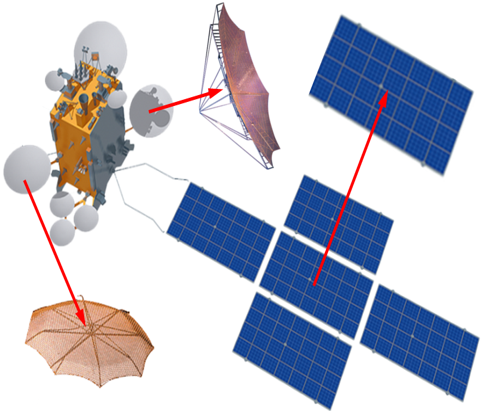
\includegraphics[width = \textwidth]{decomposition}
	\end{subfigure}
	\hfill
	\begin{subfigure}[b]{0.45\textwidth}
	     % Определение стиля
        \tikzstyle{blockWide} = [rectangle, draw = black, fill = blue!15, rounded corners, text width = 20em, text centered, minimum height = 1.5em, drop shadow] 
        \tikzstyle{blockWideC} = [blockWide, fill = red!20]
        \tikzstyle{arrow} = [draw, thick, color = black!90, -latex'] 
        \scriptsize 
        % Задание перменных
        \def\nodeDist{0.4cm}
        % Отрисовка блок-схемы
        \begin{tikzpicture}[scale = 1, transform shape]
            % Задание узлов		
            \node (modalTests) [blockWide] {Модальные испытания \\ составных частей конструкции};
            \node (modelUpdating) [blockWide, below = \nodeDist of modalTests] {Коррекция расчетных моделей \\ составных частей  конструкции \\ по результатам испытаний};
            \node (checkInfluence) [blockWide, below = \nodeDist of modelUpdating] {Освобождение расчетных моделей \\ составных частей конструкции};
            \node (buildRealModel) [blockWide, below = \nodeDist of checkInfluence] {Синтез расчетной модели полной \\ конструкции из её составных частей};
            \node (buildMathModel) [blockWide, below = \nodeDist of buildRealModel] {Определение динамических \\ характеристик полной расчетной модели};
            % Соединение узлов
            \draw [arrow] (modalTests.south) -- (modelUpdating.north);
            \draw [arrow] (modelUpdating.south) -- (checkInfluence.north);
            \draw [arrow] (checkInfluence.south) -- (buildRealModel.north);
            \draw [arrow] (buildRealModel.south) -- (buildMathModel.north);
        \end{tikzpicture}
	\end{subfigure}
    \caption{Схема методики верификации расчетных моделей крупногабаритных трансформируемых конструкций} \label{fig:schemeDecomposition}
\end{figure}

Продемонстрируем работу этого подхода на примере тестового космического аппарата из раздела~\ref{struct:perturbation}. Заметим, что низшие формы собственных колебаний, соответствующие упругим движениям конструкции, происходят с преимущественным деформированием панелей солнечный батарей, размещенных на орбитальном и командно-сервисном модулях. Поэтому, с целью исключения конструктивно подобных движений, упростим модель \figref{fig:spacecraft-full-mesh}, оставив только орбитальный модуль и связанные с ним солнечные батареи. Полученная конечно-элементная модель, обладающая девятнадцатью тысячами степеней свободы, приведена на рисунке~\ref{fig:spacecraft-test-mesh}.
\begin{figure}[!htb]
	\centering
	\includegraphics[width = 1\textwidth]{spacecraft-test-mesh}
	\caption{Упрощенная конечно-элементная модель тестового космического аппарата} \label{fig:spacecraft-test-mesh}
\end{figure}

Ключевым элементом корректности решения задачи синтеза является обеспечение наиболее полного описания жесткостных и массовых характеристик узлов сопряжения составных частей: орбитального модуля и панелей солнечных батарей. При детальном рассмотрении это требование оказывается противоречивым. С одной стороны, при жестком закреплении мест стыковки происходит безвозвратная потеря информации о стыковочных степенях свободы. С другой стороны, при проведении испытаний упруго-вывешенной конструкции как составной части, реализуются формы колебаний без существенного деформирования интерфейсных областей. Для снятия этого противоречия предлагается проводить модальные испытания составных частей с использованием вспомогательных устройств, обладающих известными жесткостными и инерционными характеристиками. В этом случае устройства, будучи прикрепленными к интерфейсам, обеспечивают их качественное описание. В предельном случае, когда жесткостные характеристики вспомогательного объекта равны нулю, это соответствует размещению массы. Причем чем больше масса, тем сильнее оказываются деформации в рассматриваемой области~---~более полно раскрываются жесткостные характеристики. После выполнения коррекции дополнительные устройства исключаются из расчетных моделей.

Кроме того, имея в виду достижение физической согласованности скорректированных моделей, предлагается использовать результаты нескольких экспериментов при различных условиях закрепления одной составной части. Так, в рассматриваемом примере, коррекция орбитального модуля производится по частотам свободных колебаний и частотам колебаний~\figref{fig:test-spacecraft-orbital-mode}, которые реализуется при прикреплении больших масс ($ \approx 30 $ \% от массы конструкции) к узлам стыковки. Расчетные модели панелей солнечных батарей вблизи мест стыковки дополняются невесомыми пластинами, свободные ребра которых закреплены жестко. Это позволяет проводить одновременную коррекцию моделей составных частей с различными граничными условиями.

\def\sfSpacecraft{0.44\textwidth}

\begin{figure}[!htb]
	\centering
	\begin{subfigure}[t]{\sfSpacecraft}
		\centering
		\includegraphics[width = \textwidth]{test-spacecraft-orbital-mode-1}
		\caption{} 
	\end{subfigure}
	\hfill
	\begin{subfigure}[t]{\sfSpacecraft}
		\centering
		\includegraphics[width = \textwidth]{test-spacecraft-orbital-mode-2}
		\caption{} 
	\end{subfigure}	
	\begin{subfigure}[t]{\sfSpacecraft}
		\centering
		\includegraphics[width = \textwidth]{test-spacecraft-orbital-mode-3}
		\caption{} 
	\end{subfigure}	
	\hfill
	\begin{subfigure}[t]{\sfSpacecraft}
		\centering
		\includegraphics[width = \textwidth]{test-spacecraft-orbital-mode-4}
		\caption{} 
	\end{subfigure}	
	\caption{Первые четыре упругие формы колебаний орбитального модуля с прикрепленными к узлам стыковки массами~(а~--~г)} \label{fig:test-spacecraft-orbital-mode} 
\end{figure}

Примем в качестве целевых значений частоты собственных колебаний исходных моделей, сведенные в таблице~\ref{tab:targetTestSpacecraft}. Для имитации погрешностей моделирования изменим модули упругости конструктивных элементов составных частей. Так, жесткость рамы панелей солнечных батарей, орбитального модуля и соединительных элементов была понижена на $ 10 $ \% в то время, как модуль упругости солнечных батарей повышен на $ 5 $ \%.

\begin{longtblr}[
	caption = {Целевые значения для коррекции составных частей космического аппарата}, 
	label = {tab:targetTestSpacecraft}
]{
	colspec = {|X[c, -1]|X[c]|X[c]|X[c]|X[c]|},
	width = \textwidth, 
	hlines
}
	\SetCell[r = 3]{c} № тона & \SetCell[c = 4]{c} Частоты собственных колебаний, Гц &&& \\
	& \SetCell[c = 2]{c} Орбитальный модуль &  & \SetCell[c = 2]{c} Панели солнечных батарей & \\
	& Свободный с прикрепленной массой & Свободный & Закрепленные & Свободные \\ \hline
	1 & \SetCell[r = 6]{c} \textbf{---} & \SetCell[r = 6]{c} \textbf{---} & 1.591 & \SetCell[r = 6]{c} \textbf{---} \\
	2 & & & 5.193 & \\
	3 & & & 6.841 & \\
	4 & & & 10.070 & \\
	5 & & & 22.028 & \\
	6 & & & 26.398 & \\
	7 & 8.221 & 15.721 & 42.179 & 11.810 \\
	8 & 8.477 & 15.721 & 42.613 & 13.770 \\
	9 & 8.660 & 21.300 & 46.050 & 29.339 \\
	10 & 8.863 & 21.303 & 58.393 & 33.784 \\
	11 & 9.095 & 24.132 & 67.767 & 42.796 \\
	12 & 10.598 & 24.498 & 68.897 & 51.135 \\
	13 & 10.600 & 24.498 & 85.064 & 58.768 \\
	14 & 11.178 & 31.483 & 88.711 & 61.625 \\
	15 & 15.730 & 31.483 & 93.117 & 72.682 \\
\end{longtblr}

Проведем коррекцию составных частей космического аппарата по девяти частотам собственных колебаний, используя одновременно данные двух виртуальных экспериментов. После этого выполним ассемблирование скорректированных моделей. Полученные погрешности в частотах синтезированной модели сведены в таблице~\ref{tab:resultUpdatingTestSpacecraft}. Дополнительно к этим результатам отметим, что при коррекции составных частей только по данным одного виртуального эксперимента, максимальная погрешность в частотах синтезированной модели составила $ 6.34 $ \%. Такое значительное расхождение свидетельствует в пользу необходимости учета результатов нескольких испытаний при коррекции.

\begin{longtblr}[
	caption = {Результаты коррекции и ассемблирования составных частей тестовой модели космического аппарата}, 
	label = {tab:resultUpdatingTestSpacecraft}
]{
	colspec = {|X[c, -1]|X[c]|X[c]|X[c]|X[c]|},
	width = \textwidth, 
	hlines
}
	\SetCell[r = 3]{c} № тона & \SetCell[c = 4]{c} Погрешность в частотах собственных колебаний, \% &&& \\
	& \SetCell[r = 2]{c} Без коррекции & \SetCell[c = 3]{c} Коррекция по девяти частотам && \\
	& & Панелей & Модуля & Панелей и модуля \\ \hline
	7 & -4.689 & -2.120 & -2.756 & -0.021 \\
	8 & -4.678 & -2.078 & -2.782 & -0.018 \\
	9 & -5.121 & -4.447 & -0.674 & 0.100  \\
	10 & -5.040 & -4.760 & -0.354 & -0.028 \\
	11 & -5.040 & -4.760 & -0.357 & -0.032 \\
	12 & -5.121 & -4.443 & -0.687 & 0.091 \\
	13 & -4.102 & -0.966 & -3.161 & 0.011 \\
	14 & -4.112 & -0.999 & -3.135 & 0.016 \\
	15 & -3.303 & -0.234 & -3.066 & -0.006 \\
	16 & -3.303 & -0.234 & -3.066 & -0.005 \\
\end{longtblr}

Распределение изменений узловых жесткостей по всем линейным степеням свободы для орбитального модуля и панелей солнечный батарей показано на рисунках~\ref{subfig:test-orbital-distribution}~и~\ref{subfig:test-panel-distribution} соответственно. При этом минимальный критерий модального соответствия, связывающий формы собственных колебаний синтезированной модели до и после коррекции, составил $ 0.9996 $.

Сходимость процедуры коррекции показана на рисунке~\ref{fig:test-spacecraft-convergence}. Она оценивалась посредством частотного критерия $ \lVert \mat{\alpha} \rVert_{\max} $:
\begin{equation}
	\alpha_{i, j} = \abs{1 - \frac{f ^ \ast_{i, j}}{f_{i, j}}}, \ i = 1 \hdots s, \ j = 1 \hdots r, \label{eq:convergenceCriterion}
\end{equation}
где $ s $~---~число корректируемых тонов колебаний, $ r $~---~число испытаний (моделей) для коррекции, $ f $ и $ f ^ \ast $~---~текущие и целевые значения частот. 

\begin{figure}[!htb]
	\centering
	\begin{subfigure}[t]{\sfSpacecraft}
		\centering
		\includegraphics[width = \textwidth]{test-spacecraft-orbital-distribution}
		\caption{Орбитальный модуль} \label{subfig:test-orbital-distribution}
	\end{subfigure}
	\hfill
	\begin{subfigure}[t]{\sfSpacecraft}
		\centering
		\includegraphics[height = \textwidth]{test-spacecraft-panel-distribution}
		\caption{Панели солнечных батарей} \label{subfig:test-panel-distribution} 
	\end{subfigure} 
	\caption{Распределение изменений узловых жесткостей по всем линейным степеням свободы при коррекции моделей составных частей по девяти частотам собственных колебаний} 
\end{figure}

\begin{figure}[!htb]
	\centering
	\hspace{\shiftPlot}
	\begin{tikzpicture}[scale = 1]
		\begin{semilogyaxis}[
			xlabel     = {Номер итерации},
			ylabel     = {$ \lVert \mat{\alpha} \rVert_{\max} $}, 
			width      = 12cm,
			grid       = both,
			legend pos = south west,
			legend cell align = left,
			xmin = 0, xmax = 8
		]
			\addplot table {images/partModelUpdating/test-spacecraft-panels-convergence.txt};
			\addplot table {images/partModelUpdating/test-spacecraft-orbital-convergence.txt};
			\legend{Панели солнечных батарей, Орбитальный модуль}
		\end{semilogyaxis}
	\end{tikzpicture}
	\caption{Сходимость алгоритма коррекции при уточнении моделей панелей солнечных батарей и орбитального модуля} \label{fig:test-spacecraft-convergence}
\end{figure}

Время одновременной коррекции орбитального модуля по двум экспериментам составило $ 27 $ минут, а время коррекции панелей солнечных батарей~---~$ 2 $ минуты.

\section{Программная реализация методик коррекции, освобождения и синтеза}

По результатам проведенных исследований был разработан программный комплекс, реализующий методики коррекции, освобождения и синтеза конечно-элементных моделей. Конфигурирование и управление расчетом осуществляется с помощью последовательностей команд, размещенных в текстовых файлах. С целью обеспечения возможности параметризации исследований реализован загрузчик, позволяющий переключать управляющие файлы расчета. Ход работы программ отображается на экране и сохраняется в виде файлов журналов событий (<<лог-файлах>>). 

Исходными данными для расчета являются конечно-элементные модели, представленные в виде: координат узлов; данных разметки; матриц жесткости, масс и демпфирования. Для учета геометрических особенностей конструкций при решении задач коррекции могут использоваться данные плоскостей симметрии, а также координаты узлов, определяющих конструктивно-подобные элементы и области коррекции. Последнее особенно актуально при наличии информации об элементах конструкций, характеризующихся наибольшей неопределенностью в упругих и диссипативных характеристиках~---~они подлежат первоочередной коррекции. Модуль коррекции допускает множественную загрузку моделей для проведения одновременной коррекции по результатам нескольких экспериментов.

Программная платформа не учитывает особенностей построения расчетных моделей, присущих различным конечно-элементным пакетам~---~является универсальной. Это достигается за счет использования единого бинарного формата, обеспечивающего компактное хранение и оперативную загрузку данных моделей. Для выгрузки моделей из конечно-элементного пакета \name{Ansys} используются макросы на языке \name{APDL}. Конвертация моделей, полученных в конечно-элементном комплексе \name{Femap}, проводится посредством авторской утилиты, размещенной на платформе \name{github}~\cite{lib:author:github:pchConverter}. 

Формирование глобальной модели конструкции происходит путем ассемблирования КЭ-моделей подконструкций после коррекции и освобождения по степеням свободы узлов стыковки. Полученные данные: модифицированные модели, данные о корректирующих элементах, частоты и формы колебаний, используются для визуализации и оценки достоверности результатов коррекции, освобождения и ассемблирования. 

\section{Выводы по главе \thechapter}

На основании исследований, изложенных в данной главе, получены следующие основные результаты:
\begin{enumerate}
	\item Разработана методика коррекции упругих и восстановления диссипативных характеристик, состоящая в дополнении исходных конечно-элементных моделей внутренними и внешними корректирующими элементами. Параметры этих элементов являются неизвестными, разыскиваемыми в ходе решения задачи оптимизации по целевым значениям из результатов экспериментального модального анализа. Начальное приближение для коррекции диссипативных характеристик конечно-элементных моделей формируется на основе гипотезы Е.\,С.~Сорокина.
	\item Показана сходимость и устойчивость алгоритма коррекции к погрешностям в целевых значениях частот собственных колебаний. Критерием оценки сходимости являлась мера искажения форм собственных колебаний по критерию модального соответствия.
	\item Создана методика освобождения расчетных моделей от связей, наложенных для проведения модальных испытаний. Суть подхода заключается в том, что матрицы жесткости и масс дополняются степенями свободы, которые отвечают за перемещения и повороты модели как жесткого целого. Методика протестирована на примере упруго-массовой системы и балочной модели самолёта.
	\item Развита методика синтеза глобальной расчетной модели конструкции по результатам испытаний её составных частей. Разработаны рекомендации по выбору граничных условий при проведении экспериментального модального анализа. На примере тестовой модели космического аппарата показано, что использование результатов нескольких экспериментов с разными граничными условиями для каждой из составных частей, ведет к уточнению частот собственных колебаний синтезированной модели.
\end{enumerate}

Основные результаты, изложенные в данной главе, опубликованы в работах~\cite{lib:author:iss2018:synthesis, lib:author:spacecraft:cms, lib:author:nstuEn:synthesis, lib:author:samsc:freeing, lib:author:nstuEn:updating, lib:author:iss2019:synthesis, lib:author:nti2019:updating, lib:author:nsu:synthesis, lib:author:nti2020:updating, lib:author:patent:freeing, lib:author:pnrpu:updating}. Способ определения частот и форм собственных колебаний свободной конструкции по результатам испытаний этой конструкции с наложенными связями зарегистрирован как патент на изобретение~\appref{struct:patents}.	
	\chapter{Результаты модальных испытаний как исходные данные для коррекции расчетных моделей конструкций}

Целью модальных испытаний летательных аппаратов (ЛА) является определение характеристик собственных тонов колебаний конструкций. Они проводятся на всех этапах создания ЛА. Результаты модальных испытаний составных частей (агрегатов, фрагментов) являются исходными данными для коррекции их расчетных моделей. Скорректированные расчетные модели агрегатов позволяют уточнить расчетную модель всего ЛА и повысить эффективность работ по доводке опытного изделия. 

\section{Методика определения модальных параметров по результатам экспериментального модального анализа}

С целью обеспечения возможности эффективного расчета обобщенных характеристик по результатам модальных испытаний, на языке программирования \name{C\#} была разработана программная реализация \name{GenCalc}, позволяющая посредством графического интерфейса \figref{fig:gencalc-interface} гибко менять параметры расчета и исследовать зависимости получаемых характеристик по каждому из способов одновременно. Более того, для оценки качества выделения тона колебаний в программе заложена возможность построения частотного годографа \figref{fig:gencalc-godograph} и параметра монофазности \figref{fig:gencalc-monophase-parameter} колебательной системы.

Необходимо отметить, что составленная программная реализация обеспечивает прямое взаимодействие с результатами модальных испытаний, которые были получены с использованием комплекса \name{Simcenter Testlab}. Это достигается за счет использования программного интерфейса приложения \name{Simcenter Testlab Automation} (\name{API}).

В рамках предлагаемого подхода, для расчетного диапазона необходимо задать минимальный и максимальный уровень амплитуды, число уровней, а также число точек для интерполяции сигнала отклика на каждом уровне. Кроме того, необходимо выбрать частоту амплитудного и фазового резонанса.

Программный функционал позволяет определять логарифмической декремент колебаний системы по каждому тону, используя четыре подхода:
\begin{enumerate}[topsep = 0pt, noitemsep]
	\item По ширине резонансного пика мнимой составляющей сигнала отклика.
	\item По ширине резонансного пика амплитуды колебаний.
	\item По наклону реальной составляющей сигнала отклика.
	\item Посредством точного решения \eqref{eq:generalModalSolution} системы нелинейных уравнений третьего порядка \eqref{eq:generalModalSystem} относительно обобщенных характеристик:
\end{enumerate}

\begin{figure}[!htb]
	\centerfloat
	\includegraphics[width = 0.85\linewidth]{gencalc-interface}
	\caption{Графический интерфейс программы} \label{fig:gencalc-interface}
\end{figure}

\begin{figure}[!htb]
	\centerfloat
	\includegraphics[width = 0.6\linewidth]{gencalc-monophase-parameter}
	\caption{Параметр монофазности по двум каналам возбуждения при колебаниях изделия по антисимметричному тону} \label{fig:gencalc-monophase-parameter}
\end{figure}

\begin{equation}
	\begin{aligned}
		a ^ 3 \sum_{k = 1} ^ M y_k ^ 4 \omega_k ^ 8 - 3 a ^ 2 c \sum_{k = 1} ^ M y_k ^ 4 \omega_k ^ 6 + a \sum_{k = 1} ^ M \left[ y_k ^ 4 \omega_k ^ 4 \left(3 c ^ 2 + h ^ 2 \right) - Q_k ^ 2 y_k ^ 2 \omega_k ^ 4 \right] + \\
		+ \ c \sum_{k = 1} ^ M Q_k ^ 2 y_k ^ 2 \omega_k ^ 2 - c ^ 3 \sum_{k = 1} ^ M y_k ^ 4 \omega_k ^ 2 - c h ^ 2 \sum_{k = 1} ^ M y_k ^ 4 \omega_k ^ 2 = 0, \\
		a ^ 3 \sum_{k = 1} ^ M y_k ^ 4 \omega_k ^ 8 - 3 a ^ 2 c \sum_{k = 1} ^ M y_k ^ 4 \omega_k ^ 6 + a \sum_{k = 1} ^ M \left[ y_k ^ 4 \omega_k ^ 4 \left(3 c ^ 2 + h ^ 2 \right) - Q_k ^ 2 y_k ^ 2 \omega_k ^ 4 \right] + \\
		+ \ c \sum_{k = 1} ^ M Q_k ^ 2 y_k ^ 2 - c ^ 3 \sum_{k = 1} ^ M y_k ^ 4 - c h ^ 2 \sum_{k = 1} ^ M y_k ^ 4 = 0, \\
		a ^ 2 h \sum_{k = 1} ^ M y_k ^ 4 \omega_k ^ 4 - 2 a c h \sum_{k = 1} ^ M y_k ^ 4 \omega_k ^ 2 - h \sum_{k = 1} ^ M Q_k ^ 2 y_k ^ 2 + c ^ 2 h \sum_{k = 1} ^ M y_k ^ 4 + h ^ 3 \sum_{k = 1} ^ M y_k ^ 4 = 0. 
	\end{aligned}
	\label{eq:generalModalSystem}
\end{equation}

Эту систему уравнений удается решить точно:
\begin{equation}
	\begin{gathered}
		a = b ^ {\sfrac{1}{2}}, \\
		c = -\frac{b d_1 + d_3}{d_2 b ^ {\sfrac{1}{2}}}, \\
		h = \left[ \left( \sum_{k = 1} ^ M Q_k ^ 2 y_k ^ 2 - c ^ 2 \sum_{k = 1} ^ M y_k ^ 4 - a ^ 2 \sum_{k = 1} ^ M y_k ^ 4 \omega_k ^ 4 + 2 a c \sum_{k = 1} ^ M y_k ^ 4 \omega_k ^ 2 \right) / \sum_{k = 1} ^ M y_k ^ 4 \right] ^ {\sfrac{1}{2}}, \\ 
		f_1 = \sum_{i, j = 1} ^ M y_i ^ 4 y_j ^ 4 \omega_j ^ 4 \left( \omega_j ^ 4 - \omega_i ^ 4 \right), \ d_1 = \sum_{i, j = 1} ^ M y_i ^ 4 y_j ^ 4 \omega_i ^ 4 \left( w_i ^ 4 - \omega_j ^ 4 \right), \\
		f_2 = \sum_{i, j = 1} ^ M y_i ^ 4 y_j ^ 4 \omega_j ^ 4 \left( \omega_j ^ 2 - \omega_i ^ 2 \right), \ d_2 = 2 \sum_{i, j = 1} ^ M y_i ^ 4 y_j ^ 4 \omega_i ^ 2 \left( w_j ^ 2 - \omega_i ^ 2 \right), \\
		d_3 = \sum_{i, j = 1} ^ M y_i ^ 2 y_j ^ 2 \omega_j ^ 2 \left( y_i ^ 2 Q_j ^ 2 - y_j ^ 2 Q_i ^ 2 \right), \ f_3 = \sum_{i, j = 1} ^ M y_i ^ 2 y_j ^ 2 \omega_i ^ 4 \left( y_i ^ 2 Q_j ^ 2 - y_j ^ 2 Q_i ^ 2 \right), \\
		b = \frac{f_2 d_3 - f_3 d_2}{f_1 d_2 - f_2 d_1}.
	\end{gathered}
	\label{eq:generalModalSolution}
\end{equation}

\begin{figure}[!htb]
	\centerfloat
	\includegraphics[width = 0.6\linewidth]{gencalc-godograph}
	\caption{Частотный годограф в точке отклика изделия при колебаниях по антисимметричному тону} \label{fig:gencalc-godograph}
\end{figure}

В случае последнего подхода будем дополнительно определять обобщенное демпфирование, обобщенные жесткость и массу, и представлять их в виде графической зависимости от уровня амплитуд.

Для выбранной точки отклика конструкции, которая, как правило, располагается вблизи точки возбуждения, выберем некоторый диапазон значений в окрестности резонансной частоты для которого будет проводиться расчет по каждому из подходов. Заметим, что логарифмический декремент изменяется по мере изменения амплитуды воздействия, поэтому, с целью определения характера этого изменения и его предельных значений, предлагается
строить графические зависимости определяемых характеристик от амплитуды отклика.

Рассмотрим каждый из расчетных способов в отдельности. Для отыскания логарифмического декремента колебаний $ \delta_I $ по ширине резонансного пика мнимой составляющей (№1) воспользуемся следующей формулой:

\begin{equation}
	\delta_I = \pi \Delta \overline{f} \sqrt{\frac{\imag \overline{a}}{1 - \imag \overline{a}}}, \label{eq:decrementWidthImaginaryPeak}
\end{equation}
где $ \imag \overline{a} = \frac{\imag a}{\imag a_{\max}} $~---~относительное значение мнимой составляющей сигнала, $ \Delta \overline{f} = \frac{\Delta f}{f_{\imag}}$, $ \Delta f = f_2 - f_1 $~---~разность характерных частот амплитудной частотной характеристики (АЧХ). Значения $ f_1 $ и $ f_2 $ равны абсциссам где ординаты АЧХ достигают (в долях от максимальной амплитуды) характерное значение уровня.

Логарифмический декремент колебаний $ \delta_{II} $ по ширине резонансного пика амплитуды колебаний (№2) рассчитывается следующим образом:
\begin{equation}
	\delta_{II} = \pi \Delta \overline{f} \frac{\overline{A}}{\sqrt{1 - \overline{A} ^ 2}}, \label{eq:decrementWidthAmplitudePeak}
\end{equation}
где $ \overline{A} = \frac{A}{A_{\max}}$~--~относительная характерная амплитуда уровня, $ A = \sqrt{(\real a) ^ 2 + (\imag a) ^ 2} $.

Расчет  $ \delta_{III} $ по наклону реальной составляющей (№3) производится по следующей формуле:
\begin{equation}
	\delta_{III} = \pi \Delta \overline{f},
	\label{eq:decrementAngleReal}
\end{equation}
где значения $ f_1 $ и $ f_2 $ равны абсциссам тех точек, где ординаты АЧХ достигают экстремальных значений. Для определения этих значений предлагается использовать первую производную интерполированной действительной составляющей.

Для определения обобщенных характеристик конструкции из решения системы нелинейных уравнений \eqref{eq:generalModalSystem} необходимо произвести расчет обобщенной силы $ Q $. Для этого воспользуемся выражением:
\begin{equation}
	Q_i = \frac{\sum\limits_{k\,=\,1} ^ p \vline F_i ^ {(k)} \vline \cdot \imag a_i ^ {(k)}}{\imag a_i ^ {\text{ref}}}, \ i = 1 \hdots n,
\end{equation}
где $ n $~---~число отсчетов сигнала, $ \vline F_i ^ {(k)} \vline $~---~амплитуда воздействия в $ k $-ой точке, $ \imag a_i ^ {(k)} $~---~мнимая составляющая отклика сигнала $ k $-ой точке, $ \imag a_i ^ {\text{ref}} $~---~мнимая составляющая отклика сигнала в опорной точке.

Отметим, что расчеты по каждому из способов \eqref{eq:generalModalSolution}, \eqref{eq:decrementWidthImaginaryPeak}~--~\eqref{eq:decrementAngleReal} являются независимыми, поэтому осуществляются параллельно. Такой подход позволяет существенно ускорить производительность вычислений при высокой дискретизации сигнала отклика по уровню амплитуды.

По результатам вычислений было замечено, что изменение длины интерполяции на каждом расчетном уровне вне зависимости от расчетного подхода слабо влияет на результирующие значения обобщенных характеристик.

Также отметим, что собственная частота колебаний, определенная по обобщенным характеристикам в рамках четвертого способа, претерпевает малые изменения по мере роста относительного значения расчетного уровня \figref{fig:gencalc-natural-frequency}.

\begin{figure}[!htb]
	\centering
	\includegraphics[width = 0.6\linewidth]{gencalc-natural-frequency}
	\caption{Пример определения частоты собственных колебаний конструкции по обобщенным характеристикам} \label{fig:gencalc-natural-frequency}
\end{figure}

\section{Диагностика дефектов конструкций по результатам испытаний}

В конструкциях многих технических изделий имеются зазоры (люфты), которые можно условно разделить на два вида. Одни из них~---~зазоры в соединениях составных частей конструкций~---~вводятся для обеспечения нормального функционирования этих соединений. Величины таких зазоров обычно нормируются. Другой вид~---~люфты, возникающие в процессе эксплуатации. Поскольку нормированные зазоры увеличиваются, как правило, в процессе эксплуатации, то оба этих вида могут привести к повышенной нагруженности и износу деталей, изменению динамических характеристик и ухудшению технического состояния изделий. Поэтому зазоры, конечно же, контролируются. Так как большинство технических изделий подвергается вибрационным испытаниям (прочностным, модальным, испытаниям на виброустойчивость), то представляется целесообразной разработка методики диагностики зазоров в этих испытаниях. 

Техническая вибродиагностика машинного оборудования нашла широкое распространение в машиностроении для контроля механических передач, соединительных муфт и подшипников \cite{lib:defects:Tiwari, lib:defects:Bachschmid, lib:defects:Kostjukov, lib:defects:Balickij, lib:defects:Zhukov}. Эти вращающиеся элементы машин при наличии дисбалансов, люфтов, несоосности и изгибов валов генерируют механические колебания. Колебания, регистрируемые на корпусных деталях машин как вибрации, содержат информацию о динамических процессах, которые происходят в работающей машине. Из этого объема информации необходимо выделить такие данные, на основании которых можно идентифицировать дефекты машин и отслеживать развитие этих дефектов \cite{lib:defects:Zhuge, lib:defects:Lacey, lib:defects:Litak}.

Методы вибродиагностики технических изделий по результатам испытаний разделятся на три группы. К первой из групп относятся методы обнаружения дефектов по изменению параметров собственных тонов колебаний \cite{lib:defects:Kisilev, lib:defects:Postnov, lib:defects:Kosicyn, lib:defects:Perera, lib:defects:Dilena, lib:defects:Xu, lib:defects:Barbieri}. Необходимо отметить, что нередко даже относительно большие повреждения слабо сказываются на изменении основных модальных параметров: частот и форм собственных колебаний. Более того, однозначная идентификация дефекта затруднена тем, что модальные параметры являются интегральными характеристиками, а расположение и величина дефекта~---~дифференциальными \cite{lib:defects:Doebling}.

Методы контроля дефектов по параметрам распространения упругих волн образуют вторую группу \cite{lib:defects:Viktorov, lib:defects:Worlton:ultrasonic, lib:defects:Worlton:experimental, lib:defects:Kessler, lib:defects:Zaitsev}. Но неоднородности конструкции в виде отверстий и вырезов осложняют использование этих методов.

Если в техническом изделии, проектные характеристики которого соответствуют линейной динамической системе, возникают суб- и супергармонические резонансы, искажения фазовых и других видов портретов колебаний, например, фигур Лиссажу, то методы обнаружения дефектов по этим признакам можно отнести к третьей группе \cite{lib:defects:Bovsunovsky, lib:defects:Tsifanskiy, lib:defects:Diana, lib:defects:Berns:align, lib:defects:Berns:backlash, lib:defects:AlKhazali, lib:defects:Berns:gap, lib:defects:Berns:experience, lib:defects:Berns:cracks}.

Как показано в работе \cite{lib:defects:Berns:experience}, для обнаружения и оценки величины зазоров в узлах проводки управления отклоняемыми поверхностями самолетов могут быть использованы нелинейные искажения портретов колебаний, которые определяются в модальных испытаниях.

В данном разделе излагается методика контроля зазоров в технических изделиях по искажениям портретов вынужденных колебаний в процессе любых вибрационных испытаний. Представлен способ поэтапного выявления всех зазоров в объекте испытаний, которые приводят к искажениям портретов колебаний. Это позволяет не только идентифицировать зазоры, но и оценивать их величины. В рамках описываемого подхода разработана и введена в программное обеспечение управления испытаниями подпрограмма анализа портретов колебаний. 

\subsection{Методика исследований}

Методика диагностирования дефектов в конструкциях летательных аппаратов по искажениям портретов колебаний заключается в следующем: на конструкции вблизи подвижных соединений и мест стыковки или крепления агрегатов и оборудования, а также в наиболее нагруженных местах устанавливаются датчики ускорений. Затем с помощью источников гармонических вибраций создаются вынужденные колебания конструкции. Эти колебания фиксируются акселерометрами и представляются в виде портретов: вертикальная развертка пропорциональна сигналу датчика, а горизонтальная~---~первой гармонике сигнала, сдвинутой по фазе на $ \sfrac{\pi}{2} $. Такой портрет колебаний для линейной динамической системы является окружностью. Наличие дефектов сопровождается нелинейными искажениями портретов колебаний из-за соударения элементов конструкции в зазорах, схлопывания трещин, трения в вершинах трещин и подвижных соединениях. Для численной оценки искажений из ряда Фурье для портрета колебаний вычитается первая гармоника, в остатке ряда определяется абсолютный максимум за период колебаний, величина которого $ \Psi $ принимается за параметр искажений. Величина параметра $ \Psi $ нормируется и обозначается как $ \xi $. Строится распределения $ \xi $ по объекту контроля. По расположениям локальных максимумов искажений определяются местоположения дефектов.

В расчетах параметра $ \xi $ используются два вида нормирования искажений $ \Psi $, условно названные глобальным и локальным. При глобальном нормировании величина $ \Psi $ относилась к амплитуде первой гармоники в контрольной точке конструкции. Предлагается принимать в качестве контрольной такую точку, в которой амплитуда колебаний первой гармоники наибольшая. В случае локального нормирования имеем:
\begin{equation}
	\xi_i = \frac{\max \ \vline \Psi_i \ \vline}{(A_1)_i},
\end{equation}
где $ (A_1)_i $~---~амплитуда колебаний первой гармоники, $ i $~---~номер канала измерений.

Глобальное нормирование необходимо для анализа распределения искажений портретов колебаний по всему изделию. Поскольку частоты вибрационного нагружения объектов испытаний находятся обычно в окрестности их собственных частот, то нужно исключить появление ложных локальных максимумов искажений. Это происходит из-за того, что некоторые акселерометры могут быть установлены вблизи узлов форм собственных колебаний конструкции.

Локальное нормирование искажений портретов колебаний используется для определения местоположений дефектов в отдельных агрегатах и узлах сопряжения конструкции. Такое нормирование позволяет сопоставить между собой проявления разных дефектов и отследить динамику изменения каждого из них в процессе испытаний или эксплуатации.

В рамках описанной методики была создана программа для контроля дефектов в процессе вибрационных испытаний, которые проводятся с использованием программного комплекса \name{Simcenter Testlab}. Для оценки состояния поврежденности конструкции проводится расчет и построение параметров искажений портретов колебаний, которые позволяют выявлять такие конструкционные дефекты, как зазоры (люфты), трещины и повышенное трение в подвижных соединениях. Исходными данными для расчета являются временные сигналы по выбранным каналам измерения. 

По команде экспериментатора~\figref{subfig:finder-interface-single} она осуществляет расчет параметров искажений портретов колебаний $ \xi $ параллельно по всем каналам измерений, строит распределения искажений по конструкции и запоминает такие распределения. Это позволяет контролировать проявление дефектов в течение вибропрочностных испытаний, а также эксплуатации конструкции путем сравнения полей параметра искажений~\figref{subfig:finder-interface-compare}, записанных для разных состояний изделий. Кроме того, в программе заложена возможность построения искажений портретов колебаний для отдельных агрегатов и узлов сопряжения конструкции, что необходимо, например, для поэтапного контроля дефектов.

\def\sfDefects{0.49\textwidth}

\begin{figure}[!htb]
	\centering
	\begin{subfigure}[t]{\sfDefects}
		\includegraphics[width = 1\textwidth]{finder-interface-single}
		\caption{Режим одиночного расчета} \label{subfig:finder-interface-single}
	\end{subfigure}
	\hfill
	\begin{subfigure}[t]{\sfDefects}
		\includegraphics[width = 1\textwidth]{finder-interface-compare} 
		\caption{Режим сравнения} \label{subfig:finder-interface-compare}
	\end{subfigure}
    \caption{Графический интерфейс программы} 
\end{figure}

Для сохранения результирующих форм и портретов колебаний в навигаторе рабочего проекта, программа использует интерфейс \name{Testlab Automation}.

\subsection{Применение методики для диагностирования зазоров и люфтов}

Методика обнаружения зазоров по искажениям портретов колебаний была использована для диагностирования самолетов в процессе модальных испытаний, а также космических аппаратов открытого исполнения в технологических вибрационных испытаниях. 

На рисунках~\ref{fig:distortion-airplane}~--~\ref{fig:distortion-conjunction-excluded} приведены примеры распределений искажений портретов колебаний, полученные в модальных испытаниях нескольких самолётов. Здесь и далее на рисунках красной цветовой гамме соответствуют области изделий с наибольшими искажениями, а синей~---~с наименьшими. 

\begin{figure}[!htb]
	\centerfloat
	\begin{subfigure}[t]{\sfDefects}
		\includegraphics[width = 0.75\textwidth]{distortion-airplane-forewing}
		\caption{Переднего горизонтального оперения}
	\end{subfigure}
	\hfill
	\begin{subfigure}[t]{\sfDefects}
		\includegraphics[width = 1\textwidth]{distortion-airplane-stabilizer} 
		\caption{Цельноповоротного стабилизатора}
	\end{subfigure}
    \caption{Зазоры в узлах крепления оперения. Глобальная нормировка искажений} \label{fig:distortion-airplane}
\end{figure}

\begin{figure}[!htb]
	\centerfloat
	\includegraphics[width = 0.5\linewidth]{distortion-high-lift}
	\caption{Зазоры в проводках управления механизацией крыла самолёта. Глобальная нормировка искажений на частоте изгиба крыла} \label{fig:distortion-high-lift}
\end{figure}

На рисунке~\ref{fig:distortion-wiring-gap} представлены искажения портретов колебаний для самолёта с безбустерной системой управления (фюзеляж не показан). Видно, что максимумы искажений находятся на руле высоты и триммере из-за зазоров в проводках управления. Исключение этих искажений из рассмотрения приводит к локализации максимума искажений в соединении ручки управления с проводкой управления, где обнаружен повышенный люфт~\figref{fig:distortion-wiring-backlash}.

\begin{figure}[!htb]
	\centerfloat
	\includegraphics[width = 0.6\linewidth]{distortion-wiring-gap}
	\caption{Зазоры в проводке управления рулем высоты и триммером. Глобальная нормировка искажений портретов колебаний \\ a) датчики на ручке управления, b) искажения на руле высоты и триммере} \label{fig:distortion-wiring-gap}
\end{figure}

\begin{figure}[!htb]
	\centerfloat
	\includegraphics[width = 0.6\linewidth]{distortion-wiring-backlash}
	\caption{Люфт в соединении ручки управления с проводкой. Глобальная нормировка искажений портретов колебаний} \label{fig:distortion-wiring-backlash}
\end{figure}

Из представленных результатов следует, что планеры самолетов являются линейно деформируемыми конструкциями. Нелинейные искажения портретов соответствуют колебаниям отклоняемых поверхностей. Необходимо отметить, что представленные результаты не являются частным случаем. На рисунке~\ref{fig:distortion-compare-mitten} приведены распределения искажений портретов колебаний самолетов на разных резонансных частотах нескольких собственных форм колебаний планера. Видно, что качественно результаты практически не отличаются~---~максимальные искажения портретов колебаний соответствуют отклоняемым поверхностям.

\begin{figure}[!htb]
	\centerfloat
	\begin{subfigure}[t]{\sfDefects}
		\includegraphics[width = 1\textwidth]{distortion-compare-mitten-1}
	\end{subfigure}
	\hfill
	\begin{subfigure}[t]{\sfDefects}
		\includegraphics[width = 1\textwidth]{distortion-compare-mitten-2} 
	\end{subfigure} \\ 
	\begin{subfigure}[t]{\sfDefects}
		\vspace{-0.2cm}
		\includegraphics[width = 1\textwidth]{distortion-compare-mitten-3} 
	\end{subfigure}
    \caption{Распределения искажений портретов колебаний для различных резонансных частот планера} \label{fig:distortion-compare-mitten}
\end{figure}

Зазоры, в том числе предусмотренные конструкторской документацией, имеют место и в узлах соединения агрегатов планера. В приведённом примере~\figref{subfig:distortion-compare-conjunction-1} видно, что максимумы искажений приходятся не только на отклоняемые поверхности, но и на концевые части крыла. Если нормировать величины искажений к амплитуде первой гармоники в каждой точке измерения, получится следующее: максимумы искажений соответствуют отклоняемым поверхностям и корневым частям крыла~\figref{subfig:distortion-compare-conjunction-2}.

\begin{figure}[!htb]
	\centerfloat
	\begin{subfigure}[t]{\sfDefects}
		\includegraphics[width = 1\textwidth]{distortion-compare-conjunction-1} 
		\caption{Глобальная нормировка} \label{subfig:distortion-compare-conjunction-1}
	\end{subfigure}
	\hfill
	\begin{subfigure}[t]{\sfDefects}
		\includegraphics[width = 1\textwidth]{distortion-compare-conjunction-2} 
		\caption{Локальная нормировка} \label{subfig:distortion-compare-conjunction-2}
	\end{subfigure}
    \caption{Распределения искажений портретов колебаний для многоцелевого самолета} \label{fig:distortion-compare-conjunction}
\end{figure}

Поскольку в проводках управления и узлах установки флаперонов и стабилизаторов могут быть зазоры, исключим их из рассмотрения. Полученное распределение искажений портретов колебаний~\figref{fig:distortion-conjunction-excluded} указывает на наличие зазоров в узлах стыковки отъемной части крыла с фюзеляжем. По конструкторской документации самолета было установлено, что нижние узлы навески крыла действительно выполняются с гарантированным зазором, допускающим перемещения в вертикальном направлении.

\begin{figure}[!htb]
	\centerfloat
	\includegraphics[width = 0.5\linewidth]{distortion-conjuction-excluded}
	\caption{Исключение показаний датчиков из распределения искажений портретов колебаний для многоцелевого самолета} \label{fig:distortion-conjunction-excluded}
\end{figure}

Космические аппараты (КА) в ходе создания подвергаются технологическим вибрационным испытаниям. Результаты используются для подтверждения качества спроектированной конструкции КА и обеспечения ее вибрационной прочности, в том числе для обнаружения производственно-технологических дефектов. Поскольку наибольшие вибрационные нагрузки воздействуют на КА во время его выведения на орбиту, то испытаниям подвергаются КА в стартовой конфигурации. На рисунке~\ref{fig:spacecraft-scheme} показана конструктивно-компоновочная схема КА открытого исполнения. Силовым каркасом является углепластиковой цилиндр с закрепленными на нем сотовыми плоскими панелями. Оборудование КА (антенны, солнечные батареи и т.д), а также астроплата с датчиками системы ориентации и стабилизации расположены на панелях. Для проведения испытаний КА устанавливается на адаптер, предназначенный для стыковки КА с ракетой-носителем.

Вибрационная диагностики КА проводится в несколько этапов \cite{lib:defects:Berns:experience}. На первом из этапов выполняется вибрационное нагружение низкой интенсивности с целью проверки соответствия динамических характеристик КА их проектным значениям. На втором этапе происходит нагружение КА нормированным вибрационным воздействием. В ходе нагружения могут возникать и развиваться дефекты, например, нарушаться межблочные связи за счет появления зазоров. Третий этап повторяет программу нагружения первого. На основании изменения параметров вибраций: резонансной частоты и амплитуды колебаний; появлению высокочастотных составляющих в отклике КА и сдвигу частотного спектра определяют местоположения и характер дефектов.

\begin{figure}[!htb]
	\centerfloat
	\includegraphics[width = 0.35\linewidth]{spacecraft-scheme}
	\caption{Конструктивно-компоновочная схема космического аппарата \\ 1~---~адаптер, 2~---~панель, 3~---~астроплата, 4~---~рефлекторы антенн, 5~---~панели солнечной батареи, 6~---~узел крепления солнечной батареи} \label{fig:spacecraft-scheme}
\end{figure}

В вибрационных испытаниях КА открытого исполнения используется как гармоническая, так и широкополосная случайная вибрация при акустическом нагружении.

На рисунках~\ref{fig:distortion-spacecraft} и~\ref{fig:distortion-antenna} представлены результаты обнаружения зазоров по искажениям портретов колебаний применительно к конструкциям двух КА. Необходимо отметить, что в испытаниях нагружение этих КА производилось синусоидальной вибрацией, частота которой изменялась по логарифмическому закону. Поскольку вынужденные колебания КА являлись нестационарным процессом, то в окрестностях резонансных частот объектов испытаний выделялись временные сегменты, для которых в глобальной нормировке вычислялись искажения портретов колебаний. Среди всех распределений выбирались те, которым соответствуют наибольшие значения искажений. 

На рисунке~\ref{fig:distortion-spacecraft} показаны распределения искажений портретов колебаний по поверхности одного из испытываемых КА. Это единственный вариант распределений в диапазоне частот колебаний от $ 20 $ до $ 100 $ Гц, в котором искажения портретов превышали погрешности их построения. А наибольшие искажения возникали вблизи узлов установки солнечных батарей, в которых имеются конструктивные зазоры. 

\begin{figure}[!htb]
	\centerfloat
	\includegraphics[width = 0.5\linewidth]{distortion-spacecraft}
	\caption{Проявление зазоров в узлах установки солнечных батарей} \label{fig:distortion-spacecraft}
\end{figure}

На рисунке~\ref{fig:antenna-scheme} представлена схема установки для вибрационных испытаний антенны другого КА и распределение искажений портретов колебаний рефлектора антенны. Точками на рисунке~\ref{fig:distortion-antenna} отмечены места установки датчиков ускорений на поверхности рефлектора. Стрелкой обозначено местоположение дефекта: разрушение клеевого соединения одной из опор рефлектора с его каркасом, в результате чего возник зазор. Этому месту соответствуют и наибольшие искажения портретов колебаний.

\begin{figure}[H]
	\centerfloat
	\includegraphics[width = 0.6\linewidth]{antenna-scheme}
	\caption{Установка для испытаний антенны \\ 1~---~каркас, 2~---~рефлектор, 3~---~вибростенд} \label{fig:antenna-scheme}
\end{figure}

\begin{figure}[!htb]
	\centerfloat
	\includegraphics[width = 0.45\linewidth]{distortion-antenna}
	\caption{Искажения портретов колебаний рефлектора антенны} \label{fig:distortion-antenna}
\end{figure}

\section{Обработка и представление результатов в процессе испытаний}

Одним из ключевых требований обеспечения непрерывности производственного процесса авиационной техники является сокращение времени между натурными испытаниями и первым вылетом изделия. Для удовлетворения этого условия необходимо осуществлять обработку и представление результатов модального анализа непосредственно в процессе испытаний. Это позволит оперативно составить заключение о полноте экспериментальных данных, необходимых для коррекции расчетной модели объекта испытаний. 

Для решения этой задачи авторами на языке программирования \name{C\#} была разработана программа \name{ResponseAnalyzer} для представления результатов модальных испытаний, проведенных с использованием программного комплекса \name{Simcenter Testlab}. Программная реализация использует интерфейс \name{Testlab Automation} для получения и обработки сигналов с датчиков акселерометров, геометрии и информации о ходе проведения эксперимента.

Посредством графического интерфейса~\figref{fig:analyzer-interface} возможен выбор как отдельных геометрических точек конструкции, так и их комбинаций, для построения амплитудно-частотных характеристик на одном и разных уровнях нагружения, форм колебаний, зависимостей резонансных частот собственных колебаний от амплитуд возбуждения. Данные пользовательского выбора сохраняются в виде бинарных шаблонов, которые могут использоваться для обработки результатов повторных испытаний рассматриваемой конструкции. Формой представления результатов работы программы являются электронные таблицы \name{Excel}. В соответствии с пользовательским форматированием этих таблиц происходит размещение результатов. Так, пользователь может поставить в соответствие графическим объектам типа <<Диаграмма>> различные экспериментальные данные, определив стиль и очередность их отображения: толщину и тип линий, параметры маркеров. С целью обеспечения пользовательского контроля результатов обработки, данные, использованные для построения этих графических объектов, наряду со служебной информацией о работе программы, приводятся в одном из разделов результирующих таблиц.

\begin{figure}[!htb]
	\centerfloat
	\includegraphics[width = 0.8\linewidth]{analyzer-interface}
	\caption{Графический интерфейс программы} \label{fig:analyzer-interface}
\end{figure}

Для осуществления выбора сигналов используется раздел навигации \name{Simcenter Testlab} \figref{fig:analyzer-lms-structure}. При этом пользователю доступна загрузка результатов, соответствующих как одному, так и нескольким экспериментам. Кроме того, в случае, когда необходимо исключить выбросы в экспериментальных данных и/или испытания проведены в широком частотном диапазоне, пользователю доступен выбор значений частот для формирования результирующих таблиц.

Взаимодействие с геометрией исследуемого объекта осуществляется с помощью пользовательского ввода и контекстного меню \figref{fig:analyzer-geometry-selection}, в котором доступно для выбора: модель отображения конструкции (полигональная и сетчатая), модель отображения узлов (маркеры и имена), отображение отдельных конструкционных элементов, модель освещения, а также стандартные виды (изометрические и проективные).

\begin{figure}[!htb]
	\centerfloat
	\includegraphics[width = 0.8\linewidth]{analyzer-geometry-selection}
	\caption{Выбор точек конструкции с помощью графического меню} \label{fig:analyzer-geometry-selection}
\end{figure}

\begin{figure}[H]
	\centerfloat
	\includegraphics[width = 0.7\linewidth]{analyzer-lms-structure}
	\caption{Выбор сигналов для построения графических объектов посредством дерева навигации \name{Simcenter Testlab}} \label{fig:analyzer-lms-structure}
\end{figure}

\section{Операционный модальный анализ}

\subsection{Декомпозиция сигналов виброускорений}

Акселерометры нередко используются для записи колебательного процесса в ходе экспериментального модального анализа. Они обладают высокой чувствительностью и позволяют фиксировать высокочастотные составляющие отклика конструкции. 

Временные зависимости перемещений определяются посредством двойного интегрирования сигналов виброускорений. При этом показания акселерометров подвержены влиянию как постоянных факторов, например, воздействию температуры, так и случайных факторов, изменяющихся со временем. Наличие эти шумовых составляющих обуславливает дрейф показаний (тренд) акселерометров, который кратно возрастает при каждом численном интегрировании данных сигналов~\cite{lib:oma:Thong}. Как правило, этот тренд аппроксимируется полиномиально по методу наименьших квадратов~\cite{lib:oma:Gao}. В этом случае неоднозначный выбор степени аппроксимирующего полинома существенно определяет результат вычислений. Известны подходы исключения тренда на основе фильтрации, использующие различные модификации метода скользящего среднего~\cite{lib:oma:Guo}. В рамках этого подхода неправильный выбор ширины временного окна для фильтрации влечет потерю полезных составляющих сигнала.

Модальные характеристики нередко определяются по откликам конструкции на импульсное воздействие. Полагая характер этих возмущений однократным и затухающим, ускорения могут быть представлены в виде, позволяющим автоматически извлекать частоты и логарифмические декременты. В этом случае не возникает необходимости фильтрации тренда. 

Представим ускорения в каждый момент времени как:
\begin{equation}
	\alpha_i(\mat{p}) = \sum\limits_{k\,=\,1} ^ m A_k e ^ {-\eta_k (t_i - t_0)} \sbrackets{\rho_{1,i}(\mat{p}) + \rho_{2, i}(\mat{p})}, \ i = 1 \hdots n. \label{eq:accelDecomposition}
\end{equation}

Гармонические слагаемые, входящие в это разложение, запишутся:
\begin{equation}
	\begin{gathered}
		\rho_{1, i}(\mat{p}) = \cos \sbrackets{\varphi_k + \omega_k (t_i - t_0)} \rbrackets{\eta_k ^ 2 - \omega_k ^ 2}, \\
		\rho_{2, i}(\mat{p}) = 2 \eta_k \omega_k \sin \sbrackets{\varphi_k + \omega_k (t_i - t_0)},
	\end{gathered}
\end{equation}
где $ m $~---~число гармоник в разложении, $ n $~---~число временных отсчетов, $ \eta_k $~---~относительный коэффициент демпфирования, $ \varphi_k $ и $ \omega_k $~---~фаза и частота колебаний. 

Сведем варьируемые параметры разложения в вектор неизвестных:
\begin{equation}
	\mat{p} = 
	\begin{Bmatrix}
		\varphi_k & A_k & \omega_k & \eta_k
	\end{Bmatrix}, \ k = 1 \hdots m.
\end{equation}

Выразим ошибку представления $ \alpha_i(\mat{p}) $ экспериментальных ускорений $ a_i $:
\begin{equation}
	\mat{f(\mat{p})} = 
	\begin{Bmatrix}
		\alpha_0(\mat{p}) - a_0 & \hdots & \alpha_i(\mat{p}) - a_i & \hdots & \alpha_n(\mat{p}) - a_n
	\end{Bmatrix}.
\end{equation}

Таким образом, получаем задачу условной оптимизации:
\begin{equation}
	\begin{aligned}
		\min_{\mat{p}} \quad & \mat{F}(\mat{p}) = \vert \vert \mat{f} \vert \vert ^ 2, \\
		\textrm{s.t.} \quad & 0 \leq \mat{\phi_i} \leq 2 \pi, \\
		 				    			& \mat{w} > 0. \\
	\end{aligned} \label{eq:problemADA}
\end{equation}

Градиент целевой функции имеет вид:
\begin{equation}
	\nabla \mat{F(\mat{p})} = 2 \trans{\mat{J}(\mat{p})} \mat{f(\mat{p})},
\end{equation}
где $ \mat{J}(p) $~---~матрица Якоби по неизвестным параметрам.

Для решения задачи~\eqref{eq:problemADA} будем использовать метод логарифмических барьеров~(внутренней точки). С целью улучшения сходимости, предлагается использовать каскадный вычислительный алгоритм, который постепенно наращивает число гармоник в разложении~\eqref{eq:accelDecomposition}. На каждом шаге итерационного процесса решаются две подзадачи:
\begin{enumerate}
	\item Минимизация ошибок представления $ \mat{f(\mat{p})} $ одной гармоникой. 
	\item Аппроксимация сигнала виброускорений $ \mat{a} $. В качестве начального приближения для $ m $-ой гармоники используется решение задачи частичной минимизации. 
\end{enumerate}
Вычислительные итерации продолжаются до тех пор, пока не достигнуто целевое число гармоник. 

Заметим, что для использования описанного подхода необходимо знание временных границ импульсных фрагментов. 

\subsection{Тестирование на примере имитационной модели ЛА}

Рассмотрим имитационную модель беспилотного летательного аппарата \name{XQ-58 Valkyrie}~\figref{fig:x58-geometry} \cite{lib:misc:x58}. На основании геометрической модели планера была создана конечно-элементная модель \name{Ansys} \figref{fig:x58-mesh}. При этом жесткостные характеристики элементов планера подбирались таким образом, чтобы приблизить спектр частот собственных колебаний к тому, который наблюдается на летательных аппаратах схожей компоновки.

\begin{figure}[!htb]
	\centerfloat
	\includegraphics[width = 0.75\linewidth]{x58-geometry}
	\caption{Геометрическая модель беспилотного летательного аппарата} \label{fig:x58-geometry}
\end{figure}

На каждом из элементов планера была размещена сеть виртуальных датчиков, связанных между собой треугольными полигонами. Пространственная схема расположения датчиков, общее количество которых составило $ 101 $, приведена на рисунке \ref{fig:x58-sensors}.

Для определения модальных характеристик планера к законцовкам крыла было приложено однократное импульсное воздействие длительностью $ 0.04 $ с. Данные динамических откликов записывались с частотой дискретизации $ 2 $ кГц по каждому пространственному направлению во всех датчиках в течение $ 5 $ с. Временные зависимости ускорений вдоль направления Y, полученные в нескольких точках левой консоли крыла, приведены на рисунке~\ref{fig:x58-signals}. Распределение спектральной плотности мощности, соответствующей этим сигналам, показано на рисунке~\ref{fig:x58-spectrums}.

\begin{figure}[!htb]
	\centerfloat
	\includegraphics[width = 0.75\linewidth]{x58-mesh}
	\caption{КЭ-модель беспилотного летательного аппарата} \label{fig:x58-mesh}
\end{figure}

\begin{figure}[!htb]
	\centerfloat
	\includegraphics[width = 0.75\linewidth]{x58-sensors}
	\caption{Схема размещения датчиков} \label{fig:x58-sensors}
\end{figure}

\begin{figure}[!htb]
	\centerfloat
	\includegraphics[width = 1\linewidth]{x58-signals}
	\caption{Временные сигналы ускорений в нескольких точках левой консоли крыла} \label{fig:x58-signals}
\end{figure}

\begin{figure}[!htb]
	\centerfloat
	\includegraphics[width = 1\linewidth]{x58-spectrums}
	\caption{Спектральная плотность мощности в нескольких точках левой консоли крыла} \label{fig:x58-spectrums}
\end{figure}

Необходимо заметить, что не все методы операционного модального анализа, которые рассматриваются в настоящей работе, достаточно эффективны с численной точки зрения для одновременной обработки всего массива данных откликов. Так, посредством метода \name{ERA} удается обработать лишь один элемент планера одномоментно. Наиболее высокопроизводительным и точным применительно к рассматриваемой задачи оказался метод \name{SSI-COV}. В таблице~\ref{tab:x58-ssi-cov-results} сведены частоты $ f $ и логарифмические декременты колебаний $ \delta $, определенные по конечно-элементной модели и методом \name{SSI-COV}. По этим данным вычислены погрешности определения модальных характеристик, которые приведены в двух последних столбцах. При этом определенные формы колебаний \name{SSI-COV} совпадают с расчетными \name{Ansys}. Сравнение форм колебаний на примере пятого тона собственных колебаний приведено на рисунке~\ref{fig:x58-mode-compare}. 

\begin{longtblr}[
	caption = {Результат определения модальных характеристик методом SSI-COV}, 
	label = {tab:x58-ssi-cov-results}, 
]{
	colspec = {|c|c|c|c|c|c|c|},
	hlines
}
	\SetCell[r=2]{c} Тон & \SetCell[c=2]{c} Ansys && \SetCell[c=2]{c} SSI-COV && \SetCell[c=2]{c} Погрешность, \% & \\
	& $ f $, Гц & $ \delta $ & $ f $, Гц & $ \delta $ & $ \Delta \overline{f} $ & $ \Delta \overline{\delta} $ \\ \hline
	1 & 1.8343 & \SetCell[r=11]{c} 0.0628 & 1.8343 & 0.0628 & -0.0018 & 0.0018 \\ 
	2 & 7.0324 & & 7.0322 & 0.0628 & -0.0035 & 0.0050 \\ 
	3 & 10.2304 & & 10.2300 & 0.0628 & -0.0042 & -0.0141 \\ 
	4 & 21.7268 & & 21.7180 & 0.0628 & -0.0405 & -0.0730 \\ 
	5 & 25.9578 & & 25.9430 & 0.0628 & -0.0571 & -0.1016 \\ 
	6 & 30.8802 & & 30.8560 & 0.0627 & -0.0784 & -0.1732 \\ 
	7 & 35.5900 & & 35.5530 & 0.0627 & -0.1039 & -0.2035 \\ 
	8 & 38.4500 & & 38.4030 & 0.0627 & -0.1223 & -0.2369 \\ 
	9 & 40.3791 & & 40.3250 & 0.0626 & -0.1340 & -0.2942 \\ 
	10 & 40.4966 & & 40.4420 & 0.0627 & -0.1348 & -0.2608 \\ 
	11 & 52.6507 & & 52.5310 & 0.0626 & -0.2274 & -0.4486 \\ 
\end{longtblr}

\begin{figure}[!htb]
	\centering
	\begin{subfigure}{0.49\textwidth}
		\includegraphics[width = 1\textwidth]{x58-ansys-mode-5}
		\caption{\name{Ansys}}
	\end{subfigure}
	\begin{subfigure}{0.49\textwidth}
		\includegraphics[width = 1\textwidth]{x58-ssi-cov-mode-5}
		\caption{\name{SSI-COV}}
	\end{subfigure}
     \caption{Сопоставление расчетных и определенных форм собственных колебаний тона №5} \label{fig:x58-mode-compare}
\end{figure}

Остальные формы колебаний, определенные методом \name{SSI-COV}, приведены на рисунках~\ref{subfig:x58-ssi-cov-mode-1}~--~\ref{subfig:x58-ssi-cov-mode-4}.

\def\sfX58{0.48\textwidth}

\begin{figure}[!htb]
	\centering
	\begin{subfigure}[b]{\sfX58}
		\includegraphics[width = \textwidth]{x58-ssi-cov-mode-1}
		\caption{1.83 Гц (траекторный)} \label{subfig:x58-ssi-cov-mode-1}
	\end{subfigure}
	\hfill
	\begin{subfigure}[b]{\sfX58}
		\includegraphics[width = \textwidth]{x58-ssi-cov-mode-2}
		\caption{7.03 Гц}
	\end{subfigure}
	\begin{subfigure}[b]{\sfX58}
		\includegraphics[width = \textwidth]{x58-ssi-cov-mode-3}
		\caption{10.23 Гц}
	\end{subfigure}	
	\hfill
	\begin{subfigure}[b]{\sfX58}
		\includegraphics[width = \textwidth]{x58-ssi-cov-mode-4}
		\caption{21.71 Гц} \label{subfig:x58-ssi-cov-mode-4}
	\end{subfigure}	
	\caption{Пример форм колебаний имитационной модели по методу \name{SSI-COV} (a~--~г)}
\end{figure}

Для количественной оценки соответствия определенных форм колебаний их расчетным аналогам, воспользуемся критерием модального соответствия. Численная оценка качества выделения форм колебаний методом \name{SSI-COV} для первых двенадцати тонов колебаний приведена на рисунке~\ref{fig:x58-mac}. Из рисунка видно, что определенные формы колебаний практически совпадают с расчетными.

Стабилизационная диаграмма, построенная по методу \name{SSI-COV}, показана на рисунке~\ref{fig:x58-ssi-cov}.

\begin{figure}[H]
	\centerfloat
	\includegraphics[width = 1\linewidth]{x58-ssi-cov}
	\caption{Стабилизационная диаграмма по методу \name{SSI-COV}} \label{fig:x58-ssi-cov}
\end{figure}

\begin{figure}[!htb]
	\centerfloat
	\includegraphics[width = 1\linewidth]{x58-mac}
	\caption{Критерий модального соответствия расчетных форм колебаний их определенным аналогам} \label{fig:x58-mac}
\end{figure}

\subsection{Определение модальных характеристик по результатам акустических испытаний}

Определим модальные характеристики рефлектора \figref{fig:reflector-experiment} по результатам отклика на шумовое акустическое воздействие. Для записи откликов использовались акселерометры~\figref{fig:reflector-sensors}, размещенные на поверхности рефлектора в соответствии со схемой, приведенной на рисунке~\ref{fig:reflector-scheme}.

\begin{figure}[!htb]
	\centerfloat
	\includegraphics[width = 1\linewidth]{reflector-experiment}
	\caption{Рефлектор в сборе с испытательной оснасткой} \label{fig:reflector-experiment}
\end{figure}

\begin{figure}[!htb]
	\centerfloat
	\includegraphics[width = 0.9\linewidth]{reflector-sensors}
	\caption{Датчики ускорений, размещенные на поверхности рефлектора} \label{fig:reflector-sensors}
\end{figure}

\begin{figure}[!htb]
	\centerfloat
	\includegraphics[width = 0.9\linewidth]{reflector-scheme}
	\caption{Схема расстановки акселерометров по рефлектору} \label{fig:reflector-scheme}
\end{figure}

Длительность шумового воздействия составила $ 53 $ секунды при частоте дискретизации сигналов равной $ 12800 $ Гц. Пример временных сигналов акселерометров вдоль направления Y показан на рисунке~\ref{fig:reflector-signals}. Спектральная плотность мощности исследуемых сигналов приведена на рисунке~\ref{fig:reflector-spectrums}. Обработка сигналов осуществлялась последовательно вдоль каждого из пространственных направлений тремя методами операционного модального анализа: \name{SSI-COV}, \name{ERA} и \name{SSI-DD}. При этом сигнал шумового воздействия не использовался. Частоты и логарифмические декременты колебаний, полученные посредством каждого из методов, сведены в таблице~\ref{tab:reflector-results}.

Формы колебаний, определенные методами операционного модального анализа, приведены на рисунках~\ref{subfig:reflector-ssi-cov-mode-2}~--~\ref{subfig:reflector-ssi-cov-mode-16}.

\begin{figure}[!htb]
	\centerfloat
	\includegraphics[width = 0.84\linewidth]{reflector-signals}
	\caption{Временные сигналы акселерометров вдоль направления Y} \label{fig:reflector-signals}
\end{figure}

\begin{figure}[!htb]
	\centerfloat
	\includegraphics[width = 0.84\linewidth]{reflector-spectrums}
	\caption{Спектральная плотность мощности временных сигналов акселерометров вдоль направления Y} \label{fig:reflector-spectrums}
\end{figure}

\begin{longtblr}[
	caption = {Результаты определения частот и логарифмических декрементов колебаний методами операционного модального анализа}, 
	label = {tab:reflector-results}, 
]{
	colspec = {|c|c|c|c||c|c|c|},
	hlines
}
	\SetCell[r = 2]{c} Тон & \SetCell[c = 3]{c} Частота, Гц && & \SetCell[c = 3]{c} Логарифмический декремент && \\
	& SSI-COV & ERA & SSI-DD & SSI-COV & ERA & SSI-DD \\ \hline
	1 & 66.052 & 65.962 & 66.403 & 0.054 & 0.042 & 0.045 \\
	2 & 91.287 & 90.910 & 91.843 & 0.030 & 0.052 & 0.042 \\
	3 & 102.540 & --- & --- & 0.056 & --- & --- \\
	4 & 114.770 & --- & --- & 0.063 & --- & --- \\
	5 & 122.370 & --- & --- & 0.094 & --- & --- \\
	6 & 127.850 & --- & --- & 0.049 & --- & --- \\
	7 & 157.560 & --- & --- & 0.121 & --- & --- \\
	8 & 203.850 & --- & --- & 0.060 & --- & --- \\
	9 & 208.270 & --- & --- & 0.062 & --- & --- \\
	10 & 227.700 & --- & --- & 0.057 & --- & --- \\
	11 & 243.360 & --- & --- & 0.048 & --- & --- \\
	12 & 273.450 & 273.310 & --- & 0.033 & 0.026 & --- \\
	13 & 283.300 & --- & 281.990 & 0.040 & --- & 0.033 \\
	14 & 325.360 & --- & 324.020 & 0.034 & --- & 0.056 \\
\end{longtblr}

На основе таблицы~\ref{tab:reflector-results} можем заключить, что метод \name{SSI-COV} позволяет выделить наибольшее число тонов колебаний. Оценим сходимость модальных характеристик, определяемых этим методом: частот~\tabref{tab:reflector-conv-time-frequency} и логарифмических декрементов колебаний~\tabref{tab:reflector-conv-time-decrement}, варьируя длительность временных сигналов от $ 5 $ до $ 50 $ секунд. 

\def\sfReflector{0.48\textwidth}

\begin{figure}[H]
	\centering
	\begin{subfigure}[b]{\sfReflector}
		\includegraphics[width = \textwidth]{reflector-ssi-cov-mode-2}
		\caption{91.29 Гц} \label{subfig:reflector-ssi-cov-mode-2}
	\end{subfigure}
	\hfill
	\begin{subfigure}[b]{\sfReflector}
		\includegraphics[width = \textwidth]{reflector-ssi-cov-mode-6}
		\caption{127.85 Гц}
	\end{subfigure}
	\begin{subfigure}[b]{\sfReflector}
		\includegraphics[width = \textwidth]{reflector-ssi-cov-mode-13}
		\caption{283.30 Гц}
	\end{subfigure}	
	\hfill
	\begin{subfigure}[b]{\sfReflector}
		\includegraphics[width = \textwidth]{reflector-ssi-cov-mode-16}
		\caption{329.54 Гц} \label{subfig:reflector-ssi-cov-mode-16}
	\end{subfigure}	
	\caption{Пример форм колебаний рефлектора, определенных методом \name{SSI-COV} (a~--~г)}
\end{figure}

\begin{longtblr}[
	caption = {Cходимость частот собственных колебаний в зависимости от длины временного сегмента}, 
	label = {tab:reflector-conv-time-frequency}
]{
	colspec = {|c|c|c|c|c|c|c|},
	hlines
}
	\SetCell[r = 2]{c} Тон & \SetCell[c = 6]{c} Длительность сегмента, c &&&&& \\
	& 5 & 10 & 20 & 30 & 40 & 50 \\ \hline
	1 & 66.096 & 65.993 & 66.102 & 66.04 & 66.042 & 66.052 \\
	2 & 91.335 & 91.193 & 91.174 & 91.259 & --- & 91.287 \\
	3 & --- & --- & --- & 102.87 & 102.64 & 102.54 \\
	4 & 115.25 & --- & 114.79 & 114.97 & 114.21 & 114.77 \\
	5 & 124.26 & 119.06 & 122.3 & 122.09 & 122.24 & 122.37 \\
	6 & --- & --- & 130.13 & --- & 128.34 & 127.85 \\
\end{longtblr}

\begin{longtblr}[
	caption = {Cходимость логарифмического декремента колебаний в зависимости от длины временного сегмента}, 
	label = {tab:reflector-conv-time-decrement}
]{
	colspec = {|c|c|c|c|c|c|c|}, 
	hlines
}
	\SetCell[r = 2]{c} Тон & \SetCell[c = 6]{c} Длительность сегмента, c &&&&& \\
	& 5 & 10 & 20 & 30 & 40 & 50 \\ \hline
	1 & 0.060 & 0.041 & 0.052 & 0.052 & 0.051 & 0.054 \\
	2 & 0.027 & 0.027 & 0.025 & 0.027 & --- & 0.030 \\
	3 & --- & --- & --- & 0.060 & 0.057 & 0.056 \\
	4 & 0.081 & --- & 0.070 & 0.073 & 0.068 & 0.063 \\
	5 & 0.086 & 0.090 & 0.098 & 0.101 & 0.096 & 0.094 \\
	6 & --- & --- & 0.022 & --- & 0.043 & 0.049 \\
\end{longtblr}

Дополнительно оценим влияния частоты дискретизации на устойчивость численных значений модальных характеристик, определяемых методом \name{SSI-COV}. Для этого временные отклики прореживаются с интервалами, которые соответствует диапазону частот дискретизации от $ 12800 $ до $ 2560 $ Гц. Результаты по частотам и логарифмическим декрементам сведены в таблицах~\ref{tab:reflector-conv-sample-frequency}~и~\ref{tab:reflector-conv-sample-decrement} соответственно. 

\begin{longtblr}[
	caption = {Cходимость частот собственных колебаний в зависимости от частоты дискретизации}, 
	label = {tab:reflector-conv-sample-frequency}
]{
	colspec = {|c|c|c|c|c|c|}, 
	hlines
}
	\SetCell[r = 2]{c} Тон & \SetCell[c = 5]{c} Частота дискретизации, Гц &&&& \\
	& 12800 & 6400 & 4267 & 3200 & 2560 \\ \hline
	1 & 66.052 & 65.874 & 65.933 & 65.891 & 65.841 \\
	2 & 91.287 & 91.292 & 91.201 & 91.136 & 91.049 \\
	3 & 102.539 & 102.476 & 102.458 & 102.763 & 103.266 \\
	4 & 114.772 & 114.007 & 114.044 & 114.134 & 114.196 \\
	5 & 122.375 & 123.003 & 123.034 & 123.123 & 123.257 \\
	6 & 127.851 & 129.596 & 129.586 & 129.580 & 129.599 \\
\end{longtblr}

\begin{longtblr}[
	caption = {Cходимость логарифмического декремента колебаний в зависимости от частоты дискретизации}, 
	label = {tab:reflector-conv-sample-decrement}, 
]{
	colspec = {|c|c|c|c|c|c|}, 
	hlines
}
	\SetCell[r = 2]{c} Тон & \SetCell[c = 5]{c} Частота дискретизации, Гц &&&& \\
	& 12800 & 6400 & 4267 & 3200 & 2560 \\ \hline
	1 & 0.054 & 0.034 & 0.030 & 0.032 & 0.029 \\
	2 & 0.030 & 0.025 & 0.031 & 0.035 & 0.037 \\
	3 & 0.056 & 0.062 & 0.068 & 0.064 & 0.055 \\
	4 & 0.063 & 0.053 & 0.052 & 0.052 & 0.053 \\
	5 & 0.094 & 0.061 & 0.057 & 0.056 & 0.050 \\
	6 & 0.049 & 0.020 & 0.021 & 0.022 & 0.022 \\
\end{longtblr}

Можем видеть, что временного сегмента длительностью $ 20 $ секунд достаточно для стабилизации численных значений определяемых модальных характеристик.

В случае изменения частоты дискретизации частота собственных колебаний меняется незначительно, в то время как логарифмический декремент колебаний меняется в разы. 

\subsection{Оценка модальных параметров летательных аппаратов по результатам полетов в неспокойной атмосфере}

\fixme{Коротко о сути подходов: развертка, широкополосное и импульсное возбуждения. Пример применения алгоритма. Оценка доверительных интервалов.}

\section{Выводы по главе \thechapter}
	\chapter{Решение практических задач коррекции расчетных моделей} 

В текущей главе рассматривается применение разработанных методик для решения практических задач коррекции, освобождения и синтеза. Развиваются подходы, позволяющие учесть податливость закрепления в условиях эксперимента. 

\section{Коррекция расчетной модели динамически-подобной модели самолета \mbox{Ту-204}}

Для апробации разработанной методики коррекции на примере реальной конструкции была выбрана динамически-подобная модель (ДПМ) самолета \mbox{Ту-204}, выполненная по отсечно-балочной схеме \figref{fig:tu-204-experiment}. Габаритные размеры: размах крыла $ 3172 $ мм, длина фюзеляжа $ 3462 $ мм (масштаб моделирования~$ 1 \div 10 $). Масса модели с датчиками и кабелями составила $ 50.5 $ кг.

\begin{figure}[!htb]
	\centerfloat
	\includegraphics[width = 0.85\textwidth]{tu-204-experiment}
	\caption{Общий вид ДПМ на упругой подвеске} \label{fig:tu-204-experiment}	
\end{figure}

Упругие характеристики фюзеляжа и крыла смоделированы лонжеронами, расположенными по оси жёсткости каждого агрегата. Топливо, коммерческая нагрузка, оборудование, носовая и основные опоры имитировались жёсткими сосредоточенными грузами. Аэродинамические обводы выполнены в виде лёгких отсеков. Для проведения экспериментального модального анализа ДПМ была вывешена на упругой подвеске малой жесткости.

Исходя из типа схематизации ДПМ, первоначально было принято решение о создании балочной КЭ-модели. Распределение массы конструкции считалось дискретным, а распределение жесткостных характеристик~---~линейным по длине каждой из балок. При моделировании по представленной схеме особую сложность составило описание жесткостных характеристик узлов сочленения агрегатов планера. Так, по результатам расчета на собственные частоты и формы колебаний, было выяснено, что балочная расчетная модель некорректно описывает динамическое поведение реальной ДПМ, в связи с чем было принято решение отказаться от ее дальнейшего использования в пользу твердотельной трехмерной модели.

Создание трехмерной геометрической модели \figref{fig:tu-204-geometry-full} проводилось по натурной ДПМ. Геометрические модели крыльевых отсеков не создавались, так как они, в силу конструктивного исполнения ДПМ, являются точечными массами для упругого крыла~---~не вносят жесткостей и не соприкасаются между собой при малых амплитудах колебаний. В силу последнего обстоятельства отсеки и хвостовое оперение при создании КЭ-модели также моделировались дискретными массами с инерционными характеристиками, определенными по соответствующим геометрическим моделям~\figref{fig:tu-204-geometry-masses}. 

\begin{figure}[!htb]
	\centerfloat
	\includegraphics[width = 0.85\textwidth]{tu-204-geometry-full}
	\caption{Геометрическая модель ДПМ} \label{fig:tu-204-geometry-full}
\end{figure}

\begin{figure}[!htb]
	\centerfloat
	\includegraphics[width = 0.85\textwidth]{tu-204-geometry-masses}
	\caption{Геометрическая модель ДПМ без фюзеляжных отсеков и хвостового оперения} \label{fig:tu-204-geometry-masses}
\end{figure}

Для достоверного определения инерционных характеристик исключенных из модели агрегатов их массы были скорректированы по результатам взвешивания. Аналогичная процедура была проведена для моделирования коммерческой загрузки дискретными массами. Отметим, что было достигнуто удовлетворительное согласование масс лонжерона крыла и фюзеляжа расчетной модели с данными технической документации ДПМ.

По выгруженной из \name{Solidworks} геометрической модели была создана КЭ-модель \name{Ansys}~\figref{fig:tu-204-mesh} с числом степеней свободы~---~$ 751871 $. Стандартные инструменты графической оболочки конечно-элементного модуля \name{Ansys Workbench} предусматривают лишь возможность создания дискретных масс без учета центробежных моментов инерции. Поэтому был разработан скрипт на языке \name{Ansys APDL} для расширения существующего инструментария: моделирование дискретных масс по заданным матрицам инерции. 

Расположение дискретных масс, моделирующих агрегаты планера и коммерческую загрузку, формировались посредством графического интерфейса \name{Ansys Workbench} и установления их именного соответствия с инерционными характеристиками (масса, положение и матрица инерции) в текстовом файле. В ходе расчета разработанным скриптом создаются дополнительные массовые элементы \name{Matrix27}, которые присоединяются жесткими невесомыми балками к узлам, принадлежащим выбранным областям. 

\begin{figure}[H]
	\centerfloat
	\includegraphics[width = 0.85\textwidth]{tu-204-mesh}
	\caption{Конечно-элементная модель ДПМ} \label{fig:tu-204-mesh}
\end{figure}

С целью обеспечения корректности моделирования размер конечного элемента варьировался до тех пор, пока изменение частот собственных колебаний, соответствующее двум последовательным шагам, не оказалось меньшим заданной точности. 

Коррекция КЭ-модели проводилась по шести наборам экспериментально определенных частот собственных колебаний:
\begin{enumerate}
	\item по 7 тону~---~симметричный изгиб крыла I тона~(СИКр1);
	\item с 7 по 8 тон~---~СИКр1, антисимметричный изгиб крыла I тона~(АСИКр1);
	\item с 7 по 9 тон~---~СИКр1, АСИКр1, горизонтальный изгиб фюзеляжа I тона~(ГИФ1);
	\item с 7 по 10 тон~---~СИКр1, АСИКр1, ГИФ1, вертикальный изгиб фюзеляжа I тона (ВИФ1);
	\item с 7 по 10 и 12 тону~---~СИКр1, АСИКр1, ГИФ1, ВИФ1, симметричный изгиб крыла II тона (СИКр2);
	\item с 7 по 10, 12 и 15 тонам~---~СИКр1, АСИКр1, ГИФ1, ВИФ1, СИКр2, вертикальный изгиб фюзеляжа II тона~(ВИФ2).
\end{enumerate}

Итерационный процесс коррекции по предложенному алгоритму считался завершенным при достижении
целевых значений частот с точностью 0.0001 \%. Результаты коррекции сведены в таблице \ref{tab:updatingTu204}.

\begin{longtblr}[
	caption = {Результаты коррекции ДПМ самолета \mbox{Ту-204}}, 
	label = {tab:updatingTu204}
]{
	colspec = {|c|c|c|c|X[c]|X[c]|X[c]|X[c]|X[c]|X[c]|}, 
	hlines
}
   	\SetCell[r = 3]{c} Тон & \SetCell[c = 2]{c} Частоты, Гц && \SetCell[c = 7]{c} Погрешность до и после коррекции, \%  \\
   	& \SetCell[r = 2]{c} Эксперимент & \SetCell[r = 2]{c} {Исходная \\ модель} & \SetCell[r = 2]{c} До & \SetCell[c = 6]{c} После \\ 
   	& & & & 1 & 2 & 3 & 4 & 5 & 6 \\ \hline
	СИКр1 & 3.44 & 3.49 & 1.5 & 0.0 & 0.0 & 0.0 & 0.0 & 0.0 & 0.0 \\
	АСИКр1 & 4.87 & 4.96 & 1.7 & -0.6 & 0.0 & 0.0 & 0.0 & 0.0 & 0.0 \\
	ГИФ1 & 5.44 & 5.73 & 5.3 & 4.7 & 4.7 & 0.0 & 0.0 & 0.0 & 0.0 \\ 
	ВИФ1 & 5.73 & 5.97 & 4.2 & 3.5 & 3.3 & 2.6 & 0.0 & 0.0 & 0.0 \\
	СИКр2 & 9.30 & 9.13 & -1.8 & -4.4 & -3.2 & -3.9 & -4.4 & 0.0 & 0.0 \\
	ВИФ2 & 14.18 & 14.77 & 4.2 & 3.7 & 3.8 & 3.4 & 2.0 & 3.3 & 0.0 \\
\end{longtblr}

Распределения изменений узловых жестокостей по всем линейным степеням свободы КЭ-модели до и после каждой из коррекций
приведены на рисунке~\ref{fig:tu-204-coeffs}.

\def\sfTu204Dist{0.4\textwidth}

\begin{figure}[H]
	\centering
	\begin{subfigure}[b]{\sfTu204Dist}
		\includegraphics[width = \textwidth]{tu-204-coeffs-1}
		\caption{} \label{subfig:tu-204-coeffs-1}
	\end{subfigure}
	\begin{subfigure}[b]{\sfTu204Dist}
		\includegraphics[width = \textwidth]{tu-204-coeffs-2}
		\caption{}
	\end{subfigure}
	\begin{subfigure}[b]{\sfTu204Dist}
		\includegraphics[width = \textwidth]{tu-204-coeffs-3}
		\caption{}
	\end{subfigure}	
	\begin{subfigure}[b]{\sfTu204Dist}
		\includegraphics[width = \textwidth]{tu-204-coeffs-4}
		\caption{}
	\end{subfigure}	
	\begin{subfigure}[b]{\sfTu204Dist}
		\includegraphics[width = \textwidth]{tu-204-coeffs-5}
		\caption{}
	\end{subfigure}
	\begin{subfigure}[b]{\sfTu204Dist}
		\includegraphics[width = \textwidth]{tu-204-coeffs-6}
		\caption{} \label{subfig:tu-204-coeffs-6}
	\end{subfigure}
	\caption{Распределения изменений узловых жесткостей при коррекции по наборам целевых частот от 1 до 6 (а~--~е)} \label{fig:tu-204-coeffs}
\end{figure}

Синяя цветовая гамма на рисунке соответствует областям понижения исходной жесткости (корректирующая КЭ-модель имеет отрицательную жесткость в этих областях), а красная~---~областям повышения исходной жесткости. Черному цвету соответствуют области, жесткость которых в ходе коррекции осталась неизменной.

Заметим, что коррекция по одному тону (набор 1) приводит к снижению жесткости практически во всех областях~\figref{subfig:tu-204-coeffs-1} с измененной жесткостью. Добавление в набор других тонов приводит к появлению областей с положительным изменением жесткости в узлах (рисунки \ref{subfig:tu-204-coeffs-1}~--~\ref{subfig:tu-204-coeffs-6}). При этом для каждого набора распределение корректирующих жесткостей уникально.

Вследствие изменения упругости корректируемой модели происходит изменение частот и форм колебаний. Нормированные к массе формы колебаний до (серым цветом) и после коррекции (зеленым цветом) по шестому набору частот приведены на рисунке \ref{fig:tu-204-modes}. Из рисунка видно, что формы колебаний до и после коррекции хорошо коррелируют между собой, разница между формами колебаний по MAC-критерию до и после коррекции составила: $ 0.02 $, $ 1.12 $, $ 1.74 $, $ 0.87 $, $ 0.18 $ и $ 4.09 $\,\% соответственно.

\def\sfTu204Mode{0.32\textwidth}

\begin{figure}[H]
	\centering
	\begin{subfigure}[b]{\sfTu204Mode}
		\centering
		\includegraphics[width = \textwidth]{tu-204-mode-1}
		\caption{СИКр1} 
	\end{subfigure}
	\begin{subfigure}[b]{\sfTu204Mode}
		\centering
		\includegraphics[width = 0.65\textwidth]{tu-204-mode-2}
		\caption{АСИКр1}
	\end{subfigure}
	\begin{subfigure}[b]{\sfTu204Mode}
		\centering
		\includegraphics[width = \textwidth]{tu-204-mode-3}
		\caption{ГИФ1}
	\end{subfigure}	
	\begin{subfigure}[b]{\sfTu204Mode}
		\centering
		\includegraphics[width = \textwidth]{tu-204-mode-4}
		\caption{ВИФ1}
	\end{subfigure}	
	\begin{subfigure}[b]{\sfTu204Mode}
		\centering
		\includegraphics[width = 0.7\textwidth]{tu-204-mode-5}
		\caption{СИКр2}
	\end{subfigure}
	\begin{subfigure}[b]{\sfTu204Mode}
		\centering
		\includegraphics[width = \textwidth]{tu-204-mode-6}
		\caption{ВИФ2} 
	\end{subfigure}
	\caption{Формы колебаний ДПМ до и после коррекции} \label{fig:tu-204-modes}
\end{figure}

\section{Синтез имитационной модели каркаса зонтичной антенны космического аппарата}

С целью апробации методики синтеза была выбрана имитационная модель каркаса зонтичной антенны~\figref{fig:simsat-assembly}. Каркас выполнен из профилированных стальных труб и плоских стальных накладок. Конструктивно модель состоит из зонтичного каркаса и штанги, элементы скреплены болтами. Габаритные размеры показаны на рисунке~\ref{fig:simsat-dimensions}. Масса каркаса $ 73 $ кг, штанги~---~$ 22 $ кг.

\begin{figure}[!htb]
	\centerfloat
	\includegraphics[width = 0.75\linewidth]{simsat-assembly}
	\caption{Общий вид имитационной модели каркаса зонтичной антенны} \label{fig:simsat-assembly}
\end{figure}

\begin{figure}[H]
	\centerfloat
	\includegraphics[width = 0.65\linewidth]{simsat-dimensions}
	\caption{Габаритные размеры модели каркаса зонтичной антенны} \label{fig:simsat-dimensions}
\end{figure}

\subsection{Модальные испытания}

В соответствии с предлагаемым расчетно-экспериментальным методом, конструкция разделена на две составные части \figref{fig:simsat-parts}: зонтичный каркас и штангу, для каждой из которых проведен экспериментальный модальный анализ.

\begin{figure}[!htb]
	\centering
	\begin{subfigure}[t]{0.48\textwidth}
		\centering
		\includegraphics[width = \textwidth]{simsat-antenna}
		\caption{Зонтичный каркас}
	\end{subfigure}
	\hfill
	\begin{subfigure}[t]{0.48\textwidth}
		\centering
		\includegraphics[width = \textwidth]{simsat-handle}
		\caption{Штанга}
	\end{subfigure}	
	\caption{Составные части модели каркаса зонтичной антенны} \label{fig:simsat-parts}
\end{figure}

Для управления возбуждением и измерением колебаний использовалась многоканальная система \name{LMS SCADAS Lab} \figref{fig:lms-scadas}, включавшая в себя персональный компьютер со специализированным программным обеспечением \name{LMS TestLab}. Система измерений состояла из $ 19 $ блоков восьмиканальных измерительных усилителей стандарта \name{IEPE} ($ 152 $ входных канала). Управление возбуждением колебаний осуществлялось шестиканальным генератором сигналов, позволяющим независимое варьирование амплитудой и фазой сигнала каждого канала. Возбуждение колебаний объекта испытаний осуществлялось электродинамическими силовозбудителями (ЭДСВ) \name{2060E} с усилителями мощности модели \name{2050E09}  производства компании \name{TMS} \figref{fig:simsat-handle-test}. Максимальное номинальное усилие, развиваемое ЭДСВ~---~$ 267 $ Н. Измерение сил проводилось датчиками динамической силы модели \name{208C02} производства компании \name{PCB Piezotronics}. Возбуждающие силы прикладывались к элементам конструкции через стержни с малой изгибной жёсткостью. Виброускорения объекта испытаний измерялись в контрольных точках конструкции акселерометрами стандарта \name{IEPE} модели \name{333B30} производства компании \name{PCB Piezotronics} и модели \name{АР2043-100} производства \name{Глобалтест} \figref{fig:simsat-handle-test}. Акселерометры крепились на поверхность объекта с помощью восковой мастики.

\begin{figure}[!htb]
	\centerfloat
	\includegraphics[width = 0.6\linewidth]{lms-scadas}
	\caption{Система управления испытаниями \name{SCADAS Lab}} \label{fig:lms-scadas}
\end{figure}

\begin{figure}[!htb]
	\centerfloat
	\includegraphics[width = 0.6\linewidth]{simsat-handle-test}
	\caption{Модальные испытания штанги: 1~---~ЭДСВ, 2~---~акселерометр} \label{fig:simsat-handle-test}
\end{figure}

Расчётные исследования скорректированной по результатам испытаний математической модели показали, что узел крепления штанги к силовой колонне имеет недостаточную жёсткость в боковом направлении. Поэтому конструкция кронштейна была изменена \figref{fig:simsat-handle-fixture}. 

\begin{figure}[!htb]
	\centering
	\begin{subfigure}[t]{0.335\textwidth}
		\centering
		\includegraphics[width = \textwidth]{simsat-handle-fixture-init}
		\caption{Исходный}
	\end{subfigure}
	\qquad
	\begin{subfigure}[t]{0.35\textwidth}
		\centering
		\includegraphics[width = \textwidth]{simsat-handle-fixture-improved}
		\caption{Модернизированный}
	\end{subfigure}	
	\caption{Узел крепления имитационной модели к силовой колонне} \label{fig:simsat-handle-fixture}
\end{figure}

Установлено, что закрепление подконструкций на время испытаний в узлах стыковки приводит к потере информации о степенях свободы этих узлов в скорректированной расчётной модели. Поэтому зонтичный каркас был доработан для обеспечения его крепления в центральной части, а не за одну из спиц. На нижней поверхности каркаса установлена гайка с упорами для фиксации его на жёсткой опоре \figref{fig:simsat-antenna-welded}. Собственная частота низшего тона колебаний составила $ 6.095 $~Гц.

\begin{figure}[!htb]
	\centerfloat
	\includegraphics[width = 0.7\linewidth]{simsat-antenna-welded}
	\caption{Узел крепления зонтичного каркаса} \label{fig:simsat-antenna-welded}
\end{figure}

Затем были проведены модальные испытания полностью собранной имитационной модели для проверки результатов коррекции, освобождения и ассемблирования. 

\subsection{Разработка расчетной модели} \label{struct:simsat-model}

Расчетная модель имитационной модели несколько раз уточнялась и претерпевала изменения в связи с отработкой методики ассемблирования и коррекции динамических свойств её составных частей. Прорабатывались такие аспекты, как моделирование узлов стыковки составных частей, моделирование контактного взаимодействия оболочечных элементов при переходе от исходной геометрии к срединным плоскостям. Кроме того, прорабатывались различные варианты крепления штанги к стене из-за невозможности привести динамические параметры модели к параметрам, определенным из эксперимента, что, в итоге, привело к необходимости произвести оценку жесткости крепления штанги к стене. Методика оценки "<жесткости заделки"> описана далее в тексте настоящей работы. Кроме того, проводились исследования с целью определения влияния параметров конечно-элементной сетки на результаты коррекции и последующей виртуальной стыковки моделей составных частей. Каждый из полученных результатов также соотносился с результатами натурных экспериментов. 

После проведенных исследований было принято решение отказаться от контактных элементов и моделировать контактные взаимодействия между срединными плоскостями оболочечными элементами. 

Представленные в настоящей работе результаты по коррекции и стыковке получены по КЭ-модели каркаса зонтичной  антенны с числом степеней свободы~---~$ 252375 $, из которых $ 57852 $~---~штанга, $ 194523 $~---~антенна. На рисунке~\ref{fig:simsat-assembly-mesh} представлена сетка конечных элементов имитационной модели зонтичного каркаса антенны.

\begin{figure}[!htb]
	\centerfloat
	\includegraphics[width = \linewidth]{simsat-assembly-mesh}
	\caption{КЭ-модель имитационной модели в Ansys} \label{fig:simsat-assembly-mesh}
\end{figure}

Идея оценочного расчета <<жесткости заделки>> основана на предположении, что математическая модель конструкции качественно описывает её статическую деформацию, а податливость закрепления вносит поворот конструкции как жесткого целого относительно точки крепления. Для приближенного определения <<жесткости заделки>> рассмотрим следующую расчетную схему \figref{fig:simsat-estimation-scheme}. Видится, что данная схема применима только для протяженных объектов типа штанги.

Приложим силу на конце балки, будем измерять перемещения в двух точках~---~$ A $ и $ B $ \figref{fig:simsat-estimation-scheme}. Представим перемещения точек $ A $ и $ B $~---~$ Y_A, Y_B $ как сумму перемещений от поворота на угол $ \alpha $ как жесткого целого и перемещения $ y_A, y_B $ абсолютно жестко заделанной конструкции под действием приложенной нагрузки. Перемещения $ Y_A, Y_B $ определяются из натурного эксперимента, а перемещения $ y_A, y_B $~---~из виртуального, однако, из-за предполагаемого несоответствия математической модели по количественным показателям, для вывода формулы определения <<жесткости заделки>> будем использовать отношение перемещений, а не их абсолютные значения, предполагая, что математическая модель качественно описывает относительные перемещения конструкции при приложении статической нагрузки.

Положим, что перемещения малы, тогда можно записать следующее соотношение:
\begin{equation}
	\frac{Y_A - \ell_A \sin \alpha}{Y_B - \ell_B \sin \alpha} = \frac{y_A}{y_B}.
	\label{eq:fraction-displacements}
\end{equation}

Из \eqref{eq:fraction-displacements} можно получить выражение для угла:
\begin{equation}
	\alpha = \arcsin \rbrackets{\frac{Y_A - Y_B \frac{y_A}{y_B}}{\ell_A - \ell_B \frac{y_A}{y_B}}}.
	\label{eq:estimated-angle}
\end{equation}

\begin{figure}[!htb]
	\centerfloat
	\begin{tikzpicture}[scale = 1, > = stealth]
		% Задание переменных
		\pgfmathsetmacro{\L}{12} 
		\pgfmathsetmacro{\angle}{20}
		\pgfmathsetmacro{\RPoint}{0.1}
		% Стили
		\tikzstyle{lineStart} = [fill = blue!15]
		\tikzstyle{point} = [draw = black!50, fill = black!20, thick, inner sep = 0pt, minimum size = 2mm]
		\tikzstyle{basedim} = [<->, very thick]
		\tikzstyle{curlydim} = [decorate, very thick]
		\tikzstyle{beamdim} = [curlydim, decoration = {calligraphic brace, mirror, raise = 5pt, amplitude = 6pt}]
		% Недеформированная балка
		\begin{scope}[dashed, thin, color = black, scale = 2]
			\point{s}{0}{0}; \support{3}{s}[-90];
		\end{scope}
		\draw[very thick, black] (0, 0) coordinate (orig) -- (\L, 0) coordinate (endInit);
		% Деформированная балка
		\begin{scope}[scale = 2, blue]
			\point{sr}{0}{0}; \support{3}{sr}[-90-\angle];
		\end{scope}
		\draw[ultra thick, blue] (0, 0) .. controls (3, -0.35) and (6, -1) .. (11.3, -2.5);
		% Повернутая балка
		\draw[thick, black] (0, 0) -- (11.75, -1.3) coordinate (endRot);
		% Точки
		\draw[point] (9, 0) circle (\RPoint) node (B) [above right = 2mm] {$ B $};
		\draw[point] (11, 0) circle (\RPoint) node (A) [above right = 2mm] {$ A $};
		% Размеры
			% A
		\draw[basedim] (10.5, -2.2) -- (10.7, -1.25) node [midway, left = 0.5mm] {$ y_A $};
		\draw[beamdim] (10.5, -2.2) -- (11, 0) node [midway, above right, xshift = 3.5mm, yshift = -2mm] {$ Y_A $};
			% B
		\draw[basedim] (8.6, -1.75) -- (8.8, -1) node [midway, left = 0.5mm, yshift = 0.1mm] {$ y_B $};
		\draw[beamdim] (8.6, -1.75) -- (9, 0) node [midway, above right, xshift = 3.5mm, yshift = -2mm] {$ Y_B $};
			% До точек
		\draw[curlydim, decoration = {calligraphic brace, raise = 3pt, amplitude = 15pt}] (0, 0) -- (9, 0) node [midway, above = 3mm, xshift = 5mm] {$ l_B $};
		\draw[curlydim, decoration = {calligraphic brace, raise = 3pt, amplitude = 45pt}] (0, 0) -- (11, 0) node [midway, above = 12mm, xshift = 6mm, yshift = 0mm] {$ l_A $};
		% Нагрузка
		\draw[line width = 3pt, ->] (\L, 2.5) -- (\L, 0) node [midway, right] { $ P $ };
		\draw[basedim] (0, 2.25) --++ (\L, 0) node [midway, above = 0.5mm] {$ l_P $};
		\draw (0, 0) -- (0, 2.5);
		% Угол
		\draw pic [draw, <-, very thick, angle radius = 6cm] {angle = endRot--orig--endInit};
		\draw (6.3, -0.35) node {$ \alpha $};
		\draw (0, 1) coordinate (startSup) -- (orig) -- (0.75, 2) coordinate (endSup)
        	pic [draw, <-, very thick, angle radius = 1.5cm] {angle = endSup--orig--startSup};
        \draw (0.3, 1.75) node {$ \alpha $};
	\end{tikzpicture}
	\caption{Расчетная схема <<жесткости заделки>>} \label{fig:simsat-estimation-scheme}
\end{figure}

С помощью выражения для угла \eqref{eq:estimated-angle} можно рассчитать <<жесткость заделки>>, зная расстояние до приложенной силы $ \ell_P $, но в зависимости от принятой математической модели упругой заделки целесообразно выражать конкретные параметры. Примем модель <<упругой заделки>> в виде четырехугольной абсолютно жесткой невесомой пластины с четырьмя одинаковыми пружинами \figref{fig:simsat-fixture-scheme}, которая может поворачиваться только в горизонтальном и вертикальном направлениях. Такой шарнир реализуется запрещением всех перемещений центральной точки пластины~--~центра поворота и запрещением перемещений из плоскости всем остальным точкам пластины. Таким образом, пластина может только поворачиваться в двух плоскостях (при условии малости перемещений).

Параметрами, которые подлежат определению для создания модели, являются жесткости пружин $ c $ и размеры пластины $ a $ и $ b $. При этом необходимо проводить два эксперимента для расчета двух углов по горизонтали и вертикали по формуле \eqref{eq:estimated-angle}. Пусть один размер, например $ b $, задается расчетчиком из соображений адекватности исследуемой конструкции. Соответствующая система уравнений имеют вид:
\begin{equation}
	\begin{cases}
		c \sin \alpha_1 a ^ 2 = P_1 \ell_1, \\
		c \sin \alpha_2 b ^ 2 = P_2 \ell_2.
	\end{cases}
\end{equation}

Для такой модели можно получить выражения для размера пластины и жесткости пружин:
\begin{equation}
	a = b \sqrt{\frac{P_1}{P_2} \frac{\ell_1}{\ell_2} \frac{\sin \alpha_2}{\sin \alpha_1}}, \ c = \frac{P_1 \ell_1}{a ^ 2 \sin \alpha_1}. \label{eq:simsat-estimation-final}
\end{equation}

Для определения параметров жесткости крепления штанги к стене проведены дополнительные статические испытания. Нагрузка прикладывалась в концевом сечении штанги вдоль осей $ \mathrm{Y} $ и $ \mathrm{Z} $ соответственно. Регистрация перемещений велась в двух сечениях по длине штанги в соответствии со схемой~\ref{fig:simsat-fixture-scheme}. Результаты экспериментов использованы для определения параметров заделки по формулам~\eqref{eq:simsat-estimation-final}. По рассчитанным данным конечно-элементная модель штанги дополнена моделью <<упругой заделки>>. 

\begin{figure}[H]
	\centerfloat
	\begin{tikzpicture}[scale = 0.95, isometric]
		% Задание переменных
		\pgfmathsetmacro{\width}{8}
		\pgfmathsetmacro{\height}{5}
		\pgfmathsetmacro{\length}{3}
		\pgfmathsetmacro{\hWall}{2}
		\pgfmathsetmacro{\dWall}{0.5}
		\pgfmathsetmacro{\hFixS}{2}
		\pgfmathsetmacro{\hFixE}{1}
		\pgfmathsetmacro{\wFix}{2.5}
		\pgfmathsetmacro{\sD}{2}
		\pgfmathsetmacro{\eD}{0.4}
		\pgfmathsetmacro{\op}{0.95}
		% Стили
		\tikzstyle{plate} = [ultra thick, fill = blue!30, draw = black, opacity = \op]
		\tikzstyle{fixture} = [ultra thick, fill = green!10, draw = black, opacity = \op]
		\tikzstyle{spring} = [thick, color = black, decoration = {aspect = 0.3, segment length = 3mm, amplitude = 3mm, coil}, decorate]
		\tikzstyle{wall} = [pattern = north west lines, pattern color = black]
		% Координаты пластины
		\coordinate (lb) at (-\width/2, 0, 0);
		\coordinate (lt) at (-\width/2, \height, 0);
		\coordinate (rb) at (\width/2, 0, 0);
		\coordinate (rt) at (\width/2, \height, 0);
		% Пружины
		\draw[spring] (rt) --++ (0, 0, -\length) coordinate (rtw) node [midway, above left = 2mm] { $ c $ };
		\draw[wall] (rtw) ++ (0, \hWall/2, 0) --++ (0, -\hWall, 0) --++ (0, 0, -\dWall) --++ (0, \hWall, 0) -- cycle;
		\draw[spring] (rb) --++ (0, 0, -\length) coordinate (rbw) node [midway, above left = 2mm] { $ c $ };
		\draw[wall] (rbw) ++ (0, \hWall/2, 0) --++ (0, -\hWall, 0) --++ (0, 0, -\dWall) --++ (0, \hWall, 0) -- cycle;
		\draw[spring] (lt) --++ (0, 0, -\length) coordinate (ltw) node [midway, above left = 2mm] { $ c $ };
		\draw[wall] (ltw) ++ (0, \hWall/2, 0) --++ (0, -\hWall, 0) --++ (0, 0, -\dWall) --++ (0, \hWall, 0) -- cycle;
		\draw[spring] (lb) --++ (0, 0, -\length) coordinate (lbw) node [midway, above left = 2mm] { $ c $ };
		\draw[wall] (lbw) ++ (0, \hWall/2, 0) --++ (0, -\hWall, 0) --++ (0, 0, -\dWall) --++ (0, \hWall, 0) -- cycle;
		% Пластина
		\draw[plate] (lb) -- (lt) -- (rt) -- (rb) -- cycle;
		% Крепление
		\draw[fixture] (-\width/15, \height/4, 0) --++ (0, 0, \wFix) --++ (0, \hFixE, 0) --++ (0, -\hFixE+\hFixS, -\wFix) -- cycle;
		\draw[fixture] (\width/15, \height/4, 0) --++ (0, 0, \wFix) --++ (0, \hFixE, 0) --++ (0, -\hFixE+\hFixS, -\wFix) -- cycle;
		% Вспомогательные линии для размеров
		\draw (lb) --++ (0, -\sD-\eD, 0);
		\draw (rb) --++ (0, -\sD-\eD, 0);
		\draw (lb) --++ (-\sD-\eD, 0, 0);
		\draw (lt) --++ (-\sD-\eD, 0, 0);
		% Размеры
		\draw[dim<->] (-\width/2, -\sD, 0) --++ (\width, 0, 0) node[midway, below] {$ b $};
		\draw[dim<->] (-\width/2-\sD, 0, 0) --++ (0, \height, 0) node[midway, left] {$ a $};
	\end{tikzpicture}
	\caption{Модель <<упругой заделки>> для штанги} \label{fig:simsat-fixture-scheme}
\end{figure}

В таблице~\ref{tab:simsat-handle-experiment} сведены первые семь частот собственных колебаний, рассчитанных по модели с <<нормальной (идеальной) заделкой>>, с <<упругой заделкой>> и определенные экспериментально. Из таблицы видно, что учет упругости закрепления позволил снизить частоты, но они всё равно остались выше определенных экспериментально, что не противоречит теории.

\begin{longtblr}[
	caption = {Частоты собственных колебаний колебаний штанги}, 
	label = {tab:simsat-handle-experiment}
]{
	colspec = {|c|c|c|c|}, 
	hlines
}
   	\SetCell[r = 2]{c} № тона & \SetCell[c = 3]{c} Частоты, Гц \\
   	& <<Идеальная заделка>> & "<Упругая заделка"> & Эксперимент \\ \hline
	1 & 10.472 & 9.7355 & 9.451 \\
	2 & 13.164 & 12.868 & 12.54 \\ 
	3 & 84.632 & 71.322 & 71.65 \\ 
	4 & 107.51 & 100.45 & 103.4 \\ 
	5 & 171.94 & 155.00 & 171.3 \\ 
	6 & 235.04 & 182.30 & 187.6 \\ 
	7 & 305.87 & 259.05 & 285.2 \\ 
\end{longtblr}

\subsection{Формирование глобальной модели}

Конечно-элементные модели составных частей имитационной модели: штанга и зонтичный каркас, были скорректированы по методу, описанному в разделе~\ref{struct:updating}. В качестве исходных данных для коррекции использовались результаты модальных испытаний. Уточненная модель штанги~\figref{subfig:simsat-handle-model} наряду с распределением изменений узловых жесткостей по всем линейным степеням представлена на рисунке~\ref{subfig:simsat-handle-coefs}.

\begin{figure}[!htb]
	\centering
	\begin{subfigure}[t]{0.46\textwidth}
		\centering
		\includegraphics[width = \textwidth]{simsat-handle-model} 
		\caption{Конечно-элементная сетка} \label{subfig:simsat-handle-model}
	\end{subfigure}
	\hfill
	\begin{subfigure}[t]{0.49\textwidth}
		\centering
		\includegraphics[width = \textwidth]{simsat-handle-coeffs}
		\caption{Распределение корректирующих жесткостей по узлам} \label{subfig:simsat-handle-coefs}
	\end{subfigure}	
	\caption{КЭ-модель штанги с <<упругой заделкой>>} 
\end{figure}

Скорректированная модель зонтичного каркаса освобождена от закрепления по методу, представленному в разделе~\ref{struct:freeing}. Формирование глобальной модели конструкции было проведено путем ассемблирования КЭ-моделей подконструкций по степеням свободы узлов стыковки по принципу формирования глобальной матрицы жесткости в методу конечных элементов.

Также, используя соотношения \eqref{eq:reducedGenParametersUpdating} и \eqref{eq:reducedStructuralMatrices}, была проведена коррекция редуцированных моделей штанги и зонтичного каркаса с последующим ассемблированием. Результаты сведены в таблице~\ref{tab:simsat-combined-results}. 

\begin{longtblr}[
	caption = {Результаты коррекции, освобождения и ассемблирования составных частей имитационной модели}, 
	label = {tab:simsat-combined-results}
]{
	colspec = {|X[c, -1]|X[c]|X[c]|X[c]|X[c]|X[c]|X[c]|}, 
	width = \textwidth, 
	rows = {font = \footnotesize},
	hline{5-12} = {solid}
}
	\hline	
	\SetCell[r = 3]{c} № & \SetCell[c = 6]{c} {Частоты собственных колебаний полной конструкции, Гц \\ (погрешность относительно эксперимента, \%)} \\ \cline{2-7}
	& \SetCell[r = 2]{c} Эксперимент & \SetCell[c = 2]{c} До коррекции && \SetCell[c = 3]{c} После коррекции \\ \cline{3-7}
	&& <<Идеальная заделка>> & <<Упругая заделка>> & Коррекция штанги & Коррекция штанги и антенны & Коррекция редуцированной штанги \\ \hline \hline
	1 & 1.726 & 1.852 (7.27\,\%) & 1.758 (1.84\,\%) & 1.738 (0.70\,\%) & 1.738 (0.70\,\%) & 1.758 (0.66\,\%) \\ 
    2 & 2.248 & 2.383 (6.01\,\%) & 2.335 (3.88\,\%) & 2.241 (0.33\,\%) & 2.239 (0.40\,\%) & 2.335 (2.76\,\%) \\ 
    3 & 5.215 & 5.430 (4.12\,\%) & 5.382 (3.19\,\%) & 5.280 (1.24\,\%) & 5.280 (1.24\,\%) & 5.382 (2.97\,\%) \\ 
    4 & 9.253 & 9.708 (4.92\,\%) & 9.450 (2.13\,\%) & 9.364 (1.18\,\%) & 9.364 (1.18\,\%) & 9.450 (1.78\,\%) \\ 
    5 & 11.98 & 12.44 (3.83\,\%) & 12.25 (2.25\,\%) & 12.32 (2.73\,\%) & 12.22 (1.95\,\%) & 12.25 (1.95\,\%) \\ 
    6 & 26.79 & 27.76 (3.64\,\%) & 27.74 (3.55\,\%) & 27.76 (3.48\,\%) & 27.74 (3.41\,\%) & 27.74 (3.45\,\%) \\ 
    7 & 27.22 & 28.25 (3.78\,\%) & 28.25 (3.78\,\%) & 28.25 (3.64\,\%) & 28.25 (3.64\,\%) & 28.25 (3.64\,\%) 
\end{longtblr}

Из таблицы~\ref{tab:simsat-combined-results} видно, что коррекция моделей составных частей приводит к удовлетворительному совпадению частот ассемблированной модели с соответствующими экспериментальными частотами. Важно отметить, что при коррекции моделей составных частей целевые значения частот были достигнуты с высокой точностью. Кроме того, при коррекции и создании матрицы демпфирования по результатам эксперимента методом \eqref{eq:finalObjFunUpdating} и по формулам \eqref{eq:reducedStructuralMatrices}, \eqref{eq:reducedDampingMatrix} амплитудно-частотные характеристики в окрестности резонансных частот практически совпадают.

На рисунке~\ref{subfig:simsat-mac-absolute} показаны изменения MAC-критерия до и после коррекции четырех низших частот, а на рисунке~\ref{subfig:simsat-mac-relative}~---~значения критерия модального соответствия между исходной и скорректированной моделью. Из рисунков видно, что в ходе коррекции происходит изменение форм собственных колебаний. Наиболее значительно изменилась вторая форма собственных колебаний, но величина этих изменений не превышает $ 0.14 $\,\% в метрике MAC-критерия.

\begin{figure}[H]
	\centering
	\begin{subfigure}[t]{0.49\textwidth}
		\centering
		\includegraphics[width = \textwidth]{simsat-MAC-absolute}
		\caption{Изменение MAC-критерия по абсолютному значению} \label{subfig:simsat-mac-absolute}
	\end{subfigure}
	\hfill
	\begin{subfigure}[t]{0.47\textwidth}
		\centering
		\includegraphics[width = \textwidth]{simsat-MAC-relative}
		\caption{MAC-критерий между исходной и скорректированной моделью} \label{subfig:simsat-mac-relative}
	\end{subfigure}	
	\caption{Оценка связи между формами собственных колебаний до и после коррекции} 
\end{figure}

В таблице~\ref{tab:simsat-full-results} представлены погрешности в определении частот собственных колебаний полноразмерной конструкции после коррекции, освобождения и синтеза моделей составных частей. 

\begin{longtblr}[
	caption = {Результаты полноразмерной коррекции, освобождения и ассемблирования при различном числе корректируемых тонов колебаний}, 
	label = {tab:simsat-full-results}
]{
	colspec = {|X[c, 1.4]|X[c]|X[c]|X[c]|X[c]|X[c]|X[c]|X[c]|X[c]|X[c]|}, 
	width = \textwidth,
	hlines
}
	{Номера \\ тонов} & \SetCell[c = 9]{c} {Погрешности частот скорректированной ассемблированной \\ модели по сравнению с частотами из эксперимента, \%} \\
	Штанги & 1 & 1,\,2 & 1\,--\,3 & 1\,--\,4 & 1\,--\,3 & 1\,--\,3 & 1\,--\,3 & 1\,--\,3 & 1\,--\,4 \\
	Антенны & \SetCell[c = 4]{c} --- &&& & 1 & 1,\,2 & 1,\,15 & 1,\,2,\,15 & 1,\,15 \\ \hline
	1 & -0.90 & -0.90 & 0.70 & 0.70 & 0.70 & 0.70 & 0.70 & 0.70 & 0.70 \\
	2 & 1.16 & 1.47 & 1.47 & -0.33 & 1.41 & 1.43 & 1.39 & 1.40 & -0.40 \\
	3 & 1.50 & 1.50 & 1.24 & 1.24 & 1.23 & 1.21 & 1.23 & 1.21 & 1.24 \\
	4 & 1.40 & 1.40 & 1.18 & 1.18 & 1.18 & 1.17 & 1.18 & 1.17 & 1.18 \\
	5 & 1.44 & 1.49 & 1.49 & 2.73 & 0.91 & 1.16 & 0.71 & 0.78 & 1.95 \\ 
	6 & 3.29 & 3.29 & 3.29 & 3.48 & 3.22 & 3.22 & 3.21 & 3.21 & 3.41 \\ 
	7 & 3.64 & 3.64 & 3.64 & 3.64 & 3.64 & 3.64 & 3.64 & 3.64 & 3.64 \\ 
\end{longtblr}

Можно видеть, что наибольшее влияние на частоты ассемблированной модели оказывает коррекция штанги, в то время как коррекция зонтичного каркаса приводит лишь к небольшому снижению результирующих погрешностей.

\section{Коррекция расчетной модели отъемной части крыла изделия \mbox{С-70}}

В настоящем разделе рассматривается применение метода коррекции к композитной отъемной части крыла (ОЧК) изделия \mbox{С-70}. 

\subsection{Экспериментальный модальный анализ}

Для проведения экспериментального модального анализа консоль крыла была вывешена вертикально на авиационных амортизационных шнурах посредством траверсы \figref{fig:wing-experiment}. Шнуры продевались через установленные в проушины узлов крепления технологические такелажные приспособления. Испытания выполнялись в соответствии методическими рекомендациями \cite{lib:aprobation:Moskalik}. 

\begin{figure}[H]
	\centerfloat
	\includegraphics[width = 0.7\linewidth]{wing-experiment}
	\caption{Общий вид ОЧК изделия \mbox{С-70} на упругой подвеске} \label{fig:wing-experiment}
\end{figure}

\subsection{Построение конечно-элементной модели}

В соответствии с исходными данными, переданными специалистами конструкторского бюро, конструктивно-силовой набор крыла представлялся невесомыми балочными и оболочечными элементами. Последние имеют характеристики обшивки и работают только на растяжение-сжатие, в то время как балочные элементы, лежащие в плоскости симметрии крыла, работают только на изгиб. При этом инерционные характеристик крыла воспроизводятся дискретными массами, имеющими эксцентриситет.

Для формирования геометрической модели использовались таблицы с координатами вершин поверхностей и концевых точек балок. Толщины элементов обшивки задавались дискретно по вершинам, образующим граничные поверхности. Распределение изгибных жесткостей внутри каждой балки описывалось полиномом третьей степени, заданным в равноотстоящих узлах. 

По результатам построения геометрической модели были замечено, что между некоторыми панельными элементами имеются существенные зазоры по высоте~---~нарушена непрерывность геометрического контура. Для обеспечения совместности перемещений элементов составлялись пары контактирующих ребер, которые примыкают друг к другу плоскости симметрии крыла. Кроме того, балочный каркас был спроецирован на обшивку для формирования линий контактного взаимодействия \figref{wing-intersection-isometric}. Массы размещались на ближайших точках балочного каркаса. При этом компоненты тензора инерции пересчитывались пропорционально относительному удалению массы от точки размещения. 

\begin{figure}[!htb]
	\centerfloat
	\includegraphics[width = \linewidth]{wing-intersection-isometric}
	\caption{Проецирование балочного каркаса и масс на элементы силового набора ОЧК} \label{wing-intersection-isometric}
\end{figure}

Посредством системы макросов \name{Ansys Mechanical APDL} была создана программа, позволяющая автоматически формировать конечно-элементную модель при изменении исходных данных. Геометрические модели балочного каркаса и обшивки приведены на рисунках~\ref{fig:wing-geometry-beams} и \ref{fig:wing-geometry-panels} соответственно. Число степеней свободы в модели составило $ 19710 $. Для сшивки панелей как между собой, так и с балочным каркасом, использовались абсолютно жесткие балки. Результирующая конечно-элементная модель приведена на рисунке~\ref{fig:wing-mesh}. Упругие формы собственных колебаний срединной поверхности модели приведены на рисунке~\ref{fig:wing-initial-mode}. Здесь и далее нумерация тонов колебаний начинается с первого тона упругих колебаний. 

\begin{figure}[!htb]
	\centerfloat
	\includegraphics[width = 0.85\linewidth]{wing-geometry-beams}
	\caption{Геометрическая модель балочного каркаса}\label{fig:wing-geometry-beams}
\end{figure}

\begin{figure}[!htb]
	\centerfloat
	\includegraphics[width = 0.85\linewidth]{wing-geometry-panels}
	\caption{Геометрическая модель обшивки}\label{fig:wing-geometry-panels}
\end{figure}

\begin{figure}[H]
	\centerfloat
	\includegraphics[width = 0.85\linewidth]{wing-mesh}
	\caption{Конечно-элементная модель ОЧК} \label{fig:wing-mesh}
\end{figure}

\def\sfWing{0.48\textwidth}

\begin{figure}[!htb]
	\centering
	\begin{subfigure}[t]{\sfWing}
		\centering
		\includegraphics[width = \textwidth]{wing-initial-mode-1}
	\end{subfigure}
	\hfill
	\begin{subfigure}[t]{\sfWing}
		\centering
		\includegraphics[width = \textwidth]{wing-initial-mode-2}
	\end{subfigure}	
	\begin{subfigure}[t]{\sfWing}
		\centering
		\includegraphics[width = \textwidth]{wing-initial-mode-3}
	\end{subfigure}	
	\hfill
	\begin{subfigure}[t]{\sfWing}
		\centering
		\includegraphics[width = \textwidth]{wing-initial-mode-4}
	\end{subfigure}	
	\caption{Пример упругих форм колебаний исходной КЭ-модели ОЧК} \label{fig:wing-initial-mode}
\end{figure}

\subsection{Коррекция конечно-элементной модели}

Коррекция КЭ-модели проводилась по пяти наборам экспериментально определенных частот. Каждый последующий набор дополнял предыдущий одним тоном колебаний. Так, cначала была проведена коррекция только по изгибу ОЧК I тона, а затем еще и по изгибу ОЧК II тона. В конечном итоге была осуществлена одновременная коррекция 5 тонов колебаний \tabref{tab:wing-results}. 

\begin{longtblr}[
	caption = {Результаты коррекции ОЧК}, 
	label = {tab:wing-results}
]{
	colspec = {|c|c|c|X[c]|X[c]|X[c]|X[c]|X[c]|X[c]|}, 
	width = \textwidth, 
	hlines
}
	\SetCell[r = 3]{c} Тон & \SetCell[c = 2]{c} Приведенная частота && \SetCell[c = 6]{c} Погрешность до и после коррекции, \% \\
	& \SetCell[r = 2]{c} Эксперимент & \SetCell[r = 2]{c} {Исходная \\ модель} & \SetCell[r = 2]{c} До & \SetCell[c = 5]{c}После \\
	& & & & 1 & 2 & 3 & 4 & 5 \\ \hline
	1 & 1.00 & 1.51 & 50.7 & 0.0 & 0.0 & 0.0 & 0.0 & 0.0 \\ 
	2 & 2.28 & 3.18 & 39.5 & -7.4 & 0.0 & 0.0 & 0.0 & 0.0 \\ 
	3 & 3.37 & 4.13 & 22.6 & -18.6 & -13.8 & 0.0 & 0.0 & 0.0 \\ 
	4 & 3.95 & 4.82 & 21.8 & -19.1 & -17.8 & -8.2 & 0.0 & 0.0 \\ 
	5 & 4.87 & 6.15 & 26.2 & -16.2 & -21.8 & -2.6 & -4.4 & 0.0 \\ 
\end{longtblr}

Распределения изменений узловых жестокостей по всем линейным степеням свободы КЭ-модели до и после коррекции по первому тону и пяти тонам колебаний приведены на рисунках~\ref{subfig:wing-coeffs-1} и \ref{subfig:wing-coeffs-5} соответственно. Необходимо отметить, что изменения узловых жесткостей при коррекции по пяти тонам посчитаны относительно жесткостей, полученных в результате коррекции по первому тону. Синяя цветовая гамма на рисунках соответствует областям понижения исходной жесткости, а красная~---~областям повышения исходной жесткости. Черному цвету соответствуют области, жесткость которых в ходе коррекции осталась неизменной. 

\begin{figure}[!htb]
	\centering
	\begin{subfigure}[t]{\sfWing}
		\centering
		\includegraphics[width = \textwidth]{wing-coeffs-1}
		\caption{По одному тону} \label{subfig:wing-coeffs-1} 
	\end{subfigure}
	\hfill
	\begin{subfigure}[t]{\sfWing}
		\centering
		\includegraphics[width = \textwidth]{wing-coeffs-5}
		\caption{По пяти тонам} \label{subfig:wing-coeffs-5}
	\end{subfigure}	
	\caption{Распределения изменений узловых жестокостей по всем линейным степеням свободы КЭ-модели до и после коррекции}
\end{figure}

Вследствие изменения упругости корректируемой модели происходит изменение частот и форм колебаний. Нормированные к массе формы колебаний срединной поверхности модели до (черным цветом) и после коррекции (красным цветом) по пяти частотам собственных колебаний приведены на рисунках~\ref{subfig:wing-compare-mode-1}~--~\ref{subfig:wing-compare-mode-5}.

\begin{figure}[!htb]
	\centering
	\begin{subfigure}[t]{\sfWing}
		\centering
		\includegraphics[width = \textwidth]{wing-compare-mode-1}
		\caption{} \label{subfig:wing-compare-mode-1} 
	\end{subfigure}
	\hfill
	\begin{subfigure}[t]{\sfWing}
		\centering
		\includegraphics[width = \textwidth]{wing-compare-mode-2}
		\caption{} 
	\end{subfigure}	
	\begin{subfigure}[t]{\sfWing}
		\centering
		\includegraphics[width = \textwidth]{wing-compare-mode-3}
		\caption{} 
	\end{subfigure}	
	\hfill
	\begin{subfigure}[t]{\sfWing}
		\centering
		\includegraphics[width = \textwidth]{wing-compare-mode-4}
		\caption{} 
	\end{subfigure}	
	\begin{subfigure}[t]{\sfWing}
		\centering
		\includegraphics[width = \textwidth]{wing-compare-mode-5}
		\caption{} \label{subfig:wing-compare-mode-5} 
	\end{subfigure}	
	\caption{Сопоставление первых пяти упругих форм колебаний ОЧК до и после коррекции~(а~--~д)}
\end{figure}

Таблица соответствия форм колебаний до и после коррекции по критерию модального соответствия приведена на рисунке~\ref{fig:wing-mac}. Из рисунка видно, что формы колебаний до и после коррекции удовлетворительно коррелируют между собой.

\begin{figure}[H]
	\centerfloat
	\includegraphics[width = 0.7\linewidth]{wing-mac}
	\caption{Таблица соответствия форм колебаний до и после коррекции} \label{fig:wing-mac}
\end{figure}

\section{Коррекция расчетной модели гирдера для модульных секций накопителя ЦКП <<СКИФ>>}

Центр коллективного пользования <<Сибирский кольцевой источник фотонов>> (ЦКП~<<СКИФ>>) можно условно представить в виде инжекционной части, состоящей из бустерного синхротрона и линейного ускорителя, и накопительного кольца. В первой части происходит создание электронного пучка, обладающего требуемой энергией, который затем преобразуется и накапливается в виде синхротронного излучения в накопительной части. Ключевым требованием к последней является обеспечение максимальной продолжительности жизни пучка и сохранение его интенсивности. Среди прочего, это достигается за счет прецизионного выставления многочисленного электрофизического оборудования на специальных подставках, именуемых гирдерами. К посадочным поверхностям последних предъявляются высокие требования по точности размещения и регулирования. Более того, во избежание возникновения резонансов, приводящих к потере качества пучка, собственные частоты гирдера должны быть отстроены от парциальных частот оборудования и сейсмических колебаний. Решение этой задачи реализуется в три этапа: проектирование, производство и экспериментальная отработка гирдера. Для обоснования и проработки конструкторских решений на первом этапе предлагается использовать метод конечно-элементного моделирования.

В соответствии с конструкторской документаций была построена геометрическая модель гирдера накопительного кольца~\figref{fig:girder-geometry} длиной $ 3800 $ мм (\name{G3800}). Масса гирдера составила $ 2166 $ кг. 

\begin{figure}[H]
	\centering
	\includegraphics[width = 0.6\linewidth]{girder-geometry}
	\caption{Геометрическая модель гирдера} \label{fig:girder-geometry}
\end{figure}

Конструктивное исполнение регулируемых опор гирдера раскрыто на рисунках~\ref{fig:girder-supports} и \ref{fig:girder-support-section}. Особо отметим, что низшие частоты собственных колебаний гирдера в значительной степени обусловлены динамической жесткостью опор.

\begin{figure}[!htb]
	\centering
	\includegraphics[width = 0.7\linewidth]{girder-supports}
	\caption{Регулируемые опоры гирдера} \label{fig:girder-supports}
\end{figure}

\begin{figure}[!htb]
	\centering
	\includegraphics[width = 0.4\linewidth]{girder-support-section}
	\caption{Сечение регулируемой опоры гирдера} \label{fig:girder-support-section}
\end{figure}

Для определения совместного отклика модульной секции магниты размещались на поверхности гирдера согласно рабочей документации института ядерной физики имени Г\,.\,И.~Будкера~СО~РАН \figref{fig:girder-full-system}.

\begin{figure}[!htb]
	\centering
	\includegraphics[width = 0.7\linewidth]{girder-full-system}
	\caption{Совместная геометрическая модель гирдера и магнитов} \label{fig:girder-full-system}
\end{figure}

Необходимо заметить, что крепежные элементы, составные части системы охлаждения совместной системы гирдера и магнитов не оказывают существенного влияния на определяемые статические и динамические характеристики, поэтому геометрическая модель рассматриваемой системы была упрощена. Общие упрощения, использованные при построении конечно-элементных моделей магнитов:
\begin{itemize}
	\item крепежные элементы, не относящиеся к опорам, исключены и заменены контактными элементами;
	\item отверстия, соответствующие отброшенным крепежным элементам, заполнены материалом;
	\item распределение материала по каждому из магнитов считалось изотропным;
	\item плотность материала каждого магнита подбиралась так, чтобы его масса соответствовала массе позиции на чертеже рабочей документации.
\end{itemize} 

Таким образом, была получена упрощенная геометрическая модель системы, на основе которой строилась конечно-элементная модель. Она использовалась для получения первичных оценок напряженно-деформированного состояния под воздействием весовых нагрузок и частот собственных колебаний. 

По результатам расчётов доработано расположение и конструктивное исполнение регулируемых опор. Изменены геометрические параметры фундаментных опор и балок. Конструкция дополнена плитой с целью повышения жесткости гирдера в поперечном направлении. На основании выработанных конструкторских решений гирдер был произведен и испытан средствами экспериментального модального анализа~\figref{fig:girder-experiment}.

\begin{figure}[H]
	\centering
	\includegraphics[width = 0.75\linewidth]{girder-experiment}
	\caption{Модальные испытания гирдера без магнитов} \label{fig:girder-experiment}
\end{figure}

По результатам экспериментальных исследований было установлено, что формы собственных колебаний, соответствующие низшим тонам, происходят при совместном перемещении гирдера и блока фундамента, на который опираются регулируемые опоры~\figref{fig:girder-spring-mode}.

\begin{figure}[!htb]
	\centering
	\includegraphics[width = 0.6\linewidth]{girder-spring-mode}
	\caption{Пример формы колебаний гирдера на упругом основании} \label{fig:girder-spring-mode}
\end{figure} 

Такое упругое поведение фундамента существенно отличается от модели жесткого закрепления, использованной в предварительных расчетах. Было принято решение построить модель упругого основания~\figref{fig:girder-mesh}, используя пружины, жесткости которых определялись автоматически по результатам решения задачи коррекции для первых пяти частот собственных колебаний, отвечающих этим движениям. Целевые значения частот достигнуты со степенью точности $ 2 \cdot 10 ^ {-8} $ по критерию~\eqref{eq:convergenceCriterion}.

\begin{figure}[H]
	\centering
	\includegraphics[width = 0.55\linewidth]{girder-mesh}
	\caption{Конечно-элементная модель гирдера на упругом основании} \label{fig:girder-mesh}
\end{figure}

Полученная модель гирдера на фундаменте использовалась для осуществления одновременной коррекции по шести частотам упругих тонов собственных колебаний~\figref{fig:girder-elastic-mode}. Коррекция КЭ-модели производилась без удержания частот собственных колебаний, соответствующих движениям на упругом основании. Это объясняется отсутствием  экспериментальных данных о характере зависимости частот от уровня приложенных нагрузок. Целевые значения коррекции были достигнуты с высокой степенью точности~\tabref{tab:girder-results}.

\begin{figure}[!htb]
	\centering
	\includegraphics[width = 0.6\linewidth]{girder-elastic-mode}
	\caption{Пример упругой формы колебаний гирдера} \label{fig:girder-elastic-mode}
\end{figure}

\begin{longtblr}[
	caption = {Результаты коррекции гирдера}, 
	label = {tab:girder-results}
]{
	colspec = {|X[c, -1]|X[c]|X[c]|X[c]|X[c]|}, 
	width = \textwidth, 
	hlines
}
	\SetCell[r = 2]{c} Тон & \SetCell[c = 2]{c} Частота, Гц && \SetCell[c = 2]{c} Погрешность, \% \\
	& Эксперимент & Исходная модель & До коррекции & После коррекции \\ \hline
	6 & 119.51 & 135.08 & 13.03 & \SetCell[r = 6]{c} \textbf{0.00} \\
	7 & 140.97 & 146.46 & 3.89 &  \\
	8 & 148.13 & 160.07 & 8.06 &  \\
	9 & 189.65 & 210.48 & 10.98 & \\
	10 & 197.53 & 214.18 & 8.43 & \\
	11 & 242.24 & 253.51 & 4.65 & \\
\end{longtblr}

Наибольшие изменения узловых жесткостей~\figref{fig:girder-coeffs} достигаются в местах сопряжения конструктивных элементов гирдера. Минимальный критерий модального соответствия, связывающий формы колебания до и после коррекции, составил $ 0.9412 $~\figref{fig:girder-mac}. Суммарные модальные эффективные массы~\cite{lib:modelUpdating:Ewins} корректируемых тонов колебаний по направлениям глобальной системы координат составили: $ 79 $, $ 96 $ и $ 97 $ \%. 

\def\sfGirder{0.48\textwidth}

\begin{figure}[!htb]
	\centering
	\begin{subfigure}[t]{\sfGirder}
		\centering
		\includegraphics[width = \textwidth]{girder-coeffs-0-6} 
		\caption{Относительно исходной модели} 
	\end{subfigure}
	\hfill
	\begin{subfigure}[t]{\sfGirder}
		\centering
		\includegraphics[width = \textwidth]{girder-coeffs-1-6}
		\caption{Относительно коррекции по одной частоте} 
	\end{subfigure}	
	\caption{Распределения изменений узловых жестокостей по всем линейным степеням свободы КЭ-модели до и после коррекции} \label{fig:girder-coeffs}
\end{figure}

\begin{figure}[!htb]
	\centering
	\includegraphics[width = 0.7\linewidth]{girder-mac}
	\caption{Таблица соответствия форм колебаний до и после коррекции} \label{fig:girder-mac}
\end{figure}

Для оценки эффективности разработанных вычислительных алгоритмов, приведем данные о продолжительности работы программы на каждом этапе коррекции:
\begin{enumerate}
	\item Уточнение упругих характеристик основания~---~$ 2 $~минуты.
	\item Коррекция четырех упругих тонов, происходящих при преимущественном движении в горизонтальной плоскости~---~$ 7 $~минут.
	\item Коррекция двух упругих тонов, происходящих при преимущественном движении в вертикальной плоскости~---~$ 1 $~минута.
	\item Коррекция всех шести упругих тонов~---~$ 4 $~минуты.
\end{enumerate}

Таким образом, длительность коррекции расчетной модели гирдера с числом степеней свободы~$ 304056 $ составила $ 14 $~минут. 

\section{Выводы по главе \thechapter}

Разработанные методики использованы для решения практических задач коррекции, освобождения и синтеза расчетных динамических моделей конструкций. Получены следующие основные результаты.
\begin{enumerate}
	\item Осуществлена последовательная коррекция динамически-подобной модели самолета Ту-204 по шести наборам экспериментально определенных частот собственных колебаний. Показано, что на каждом шаге коррекции, дополняющим предыдущий одним тоном колебаний, происходит уточнение расчетной модели.
	\item Выполнен синтез расчетных моделей составных частей модели каркаса зонтичной антенны. Податливость закрепления штанги учтена посредством подхода, состоящего в проведении дополнительных статических испытаний. Показано, что коррекция моделей составных частей приводит к снижению погрешностей в частотах собственных колебаний синтезированной модели.
	\item Проведен экспериментальный модальный анализ отъемной части крыла изделия С-70. По результатам испытаний было выявлено, что полученные частоты собственных колебаний консоли крыла существенно отличаются от расчетных. Это во многом обусловлено тем, что масса конструкции представлялась дискретно, а исходное жесткостное распределение моделировалось невесомыми панелями с изотропными характеристиками. Однако, даже в случае столь существенных различий, целевые значения частот были достигнуты с заданной степенью точности. 
	\item Проведена двухэтапная коррекция КЭ-модели гирдера для модульных секция накопителя ЦКП <<СКИФ>>. На первом этапе проведено уточнение жесткостных характеристик основания по пяти частотам собственных колебаний, происходящих при совместном движении гирдера и фундамента. На следующем этапе, используя шесть экспериментально определенных частот, были успешно уточнены упругие характеристики гирдера. Показано, что формы собственных колебаний после коррекции остаются согласованными со своими исходными аналогами в смысле критерия модального соответствия.
\end{enumerate}

Основные результаты, изложенные в данной главе, опубликованы в работах~\cite{lib:author:chinese:updating, lib:author:iss2021:updating, lib:author:dvm:updating, lib:author:iss2022:updating}. Практическая значимость полученных результатов подкрепляется актами об использовании и внедрении~(приложения~\ref{struct:acts-usage} и \ref{struct:acts-implement}).
	
	% Заключение
	
\chapter*{ЗАКЛЮЧЕНИЕ} 
\addcontentsline{toc}{chapter}{ЗАКЛЮЧЕНИЕ}


\begin{enumerate}
	\item Разработана методика коррекции конечно-элементных моделей летательных аппаратов по результатам модальных испытаний, основанная на дополнении исходной модели корректирующими конечными элементами.
	\item Исследования сходимости алгоритма и чувствительности методики коррекции расчетных моделей показали, что результаты коррекции устойчивы к погрешностям эксперимента. 
	\item Разработан способ определения собственных частот и форм колебаний свободной конструкции по результатам испытаний этой конструкции с наложенными связями.
	\item Развита методика расчетно-экспериментального модального анализа конструкций по результатам испытаний их составных частей. Разработана программа и обоснованы граничные условия в испытаниях составных частей. Создано программное обеспечение, реализующее полный цикл операций для решения задачи синтеза глобальных расчетных моделей из скорректированных моделей составных частей.
	\item Формирование глобальной матрицы демпфирования конструкций по результатам испытаний их составных частей осуществляется в несколько этапов: по соотношениям между вынужденными монофазными и собственные колебаниями подтверждается диагональный вид матриц демпфирования составных частей в главных координатах, определяются обобщенные характеристики демпфирования. На основании гипотезы Е.\,С.~Сорокина строятся начальные приближения матриц демпфирования составных частей в физической системе координат. Эти матрицы уточняются решением задачи коррекции. Формирование глобальной матрицы осуществляется посредством ассемблирования матриц демпфирования составных частей. 
	\item С целью получения исходных данных для коррекции создан комплекс программ, позволяющий проводить обработку и представление результатов модального анализа непосредственно в процессе испытаний. Разработано программное обеспечение для контроля параметров технического состояния изделий в процессе испытаний.
	\item Эффективность разработанных методик и программного обеспечения подтверждена результатами решения практических задач коррекции расчетных моделей конструкций.
\end{enumerate}

\textbf{Рекомендации и перспективы дальнейшей разработки темы}

Перспективным направлением дальнейших исследований является развитие разработанных вычислительных алгоритмов для ускорения сходимости в задачах коррекции. Это особенно актуально при коррекции расчетных моделей с высокой степенью детализации. Было отмечено, что обобщенное отношение Рэлея отличается от значений собственных чисел, получаемых при решении обобщенной проблемы собственных значений. Причина состоит в численных округлениях при расчете собственных форм колебаний с нулевыми собственными значениями.

Прикладной аспект дальнейшей работы выражается в создании вспомогательных программ, позволяющих учитывать информацию о корректирующих элементах в конечно-элементных пакетах, использованных для создания исходных моделей. Это обеспечит взаимодействие встроенными средствами со скорректированными расчетными моделями, в том числе их применение для решения задач вынужденных колебаний и нелинейной динамики.

Перспективным также является создание программного обеспечения для контроля параметров технического состояния изделий по эксплуатационным вибрациям.

\textbf{Рекомендации и перспективы дальнейшей разработки темы}

Перспективным направлением дальнейших исследований является развитие разработанных вычислительных алгоритмов для ускорения сходимости в задачах коррекции. Это особенно актуально при коррекции расчетных моделей с высокой степенью детализации. Было отмечено, что обобщенное отношение Рэлея отличается от значений собственных чисел, получаемых при решении обобщенной проблемы собственных значений. Причиной является численные округления в расчетах собственных форм колебаний с нулевыми собственными значениями.

Прикладной аспект дальнейшей работы выражается в создании вспомогательных программ, позволяющих учитывать информацию о корректирующих элементах в конечно-элементных пакетах, использованных для создания исходных моделей. Это обеспечит взаимодействие встроенными средствами с скорректированными расчетными моделями, в том числе их применение для решения задач вынужденных колебаний и нелинейной динамики.

Перспективным также является создание программного обеспечения для контроля параметров технического состояния изделий по эксплуатационным вибрациям.

	% Список литературы
	% ------------------------- %
% --- Список литературы --- %
% ------------------------- %

% --- Правильный номер страницы в оглавлении --- %

\clearpage

% --- Ссылки URL обычным шрифтом --- %

\urlstyle{rm}               

% --- Отключение микротипографики --- %

\ifdefmacro{\microtypesetup}{\microtypesetup{protrusion=false}}{} 

% --- Подключаем Bib-базы --- %

\insertbibliofull           % Все статьи единым списком    
%\insertbiblioexternal      % Статьи, не являющиеся статьями автора по теме диссертации
%\insertbiblioauthor        % Работы автора единым списком 
%\insertbiblioauthorgrouped % Работы автора сгруппированные (ВАК, WoS, Scopus и т.д.)                       

% --- Включение микротипографики --- %

\ifdefmacro{\microtypesetup}{\microtypesetup{protrusion=true}}{}

% --- Возвращаем установки шрифта ссылок URL --- %

\urlstyle{tt}

	% Подсчёт количества глав
	\setcounter{totalchapter}{\value{chapter}} 

	% Задание настроек для приложений
	\appendix
	\setlength{\midchapskip}{20pt}
	\renewcommand\chapterheadstart{\vspace*{\fill}}
	\renewcommand*{\afterchapternum}{\par\nobreak\vskip \midchapskip}
	\renewcommand\afterchaptertitle{\vspace{\fill}\par}
	\renewcommand\thechapter{\Asbuk{chapter}} 
	
	% Включение приложений
	\chapter{Свидетельства о регистрации программ для ЭВМ} 

\includepdf[pages = -]{certificate-distortionFinder}
\includepdf[pages = -]{certificate-genCalc}
\includepdf[pages = -]{certificate-responseAnalyzer}

\chapter{Патент на изобретение} 

\chapter{Акты о внедрении результатов диссертационной работы} 

\begin{itemize}
	\item <<ИСС>>~---~дефекты, коррекция, ОМА.
	\item <<ОАК>>~---~дефекты, коррекция, ОМА, программы.
	\item <<Иркут>>~---~дефекты.
\end{itemize}   

	% Подсчёт количества приложений
	\setcounter{totalappendix}{\value{chapter}} 
\end{document}
